
\documentclass[a4paper,
	oneside,
	captions=nooneline, 
	fleqn, 
	parskip=half,
	%appendixprefix,
	%headsepline,
	bibliography=totoc,
	abstracton,
        %openright,
	%cleardoublepage=plain,
	11pt]{scrartcl}

\usepackage[T1]{fontenc} 
\usepackage[utf8]{inputenc}
\usepackage[british]{babel}

\usepackage[mathlf,mathtabular,minionint]{MinionPro}
\usepackage[mathlf,mathtabular,sansmath]{MyriadPro}

\usepackage{color,xcolor}
\definecolor{dark-grey}{rgb}{0.5,0.5,0.5}
\definecolor{dark-red}{rgb}{0.8,0.0,0.0}
\definecolor{dark-blue}{rgb}{0.0,0.0,0.8}
\definecolor{dark-green}{rgb}{0.,0.65,0.}
\definecolor{highlight-color}{rgb}{0.8,0.0,0.0}

\usepackage{amsmath,dsfont,mathtools}
\usepackage{siunitx}
\usepackage{graphicx}
\usepackage{multirow,booktabs,tabularx,float}
\usepackage[font=normalsize]{subfig}
\usepackage{slashed,braket}
\usepackage{feynmp-auto}
\usepackage[sort&compress]{natbib}
\PassOptionsToPackage{hyphens}{url}\usepackage[pdftex,hidelinks,linkcolor={dark-blue}, citecolor={dark-green}, urlcolor={dark-red},bookmarksopen,linktoc=all]{hyperref}
\usepackage{enumitem} % for user-defined bullets 
\usepackage{pdfpages} % allows to load cover page
\usepackage[stretch=15,shrink=15]{microtype} % Default settings: protrusion=true,factor=1000,expansion=true,auto=true,stretch=20,shrink=20
\usepackage{calc} % arithmetic expressions for lengths
\usepackage{mparhack} % avoids marginpars appearing on the wrong side, remove for final version
\usepackage{tabto}
% \usepackage{tikz}


% General typesetting
\newcommand{\toolfont}[1]{\texttt{#1}}
% \newcommand{\toolfont}[1]{{#1}}
\newcommand{\newparagraph}{\par\nopagebreak\bigskip\nopagebreak\noindent}
\newcommand{\arxivlink}[1]{\href{http://arxiv.org/abs/#1}{\texttt{arXiv:#1}}}
% \newcommand{\arxivlink}[1]{\href{http://arxiv.org/abs/#1}{arXiv:#1}}
\newcommand{\comment}[1]{\marginpar{\sffamily\footnotesize\textcolor{dark-red}{#1}}}
% \newcommand{\comment}[1]{} % for proof readers

% General symbols 
\newcommand{\im}{\mathrm{i}}
\newcommand{\diff}{\mathrm{d}}
\newcommand{\eg}{{e.\,g.}~}
\newcommand{\ie}{{i.\,e.}~}
\newcommand{\largex}{{\large \ensuremath{\boldsymbol{\times}}}}
\newcommand{\brlargex}{{\large \ensuremath{(\boldsymbol{\times})}}}
\newcommand{\equivalent}{\simeq}

% Spaces
\newcommand{\qqquad}{\qquad \qquad}
\newcommand{\qqqquad}{\qqquad \qqquad}
\newcommand{\qqqqquad}{\qqqquad \qqqquad}

% Physics symbols
\newcommand{\mat}[1]{\mathcal{M}_\text{#1}}
\newcommand{\lgr}[1]{\mathcal{L}_\text{#1}}
\newcommand{\ord}[1]{\mathcal{O}\left(#1\right)}
\newcommand{\br}{\mathrm{BR}}
\newcommand{\mpt}{{\ensuremath{\mathbf{p}_T^{\text{miss}}}}}
%\newcommand{\met}{\ensuremath{\slashed{E}_T}}
\newcommand{\met}{{\ensuremath{E_T^{\text{miss}}}}}
\newcommand{\phisq}{\phi^\dagger \phi}
\newcommand{\seff}{S_{\text{eff}}}

% Operators 
\newcommand{\ope}[1]{\mathcal{O}_{#1}}
\newcommand{\opesilh}[1]{\mathcal{O}_{#1}^{\text{SILH}}}
\newcommand{\opeother}[1]{\mathcal{O}'_{#1}}

% Units
%\newcommand{\ifb}{\ensuremath \mathrm{fb}^{-1}}
%\newcommand{\gev}{{\ensuremath \mathrm{GeV}}}
%\newcommand{\tev}{{\ensuremath \mathrm{TeV}}}
\newcommand{\ev}{\si{eV}}
\newcommand{\kev}{\si{keV}}
\newcommand{\mev}{\si{MeV}}
\newcommand{\gev}{\si{GeV}}
\newcommand{\tev}{\si{TeV}}
\newcommand{\fb}{\si{fb}}
\newcommand{\ifb}{\si{fb^{-1}}}
\newcommand{\pb}{\si{pb}}
\newcommand{\ipb}{\si{pb^{-1}}}

% Derivatives and commutators
\newcommand{\pder}[2]{\frac {\partial #1} {\partial #2}}
\newcommand{\tder}[2]{\frac {\diff #1} {\diff #2}}
\newcommand{\ttder}[2]{\frac {\diff^2 #1} {\diff {#2}^2}}
\newcommand{\fder}[2]{\frac {\delta #1} {\delta #2}}
\newcommand{\cmt}[2]{\left[ #1 , #2 \right]}
\newcommand{\acmt}[2]{\left\{ #1 , #2 \right\}}

% Integrals
\newcommand{\intx}{\int \!\! \mathrm{d} x\;}
\newcommand{\intxprime}{\int \!\! \mathrm{d} x'\;}
\newcommand{\intxi}{\int \!\! \mathrm{d} x_i\;}
\newcommand{\intxk}{\int \!\! \mathrm{d} x_k\;}
\newcommand{\intfatx}{\int \!\! \mathrm{d} \mathbf{x}\;}

\newcommand{\intthreex}{\int \!\! \mathrm{d}^3 x\;}
\newcommand{\intfourx}{\int \!\! \mathrm{d}^4 x\;}
\newcommand{\intfoury}{\int \!\! \mathrm{d}^4 y\;}
\newcommand{\intfourz}{\int \!\! \mathrm{d}^4 z\;}
\newcommand{\intfourxsmall}{\int \!\! \mathrm{d}^4 x\,}

\newcommand{\intthreek}{\int \!\! \frac {\mathrm{d}^3 k} {(2\pi)^3}\;}
\newcommand{\intfourk}{\int \!\! \frac {\mathrm{d}^4 k} {(2\pi)^4}\;}
\newcommand{\intfourke}{\int \!\! \frac {\mathrm{d}^4 k_E} {(2\pi)^4}\;}
\newcommand{\intthreep}{\int \!\! \frac {\mathrm{d}^3 p} {(2\pi)^3}\;}
\newcommand{\intfourp}{\int \!\! \frac {\mathrm{d}^4 p} {(2\pi)^4}\;}
\newcommand{\intfourq}{\int \!\! \frac {\mathrm{d}^4 q} {(2\pi)^4}\;}
\newcommand{\intfourpsmall}{\int \!\! \mathrm{d}^4 p / (2\pi)^4\,}

\newcommand{\intfatthetahat}{\int \!\! \mathrm{d} \hat{\boldtheta}\;}

% Vectors
\newcommand{\twovec}[2]{\begin{pmatrix*}[c] #1 \\ #2 \end{pmatrix*}}
\newcommand{\threevec}[3]{\begin{pmatrix*}[c] #1 \\ #2 \\ #3\end{pmatrix*}}
\newcommand{\fourvec}[4]{\begin{pmatrix*}[c] #1 \\ #2 \\ #3 \\ #4 \end{pmatrix*}}
\newcommand{\fivevec}[5]{\begin{pmatrix*}[c] #1 \\ #2 \\ #3 \\ #4 \\ #5 \end{pmatrix*}}

\newcommand{\fourvecr}[4]{\begin{pmatrix*}[r] #1 \\ #2 \\ #3 \\ #4 \end{pmatrix*}}
\newcommand{\fivevecr}[5]{\begin{pmatrix*}[r] #1 \\ #2 \\ #3 \\ #4 \\ #5 \end{pmatrix*}}
\newcommand{\sixvecr}[6]{\begin{pmatrix*}[r] #1 \\ #2 \\ #3 \\ #4 \\ #5 \\ #6 \end{pmatrix*}}
\newcommand{\eightvecr}[8]{\begin{pmatrix*}[r] #1 \\ #2 \\ #3 \\ #4 \\ #5 \\ #6 \\ #7 \\ #8 \end{pmatrix*}}

% Matrices 
\newcommand{\twomat}[4]{\begin{pmatrix*}[c] #1 & #2\\ #3 & #4 \end{pmatrix*}}
\newcommand{\threemat}[9]{\begin{pmatrix*}[c] #1 & #2 & #3\\ #4 & #5 & #6 \\ #7 & #8 & #9\end{pmatrix*}}

\newcommand{\twomatr}[4]{\begin{pmatrix*}[r] #1 & #2\\ #3 & #4 \end{pmatrix*}}
\newcommand{\threematr}[9]{\begin{pmatrix*}[r] #1 & #2 & #3\\ #4 & #5 & #6 \\ #7 & #8 & #9\end{pmatrix*}}

% Bold symbols
\newcommand{\boldtheta}{{\ensuremath \boldsymbol{\theta}}}
\newcommand{\boldnu}{\ensuremath \boldsymbol{\nu}}
\newcommand{\boldepsilon}{\ensuremath \boldsymbol{\varepsilon}}
\newcommand{\boldx}{\ensuremath \mathbf{x}}
\newcommand{\boldy}{\ensuremath \mathbf{y}}
\newcommand{\boldv}{\ensuremath \mathbf{v}}
\newcommand{\boldzero}{\ensuremath \mathbf{0}}

% Distance definitions
\newcommand{\dlocal}{d_{\text{local}}}

% Column types
\newcolumntype{R}{>{\raggedleft\arraybackslash}X}%
\newcolumntype{L}{>{\raggedright\arraybackslash}X}%

% feynmp momentum arrows:
% \marrow{name}{arrow_pos}{text_pos}{text}{nodes}
% name: no numbers
% arrow_pos: up, down, left, right
% text_pos: top, bot, lft, rt
\newcommand{\marrow}[5]{%
    \fmfcmd{style_def marrow#1
    expr p = drawarrow subpath (1/4, 3/4) of p shifted 6 #2 withpen pencircle scaled 0.4;
    label.#3(btex #4 etex, point 0.5 of p shifted 6 #2);
    enddef;}
    \fmf{marrow#1,tension=0}{#5}}

% Longer \bar
\newcommand{\overbar}[1]{\mkern 1.5mu\overline{\mkern-1.5mu#1\mkern-1.5mu}\mkern 1.5mu}

% includegraphics with default dummy
%\newcommand{\includegraphicsdummy}[2][{}]{\IfFileExists{#2}{\includegraphics[#1]{#2}}{\includegraphics[#1]{fig/general/dummy.pdf}}}

% Math operators
\DeclareMathOperator{\tr}{tr}
\DeclareMathOperator{\Tr}{Tr}
\DeclareMathOperator{\diag}{diag}
\DeclareMathOperator{\Real}{Re}
\DeclareMathOperator{\Pois}{Pois}
\DeclareMathOperator{\cov}{cov}
\DeclareMathOperator{\var}{var}
\DeclareMathOperator{\BR}{BR}
\DeclareMathOperator{\hc}{h.\,c.}
\DeclareMathOperator*{\argmax}{arg\,max}
\DeclareMathOperator{\relu}{ReLU}
\DeclareMathOperator{\logistic}{logistic}
\DeclareMathOperator{\MSE}{MSE}

% Title page
\newcommand{\tptitle}[1]{{\Huge \sffamily \bfseries #1 }}
\newcommand{\tpauthor}[1]{{\LARGE \rmfamily #1 }}
\newcommand{\tplarge}[1]{{\large \rmfamily #1 }}
\newcommand{\tpsmall}[1]{{\rmfamily #1 }}
\newcommand{\tpskip}{\vspace*{0.18cm}}
\newcommand{\tpbigskip}{\vspace*{0.36cm}}

% Capitals at beginning of chapter
\newcommand{\firstword}[2]{\lettrine[lines=3]{\color{highlight-color}#1}{#2}}

% feynmf
\newcommand{\feynmansetup}{%
      \fmfpen{0.8pt}%
      \fmfset{arrow_len}{2mm}%
}


% feynmf stuff
\DeclareGraphicsRule{*}{mps}{*}{}
\unitlength = 1pt

% Itemize with smaller bullets
\setlist[itemize,1]{label=\raisebox{0.1ex}{\scriptsize$\bullet$}}

% less space around items
\setlist{itemsep=1.5pt plus 1.0pt minus 0.5pt,
parsep=1.5pt plus 1.0pt minus 0.5pt,
partopsep=3.0pt plus 1.0pt minus 1.0pt,
topsep=3.0pt plus 1.5pt minus 2.5pt}

% \emph for bold instead of italic
\makeatletter
\DeclareRobustCommand{\em}{%
  \@nomath\em \if b\expandafter\@car\f@series\@nil
  \normalfont \else \bfseries \fi}
\makeatother 

% always center floats, also smaller font for tables
\makeatletter
\g@addto@macro\@floatboxreset\centering\small
\makeatother

% pdf file info
\makeatletter
\hypersetup{pdftitle=\@title, pdfauthor=\@author}
\makeatother

% don't number subsubsections
\setcounter{secnumdepth}{3}
\setcounter{tocdepth}{2}

% Avoid widows and orphans (default: 150)
\widowpenalty=500
\clubpenalty=500

% bugfix, use only from pdftex 1.40.15 on
\pdfsuppresswarningpagegroup=1

\bibliographystyle{jthesis2}
\bibpunct{[}{]}{,}{n}{,}{,}

\renewcommand\bibname{References}
\addto\captionsbritish{\renewcommand{\bibname}{References}}

%%%%%%%%%%%%%%%%%%%%%%%%%%%%%%%%%%%%%%%%%%%%%%%%%%%%%%%%%%%%

\title{Higgs inference experiments}
\author{Cyril Becot, Johann Brehmer, Kyle Cranmer, Lukas Heinrich,\\
Gilles Louppe, and Juan Pavez}
\date{\today}


\begin{document}

\begin{fmffile}{diagrams}

\maketitle

%\begin{abstract}
%\end{abstract}

\tableofcontents




%%%%%%%%%%%%%%%%%%%%%%%%%%%%%%%%%%%%%%%%%%%%%%%%%%%%%%%%%%%%
\clearpage
\section{Introduction}
\label{sec:intro}
%%%%%%%%%%%%%%%%%%%%%%%%%%%%%%%%%%%%%%%%%%%%%%%%%%%%%%%%%%%%

We apply different likelihood-free techniques including
\toolfont{carl}~\cite{Cranmer:2015bka, Louppe:2016aov} to estimate
likelihood ratios between dimension-six operator hypotheses in WBF
Higgs production in the four-lepton mode. Even at parton level and
leading order, this process has a 15-dimensional phase space, making
the likelihood intractable. But under some idealized assumptions about
the detector response, we can access the exact likelihood ratio for
the problem, allowing us to evaluate the performance of the different
approaches. This physics problem and the data set is described in more
detail in Section~\ref{sec:problem}.

Our different inference strategies are described in
Section~\ref{sec:strategies}, and the results can be found in
Section~\ref{sec:results}.

The appendices provide a detailed look at the point-by-point
strategies both for the full problem as well as for a simpler
two-dimensional inference problem.





%%%%%%%%%%%%%%%%%%%%%%%%%%%%%%%%%%%%%%%%%%%%%%%%%%%%%%%%%%%%
\clearpage
\section{Problem statement}
\label{sec:problem}
%%%%%%%%%%%%%%%%%%%%%%%%%%%%%%%%%%%%%%%%%%%%%%%%%%%%%%%%%%%%



%%%%%%%%%%%%%%%%%%%%%%%%%%%%%%%%%%%%%%%%%%%%%%%%%%%%%%%%%%%%
\subsection{WBF Higgs to four leptons}
%%%%%%%%%%%%%%%%%%%%%%%%%%%%%%%%%%%%%%%%%%%%%%%%%%%%%%%%%%%%

\begin{figure}
  \fmfframe(0,15)(15,15){ %(L,T) (R,B)
    \begin{fmfgraph*}(150,70)
      \feynmansetup
      \fmfleft{i2,i1}
      \fmfright{o6,o5,o4,o3,o2,o1}
      \fmflabel{\small $q$}{i1}
      \fmflabel{\small $q$}{i2}
      \fmflabel{\small $q$}{o1}
      \fmflabel{\small $\ell^+$}{o2}
      \fmflabel{\small $\ell^-$}{o3}
      \fmflabel{\small $\ell^+$}{o4}
      \fmflabel{\small $\ell^-$}{o5}
      \fmflabel{\small $q$}{o6}
      \fmf{fermion,tension=4}{i1,v3}
      \fmf{fermion,tension=4}{i2,v4}
      \fmf{fermion,tension=2.5}{v3,o1}
      \fmf{fermion,tension=2.5}{v4,o6}
      \fmf{wiggly,label=\small $W$,, $Z$,label.side=right}{v3,v5}
      \fmf{wiggly,label=\small $W$,, $Z$,label.side=left}{v4,v5}
      \fmf{dashes,label=\small $h$,tension=0.5}{v5,v6}
      \fmf{wiggly,tension=0.3,label=\small $Z$,tension=0.3,label.side=right}{v7,v6}
      \fmf{wiggly,tension=0.3,label=\small $Z$,tension=0.3,label.side=right}{v6,v8}
      \fmf{fermion,tension=0.2}{o2,v7,o3}
      \fmf{fermion,tension=0.2}{o4,v8,o5}
      \fmfv{decoration.shape=circle,foreground=(0.8,,0.,,0.),decoration.size=5}{v5,v6}
    \end{fmfgraph*}
  }
  \caption{Feynman diagram for WBF Higgs production in the $4 \ell $
    mode. The red dots show the Higgs-gauge interactions affected by
    the dimension-six operators of our analysis.}
  \label{fig:information_wbf_4l_diag}
\end{figure}

We analyze WBF\,/\,VBF Higgs production with a Higgs decay into four
leptons:
%
\begin{equation}
  q q \to q q \; h \to q q \; Z Z \to q q \; \ell^+ \ell^- \; \ell^+ \ell^-
\end{equation}
%
with $\ell = e, \mu$, as shown in
\autoref{fig:information_wbf_4l_diag}.



%%%%%%%%%%%%%%%%%%%%%%%%%%%%%%%%%%%%%%%%%%%%%%%%%%%%%%%%%%%%
\subsection{Parameter space}
%%%%%%%%%%%%%%%%%%%%%%%%%%%%%%%%%%%%%%%%%%%%%%%%%%%%%%%%%%%%

The dominant signatures of heavy new physics are expected to be
described by two dimension-six operators. In the
Hagiwara-Ishihara-Szalapski-Zeppenfeld
conventions~\cite{Hagiwara:1993ck}, they read
%
\begin{equation}
  \lgr{} = \lgr{SM}
  + \frac {f_{W}} {\Lambda^2} \; \underbrace{\dfrac{\im g}{2} \, (D^\mu\phi)^\dagger \, \sigma^a \, D^\nu\phi \; W_{\mu\nu}^a}_{\ope{W}} \;
  {} - \frac {f_{WW}} {\Lambda^2} \;  \underbrace{\frac{g^2}{4} \, (\phisq) \; W^a_{\mu\nu} \, W^{\mu\nu\, a}}_{\ope{WW}}
\end{equation} 
%
with real Wilson coefficients $f_W$ and $f_{WW}$ and unknown new physics
scale $\Lambda$.

We parameterise these coefficients in a dimensionless form as
%
\begin{equation}
  \boldtheta = \frac {v^2} {\Lambda^2} \twovec{f_W} {f_{WW}} \,,
\end{equation}
%
where $v=246~\gev$ is the SM Higgs vev. The SM therefore corresponds
to $\boldtheta_{SM} = \boldzero$, and parameters should always be in
the range $-1 < |\theta_i| < 1$.



%%%%%%%%%%%%%%%%%%%%%%%%%%%%%%%%%%%%%%%%%%%%%%%%%%%%%%%%%%%%
\subsection{Event generation}
%%%%%%%%%%%%%%%%%%%%%%%%%%%%%%%%%%%%%%%%%%%%%%%%%%%%%%%%%%%%

We generate event samples in exactly the same way as described in
Refs.~\cite{Brehmer:2016nyr, johann_thesis}, using
\toolfont{MadGraph~5}~\cite{Alwall:2014hca} and its add-on
\toolfont{MadMax}~\cite{Cranmer:2006zs, Plehn:2013paa,
  Kling:2016lay}. This combination allows us to generate weighted
event samples $\{ \boldx, p (\boldx | \boldtheta ) \}$ including the
full likelihood $ p (\boldx | \boldtheta )$ for arbitrary
$\boldtheta$.

For this particularly clean channel, shown in
\autoref{fig:information_wbf_4l_diag}, the backgrounds are not the
limiting factor, so we omit them for our toy study: a calculation with
\toolfont{MadGraph~5} shows that in the relevant phase-space region
the cross section of the dominant irreducible $ZZ^* \,jj$ background
is more than one order of magnitude smaller than the SM Higgs signal.
For this truth-level analysis we include neither a parton shower nor
detector effects: we assume that the four-momenta of the leptons and
quarks can be measured precisely, the latter in the form of jets. For
the leptons, we also assume that the charge and flavour is always
measured exactly.

% \begin{figure}
%   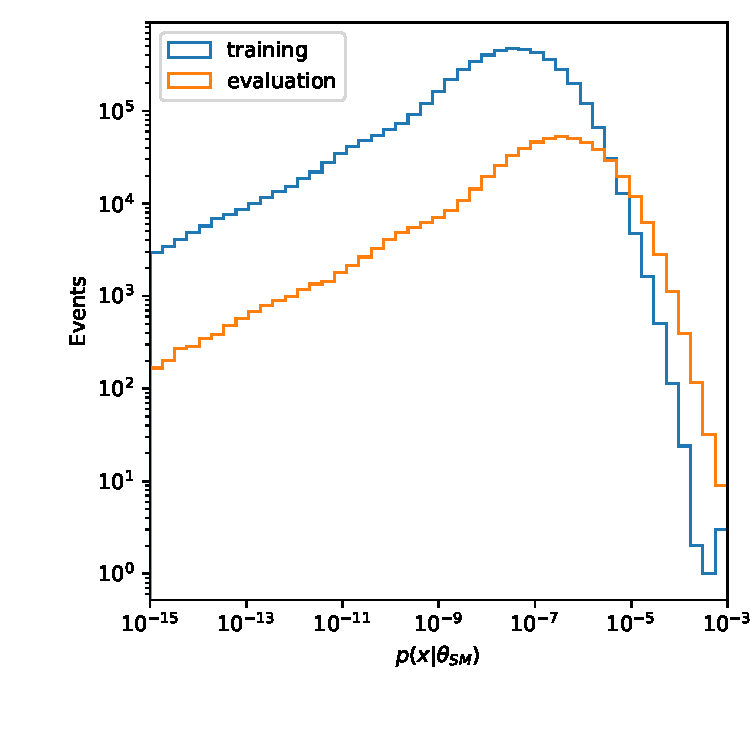
\includegraphics[width=0.45\textwidth]{figures/pointwise_tuning_2d/sample_weights.pdf}
%   \caption{Distribution of event weights for the SM hypothesis, for
%     the main training sample as well as for the final evaluation
%     sample}.
%   \label{fig:sample_weights}
% \end{figure}

We generate a sample of $5.55 \cdot 10^6$ weighted events, which we
randomly split into a main sample of $5.00 \cdot 10^6$ events for
training and intermediate testing plus a smaller sample of
$0.55 \cdot 10^6$ events for the final evaluation.

In \autoref{fig:sample_weights} we show the distribution of the event
weights in these two samples. The weights are not distributed evenly,
with individual events in the training sample carrying an individual
probability to be drawn of up to $10^{-3}$. This is, of course, far
from ideal ideal, but unfortunately a consequence of using
$\toolfont{MadMax}$.



%%%%%%%%%%%%%%%%%%%%%%%%%%%%%%%%%%%%%%%%%%%%%%%%%%%%%%%%%%%%
\subsection{Observables}
\label{sec:features}
%%%%%%%%%%%%%%%%%%%%%%%%%%%%%%%%%%%%%%%%%%%%%%%%%%%%%%%%%%%%

We train classifiers and estimate the likelihood ratio $r(\boldx)$
based on different sets of kinematic features.
%
\begin{enumerate}
\item First, we consider a simple \emph{two-dimensional feature space}
  consisting of
  % 
  \begin{itemize}
  \item the transverse momentum of the hardest jet, $p_{T,j1}$, as well as
  \item the azimuthal angle between the two jets, $\Delta \phi_{jj}$.
  \end{itemize}
  % 
  These observables are known to be sensitive to the operators of
  interest. Broadly speaking, the jet $p_T$ distribution provides a
  probe of $\ope{W}$, while $\Delta \phi_{jj}$ is more sensitive to
  $\ope{WW}$~\cite{johann_thesis, Brehmer:2016nyr}.
%
\item We extend this to a \emph{medium set}, consisting of
  %
  \begin{itemize}
    \item the energy, transverse momentum, pseudorapidity $\eta$, and azimuthal angle
  $\phi$ of each of the two jets, ordered by $p_T$;
  \item the energy, transverse momentum, pseudorapidity $\eta$, and
    azimuthal angle $\phi$ of the four-lepton system (which reconstructs the Higgs);
  \item the invariant mass of the dijet system, $m_{jj}$;
  \item the separation in pseudorapidity between the two jets,
    $\Delta \eta_{jj}$; and
  \item the separation in azimuthal angle between the two jets,
    $\Delta \phi_{jj}$.
  \end{itemize}
  %
  This set of 15 observables completely characterises the production
  of an on-shell Higgs in weak boson fusion at leading order (which
  has a five-dimensional phase space). We aim to answer the question
  whether training \toolfont{carl} on these 15 observables is enough
  to estimate the true likelihood ratio based on the fully
  differential kinematics.
%
\item In a next step, we use the \emph{full kinematics} of the
  leading-order process including the Higgs decay. We parameterise the
  four-momenta of the four leptons and the two jets with their energy,
  transverse momentum, pseudorapidity $\eta$, and azimuthal angle
  $\phi$. In this way we include 24 variables, 9 more than the 15
  dimensions of the phase space at leading
  order.\footnote{$ (2+6) \cdot 4_{\text{four-momenta}} -
    4_{\text{$E$, $p$ conservation}} - 8_{\text{on-shell conditions}}
    - 4_{\text{beam directions}} - 1_{\text{overall $\phi$}} = 15$}
%
\item Finally, we add some \emph{derived variables} to this full set
  and check whether this improves the classifier performance. In
  addition to the 24 variables of the previous set, we include the
  following quantities:
  % 
  \begin{itemize}
  \item the invariant mass of the dijet system, $m_{jj}$;
  \item the separation in pseudorapidity between the two jets,
    $\Delta \eta_{jj}$;
  \item the separation in azimuthal angle between the two jets,
    $\Delta \phi_{jj}$;
  \item the invariant masses of the two reconstructed $Z$ bosons,
    $m_{Z1}$ and $m_{Z2}$;
  \item the energy, transverse momentum, pseudorapidity, and azimuthal
    angle of the four-lepton system; and finally 
  \item the energy, transverse momentum, pseudorapidity, and azimuthal
    angle of the reconstructed $Z$ bosons.
  \end{itemize}
  % 
  All in all, this makes 42 observables. We do not (yet) explicitly
  take into account the decay angles that characterize the
  $h \to 4\ell$ decay chain since they carry less information on
  $\ope{W}$ and $\ope{WW}$ than production-side
  observables~\cite{johann_thesis, Brehmer:2016nyr}.
\end{enumerate}




%%%%%%%%%%%%%%%%%%%%%%%%%%%%%%%%%%%%%%%%%%%%%%%%%%%%%%%%%%%%
\subsection{Exact likelihood ratio}
%%%%%%%%%%%%%%%%%%%%%%%%%%%%%%%%%%%%%%%%%%%%%%%%%%%%%%%%%%%%

These samples $\{ \boldx, p (\boldx | \boldtheta ) \}$ allow for a
straightforward calculation of the truth-level likelihood ratio. When
the full set of kinematic variables is taken into account, it is given
by
%
\begin{equation}
  r_{\text{full}}(\boldx) = \frac {p(\boldx | \boldtheta_0)} {p(\boldx | \boldtheta_1)} \,.
\end{equation}
%
We compare the medium set of observables, the full kinematics, and the
full kinematics including derived observables to this exact ratio.

For the reduced two-dimensional feature space discussed in the
appendix, we first have to integrate (sum) over the unobserved
directions in phase space:
%
\begin{equation}
  r_{\text{2d}}(\boldv_0) =
  \dfrac
  {\sum\limits_{\boldx | \boldv(\boldx) \approx \boldv_0} p(\boldx | \boldtheta_0)}
  {\sum\limits_{\boldx' | \boldv(\boldx) \approx \boldv_0} p(\boldx' | \boldtheta_1)} \,.
\end{equation}
%
Here $\boldv \in \mathbf{R}^2$ are the two-dimensional observables,
$\boldx$ denote 15-dimensional phase-space vectors, and
$\boldv(\boldx) \approx \boldv_0$ means that the two-dimensional
observables calculated from $\boldx$ are (approximately) equal to
$\boldv_0$. This is realised by binning the two-dimensional feature
space and summing over all events $\boldx$ in the same bin. We use 20
equidistant bins for $\Delta \phi_{jj}$ times 25 bins for
$p_{T,j1}$. The jet momentum bins have a varying size: 10~\gev up to a
$p_T$ of 100~\gev, 20~\gev up to 200~\gev, 40~\gev up to 400~\gev,
80~\gev up to 1200~\gev, and an overflow bin for $p_T > 1200~\gev$. Note
that for simplicity we will later use $\boldx$ to label the two
observables of this process. 






%%%%%%%%%%%%%%%%%%%%%%%%%%%%%%%%%%%%%%%%%%%%%%%%%%%%%%%%%%%%
\clearpage
\section{Inference strategies}
\label{sec:strategies}
%%%%%%%%%%%%%%%%%%%%%%%%%%%%%%%%%%%%%%%%%%%%%%%%%%%%%%%%%%%%




%%%%%%%%%%%%%%%%%%%%%%%%%%%%%%%%%%%%%%%%%%%%%%%%%%%%%%%%%%%%
\subsection{Algorithms}
%%%%%%%%%%%%%%%%%%%%%%%%%%%%%%%%%%%%%%%%%%%%%%%%%%%%%%%%%%%%

A first class of algorithms approaches the inference problem point by
point in parameter space, learning the likelihood ratio
$r (\boldx; \boldtheta_0, \boldtheta_1) \equiv p(\boldx |
\boldtheta_0) / p(\boldx | \boldtheta_1)$
between a fixed pair of hypotheses. Only in the end the different
analysed pairs $(\boldtheta_0, \boldtheta_1)$ are compared and
interpolated.

Instead of estimating the likelihood ratio separately for different
pairs $(\boldtheta_0, \boldtheta_1)$, we can also train one
parameterized classifier or regressor
$\hat{r}(\boldx; \boldtheta_0 , \boldtheta_1)$. This allows us to go
beyond the likelihood-free setting and include the information from
the score when it is available, or to use physics knowledge about the
$\boldtheta$ dependence.

\dots

We consider five different inference setups. For the
\emph{likelihood-free setting}, we use the normal \toolfont{carl}
approach. We first define a ``raw'' version: for the mapping
$\hat{r} (\hat{s})$ we simply assume a perfectly trained classifier,
$\hat{s}(\boldx) = p(\boldx|\boldtheta_0) / ( p(\boldx|\boldtheta_0) +
p(\boldx|\boldtheta_1) )$.  Second, we use a calibrated version, where
we generate a new calibration histogram for each of the 1016 values of
$\boldtheta_0$ used in the evaluation. For the calibration we always
use the same (weighted) events, which is not possible in the most
general likelihood-free setup (but may be in situations like the EFT
described here).

For the setup in which the \emph{score is tractable}, we define two
parameterized estimators: one is just trained by regressing on the
score data. The second uses a combination of \toolfont{carl}'s
cross-entropy loss and the mean squared error of the score regression
problem. A parameter $\alpha$ weights these two terms in the loss
function, aiming for an approximately equal size of the two
terms. Again, we consider a raw and a calibrated version of this
setup.

Finally, we define two regressors for the case in which the
\emph{likelihood is tractable}: standard regression on $\log r$, both
for the point-by-point and the parameterized setup. For the
parameterized setup, we also use a combination of regression on
$\log r$ and on the score. The regression models are not calibrated.




%%%%%%%%%%%%%%%%%%%%%%%%%%%%%%%%%%%%%%%%%%%%%%%%%%%%%%%%%%%%
\subsection{Training samples}
%%%%%%%%%%%%%%%%%%%%%%%%%%%%%%%%%%%%%%%%%%%%%%%%%%%%%%%%%%%%

We consider four different training samples. In the \emph{baseline} setup, the
training sample consists of 1000 pairs $(\boldtheta_0, \boldtheta_1)$.
%
\begin{equation}
  \boldtheta_1 = (0.393, 0.492)
  \label{eq:theta1}
\end{equation}
%
is fixed, while the values of $\boldtheta_0$ are chosen randomly (with
a flat distribution over $[-1,1]^2]$). For each of these pairs, we
draw 5\,000 events according to $\boldtheta_0$ and 5\,000 events
according to $\boldtheta_1$. This amounts to a total of $10^7$ events.

In our alternative ``\emph{random $\boldtheta$}'' training sample draw
independent values of $\boldtheta_0$ for each event, from a flat prior
in $[-1,1]^2$. $\boldtheta_1$ is fixed as before. The sample consists
of 9998227 events, 4998047 of which were drawn according to
$\boldtheta_1$.

Finally, for some scenarios we analyse a training sample where only
the 15 basis points of the morphing procedure are used as values of
$\boldtheta_0$. Again a total of $10^7$ events are used.

In all cases, our evaluation sample consists of $100\,000$ events
drawn according to the SM. We calculate the exact likelihood ratio for
these events for a total of 1016 values of $\boldtheta_0$, 1000 of
which are the same as those used in the first training sample. Again
we fix $\boldtheta_1$ as in Equation~\eqref{eq:theta1}.



%%%%%%%%%%%%%%%%%%%%%%%%%%%%%%%%%%%%%%%%%%%%%%%%%%%%%%%%%%%%
\subsubsection{Estimator design}
%%%%%%%%%%%%%%%%%%%%%%%%%%%%%%%%%%%%%%%%%%%%%%%%%%%%%%%%%%%%

In the \emph{baseline} model, our estimators consist of a fully
connected neural network. In this way, the network can learn
(almost) any dependence on $\boldtheta$ it wants.

In addition we consider a ``\emph{physics-aware model}'' that uses the
knowledge about the compositional structure of the likelihood function
(as in the morphing setup):
%
\begin{equation}
  \hat{r} (\boldx; \boldtheta) = \sum_i w_i(\boldtheta) \, \hat{r}_i (\boldx)
\end{equation}
%
where we have explicitly left out the dependence on $\boldtheta_1$,
which we always keep fixed. The sum goes over the 15 basis samples
used in the morphing setup, and the functions $w_i(\boldtheta)$ are
analytically known. Following this structure, our network consists of
15 independent estimators $\hat{r}_i (\boldx)$, weighted with the
$w_i(\boldtheta)$.

For all architectures, We use between one and three hidden layers of
100 units with $\tanh$ activation functions for the baseline model,
and two hidden layers of 50 units with $\tanh$ activation functions.
We implement all setups in \toolfont{keras} with a
\toolfont{TensorFlow} backend inside a \toolfont{sklearn} wrapper and
train for 20 epochs with early stopping. 



%%%%%%%%%%%%%%%%%%%%%%%%%%%%%%%%%%%%%%%%%%%%%%%%%%%%%%%%%%%%
\subsubsection{Metrics}
\label{sec:metrics}
%%%%%%%%%%%%%%%%%%%%%%%%%%%%%%%%%%%%%%%%%%%%%%%%%%%%%%%%%%%%

\dots



%%%%%%%%%%%%%%%%%%%%%%%%%%%%%%%%%%%%%%%%%%%%%%%%%%%%%%%%%%%%
\subsubsection{Uncertainty diagnostics}
\label{sec:diagnostics}
%%%%%%%%%%%%%%%%%%%%%%%%%%%%%%%%%%%%%%%%%%%%%%%%%%%%%%%%%%%%

We are experimenting with diagnostic tools that might provide some
measure of the uncertainty of the estimators $\hat{r}(\boldx)$. There are different ideas:
%
\begin{enumerate}
\item \emph{Ensemble variance}: repeating the full calculation with
  different random seeds, one can extract an uncertainty measure from
  the ensemble variance. This would only capture statistical
  uncertainties, not a systematic bias. Obviously this increases the
  computational cost.
  % 
\item \emph{Denominator variation}: the relative log likelihood
  contours (compared to the best-fit point) should not depend on the
  choice of the denominator hypothesis
  $\boldtheta_1$~\cite{Cranmer:2015bka}. We can therefore use
  quantities like
  % 
  \begin{multline}
    \Delta \log \hat{r} (\boldx; \boldtheta_0, \boldtheta_1) 
    = \Bigl| (\log \hat{r} (\boldx; \boldtheta_0, \boldtheta_1) - \max_\boldtheta \log \hat{r} (\boldx; \boldtheta, \boldtheta_1) ) \\
      - (\log \hat{r}' (\boldx; \boldtheta_0, \boldtheta_1') - \max_\boldtheta \log \hat{r}' (\boldx; \boldtheta_0, \boldtheta_1') ) \Bigr| \,.
    \label{eq:diagnostics3}
  \end{multline}
  % 
  as a measure of systematic uncertainties. Probably such a number
  only presents a lower bound for the true uncertainty. Again, this
  increases the computational cost.
  % 
\item \emph{Toy experiments}: we perform a series of mock experiments
  with different numbers of events and calculate the variance in the
  distribution of $\log \hat{r}{\boldx}$ as a function of the number
  of events. We fit the variance as a function of the event number
  with
  % 
  \begin{equation}
    \var [\log \hat{r}(\boldx; \boldtheta_0, \boldtheta_1) ] (n) = a/n + b \,.
  \end{equation}
  % 
  Then $\sqrt{a/n}$ represents the statistical uncertainty from a
  limited number of events, while
  % 
  \begin{equation}
    \Delta \log \hat{r} (\boldx; \boldtheta_0, \boldtheta_1) = \sqrt{b}
    \label{eq:diagnostics1}
  \end{equation}
  % 
  might provide a measure of a residual systematic uncertainty in the
  expectation values with large $n$. There is no guarantee that this
  strategy works.
  % 
\item \emph{Identity check}: for $\boldtheta_0 = \boldtheta_1$ the log
  likelihood ratio should identically vanish. A non-zero value of
  % 
  \begin{equation}
    \Delta \log \hat{r} (\boldx) = \log \hat{r}(\boldx; \boldtheta_0 = \boldtheta_1, \boldtheta_1) 
    \label{eq:diagnostics2}
  \end{equation}
  % 
  might therefore hint at a systematic uncertainty. Again, there is no
  guarantee that this number says anything about the behaviour at other
  values of $\boldtheta_0$. Also, any constant bias in
  $ \log \hat{r} (\boldx) $ would cancel out in the likelihood contours,
  which consider the difference in the log likelihood with respect to
  the best-fit point.
%
\item \emph{Score expectation value}: we know that
  $E[\mathbf{t}(\boldx | \boldtheta_0) | \boldtheta_0] = 0$. Perhaps
  there is a way to translate non-zero expectation values to an
  uncertainty measure on $\log r(\boldx)$?
\end{enumerate}





%%%%%%%%%%%%%%%%%%%%%%%%%%%%%%%%%%%%%%%%%%%%%%%%%%%%%%%%%%%%
\clearpage
\section{Results}
%%%%%%%%%%%%%%%%%%%%%%%%%%%%%%%%%%%%%%%%%%%%%%%%%%%%%%%%%%%%




%%%%%%%%%%%%%%%%%%%%%%%%%%%%%%%%%%%%%%%%%%%%%%%%%%%%%%%%%%%%
\subsection{Overview}
%%%%%%%%%%%%%%%%%%%%%%%%%%%%%%%%%%%%%%%%%%%%%%%%%%%%%%%%%%%%

Tables~\ref{tbl:comparison1} to
\ref{tbl:comparison_score} compare the performance of all
different setups tested.

\begin{table}
  \small
  \begin{tabular}{ll rr rr}
    \toprule
    Algorithm & Setup & \multicolumn{2}{c}{$\MSE_\boldx \left[ \log  r(\boldx; \boldtheta_0, \boldtheta_1) \right]$}
    & \multicolumn{2}{c}{$\MSE_\boldtheta \left[ E[\log r(\boldx;
      \boldtheta, \boldtheta_{\text{den}})] \right]$} \\
    \cmidrule{3-4} \cmidrule{5-6}
    && $\boldtheta_0 = \boldtheta_{T}$ & $\boldtheta_0 = \boldtheta_{NT}$
      & $\boldtheta_{\text{den}} = \boldtheta_1$ & $\boldtheta_{\text{den}} = \hat{\boldtheta}_{\text{MLE}}$ \\
    \midrule
   PbP carl (raw) & PbP (1) & $0.206$ & $0.229$ & $50.54$ & $5.98$\\
    & PbP (2) & $0.177$ & $0.203$ & $48.99$ & $4.75$\\
    & PbP (3) & $0.201$ & $0.272$ & $49.31$ & $5.97$\\
    & PbP learning $\log r(\boldx)$ (1) & $0.189$ & $0.193$ & $49.15$ & $\mathbf{4.14}$\\
    & PbP learning $\log r(\boldx)$ (2) & $0.269$ & $0.196$ & $48.51$ & $4.59$\\
    & PbP learning $\log r(\boldx)$ (3) & $\mathbf{0.114}$ & $\mathbf{0.157}$ & $\mathbf{47.81}$ & $4.80$\\
   \midrule
   PbP carl (cal.) & PbP (1) & $0.094$ & $0.121$ & $3.91$ & $\mathbf{3.82}$\\
    & PbP (2) & $0.139$ & $0.239$ & $3.91$ & $3.87$\\
    & PbP (3) & $0.099$ & $0.132$ & $3.95$ & $3.90$\\
    & PbP learning $\log r(\boldx)$ (1) & $0.097$ & $0.194$ & $3.93$ & $3.91$\\
    & PbP learning $\log r(\boldx)$ (2) & $\mathbf{0.087}$ & $0.155$ & $\mathbf{3.88}$ & $3.85$\\
    & PbP learning $\log r(\boldx)$ (3) & $0.113$ & $\mathbf{0.100}$ & $3.95$ & $4.36$\\
   \midrule
   Param carl (raw) & Baseline (1) & $0.040$ & $0.074$ & $2.78$ & $0.72$\\
    & Baseline (2) & $0.083$ & $0.116$ & $29.68$ & $5.49$\\
    & Baseline (3) & $0.037$ & $\mathbf{0.051}$ & $4.80$ & $2.64$\\
    & Random $\boldtheta$ (1) & $0.047$ & $0.066$ & $1.41$ & $1.53$\\
    & Random $\boldtheta$ (2) & $\mathbf{0.037}$ & $0.054$ & $0.85$ & $0.70$\\
    & Random $\boldtheta$ (3) & $0.040$ & $0.055$ & $\mathbf{0.26}$ & $\mathbf{0.20}$\\
    & Physics-aware (1) &  &  &  & \\
    & Physics-aware (2) &  &  &  & \\
    & Physics-aware (3) &  &  &  & \\
   \midrule
   Param carl (cal.) & Baseline (1) & $0.033$ & $0.050$ & $0.24$ & $0.41$\\
    & Baseline (2) & $\mathbf{0.027}$ & $\mathbf{0.038}$ & $0.10$ & $0.09$\\
    & Baseline (3) & $0.047$ & $0.062$ & $0.58$ & $0.61$\\
    & Random $\boldtheta$ (1) & $0.034$ & $0.048$ & $0.09$ & $0.30$\\
    & Random $\boldtheta$ (2) & $0.041$ & $0.055$ & $\mathbf{0.03}$ & $\mathbf{0.04}$\\
    & Random $\boldtheta$ (3) & $0.046$ & $0.064$ & $0.64$ & $0.50$\\
    & Physics-aware (1) &  &  &  & \\
    & Physics-aware (2) &  &  &  & \\
    & Physics-aware (3) &  &  &  & \\
    \bottomrule
  \end{tabular}
  \caption{Comparison of different inference strategies, part 1.
    In this table we show likelihood-free strategies based on a
    point-by-point (PbP) or parameterized setup.
    The numbers in brackets denote the number of hidden layers in the
    neural networks.  We show two types metrics: the mean squared
    error of $\log r$ for a fixed pair of hypotheses
    over different phase-space points and the mean squared error of the expectation 
    value of $\log r$ for different pairs of hypotheses. For the first case,
    the benchmark point $\boldtheta_{T}$ was part of all training samples
    (except for the random $\boldtheta$ sample), while the benchmark point
    $\boldtheta_{NT}$ is unknown to the parameterized models (it was still part
    of the point-by-point training). In the latter
    case, the expectation value sums over $\boldx$ following the SM
    distribution.}
  \label{tbl:comparison1}
\end{table}


\begin{table}
  \small
  \begin{tabular}{ll rr rr}
    \toprule
    Algorithm & Setup & \multicolumn{2}{c}{$\MSE_\boldx \left[ \log  r(\boldx; \boldtheta_0, \boldtheta_1) \right]$}
    & \multicolumn{2}{c}{$\MSE_\boldtheta \left[ E[\log r(\boldx; \boldtheta, \boldtheta_{\text{den}})] \right]$} \\
    \cmidrule{3-4} \cmidrule{5-6}
    && $\boldtheta_0 = \boldtheta_{T}$ & $\boldtheta_0 = \boldtheta_{NT}$
      & $\boldtheta_{\text{den}} = \boldtheta_1$ & $\boldtheta_{\text{den}} = \hat{\boldtheta}_{\text{MLE}}$ \\
   \midrule
   Param score (raw) & Baseline (1) & $\mathbf{0.060}$ & $0.067$ & $0.23$ & $0.25$\\
    & Baseline (2) & $0.060$ & $\mathbf{0.064}$ & $\mathbf{0.16}$ & $\mathbf{0.06}$\\
    & Baseline (3) & $0.104$ & $0.110$ & $15.30$ & $0.09$\\
    & Random $\boldtheta$ (1) & $0.099$ & $0.135$ & $3.51$ & $3.57$\\
    & Random $\boldtheta$ (2) & $0.082$ & $0.113$ & $3.76$ & $3.19$\\
    & Random $\boldtheta$ (3) & $0.135$ & $0.177$ & $14.09$ & $3.20$\\
    & Physics-aware (1) &  &  &  & \\
    & Physics-aware (2) &  &  &  & \\
    & Physics-aware (3) &  &  &  & \\
   \midrule
   Param score (cal.) & Baseline (1) & $0.100$ & $0.105$ & $0.96$ & $0.90$\\
    & Baseline (2) & $\mathbf{0.076}$ & $\mathbf{0.094}$ & $\mathbf{0.43}$ & $\mathbf{0.43}$\\
    & Baseline (3) &  &  &  & \\
    & Random $\boldtheta$ (1) & $0.088$ & $0.172$ & $2.01$ & $2.15$\\
    & Random $\boldtheta$ (2) & $0.115$ & $0.533$ & $2.36$ & $2.36$\\
    & Random $\boldtheta$ (3) &  &  &  & \\
    & Physics-aware (1) &  &  &  & \\
    & Physics-aware (2) &  &  &  & \\
    & Physics-aware (3) &  &  &  & \\
   \midrule
   Param carl + score (raw) & Baseline (1) & $0.037$ & $0.049$ & $2.11$ & $0.19$\\
    & Baseline (2) & $\mathbf{0.014}$ & $\mathbf{0.016}$ & $\mathbf{0.66}$ & $0.16$\\
    & Baseline (3) & $0.041$ & $0.047$ & $10.99$ & $\mathbf{0.15}$\\
    & Random $\boldtheta$ (1) & $0.050$ & $0.082$ & $1.53$ & $3.62$\\
    & Random $\boldtheta$ (2) & $0.038$ & $0.063$ & $2.08$ & $3.50$\\
    & Random $\boldtheta$ (3) & $0.053$ & $0.074$ & $3.01$ & $4.20$\\
    & Physics-aware (1) &  &  &  & \\
    & Physics-aware (2) &  &  &  & \\
    & Physics-aware (3) &  &  &  & \\
   \midrule
   Param carl + score (cal.) & Baseline (1) & $0.028$ & $0.041$ & $0.07$ & $\mathbf{0.07}$\\
    & Baseline (2) & $\mathbf{0.012}$ & $\mathbf{0.014}$ & $\mathbf{0.04}$ & $0.09$\\
    & Baseline (3) & $0.028$ & $0.023$ & $0.56$ & $0.46$\\
    & Random $\boldtheta$ (1) & $0.037$ & $0.058$ & $0.49$ & $0.97$\\
    & Random $\boldtheta$ (2) & $0.024$ & $0.035$ & $0.32$ & $0.47$\\
    & Random $\boldtheta$ (3) & $0.034$ & $0.047$ & $0.63$ & $0.98$\\
    & Physics-aware (1) &  &  &  & \\
    & Physics-aware (2) &  &  &  & \\
    & Physics-aware (3) &  &  &  & \\
    \bottomrule
  \end{tabular}
  \caption{Comparison of different inference strategies, part 2.
    In this table we show parameterized architectures that utilize the score information.
    The numbers in brackets denote the number of hidden layers in the
    neural networks.  We show two types metrics: the mean squared
    error of $\log r$ for a fixed pair of hypotheses
    over different phase-space points and the mean squared error of the expectation 
    value of $\log r$ for different pairs of hypotheses. For the first case,
    the benchmark point $\boldtheta_{T}$ was part of all training samples
    (except for the random $\boldtheta$ sample), while the benchmark point
    $\boldtheta_{NT}$ is unknown to the parameterized models (it was still part
    of the point-by-point training). In the latter
    case, the expectation value sums over $\boldx$ following the SM
    distribution.}
  \label{tbl:comparison2}
\end{table}


\begin{table}
  \small
  \begin{tabular}{ll rr rr}
    \toprule
    Algorithm & Setup & \multicolumn{2}{c}{$\MSE_\boldx \left[ \log  r(\boldx; \boldtheta_0, \boldtheta_1) \right]$}
    & \multicolumn{2}{c}{$\MSE_\boldtheta \left[ E[\log r(\boldx; \boldtheta, \boldtheta_{\text{den}})] \right]$} \\
    \cmidrule{3-4} \cmidrule{5-6}
    && $\boldtheta_0 = \boldtheta_{T}$ & $\boldtheta_0 = \boldtheta_{NT}$
      & $\boldtheta_{\text{den}} = \boldtheta_1$ & $\boldtheta_{\text{den}} = \hat{\boldtheta}_{\text{MLE}}$ \\
    \midrule
   PbP regression (raw) & PbP (1) & $0.011$ & $0.015$ & $3.79$ & $3.92$\\
    & PbP (2) & $0.005$ & $\mathbf{0.005}$ & $3.78$ & $\mathbf{3.83}$\\
    & PbP (3) & $\mathbf{0.004}$ & $0.006$ & $\mathbf{3.60}$ & $4.02$\\
   \midrule
   Param regression (raw) & Baseline (1) & $0.015$ & $0.022$ & $0.12$ & $0.12$\\
    & Baseline (2) & $\mathbf{0.004}$ & $\mathbf{0.005}$ & $0.16$ & $0.14$\\
    & Baseline (3) & $0.007$ & $0.007$ & $0.30$ & $0.29$\\
    & Random $\boldtheta$ (1) & $0.015$ & $0.021$ & $0.40$ & $0.22$\\
    & Random $\boldtheta$ (2) & $0.005$ & $0.007$ & $0.20$ & $\mathbf{0.02}$\\
    & Random $\boldtheta$ (3) & $0.007$ & $0.008$ & $\mathbf{0.04}$ & $0.03$\\
    & Physics-aware (1) &  &  &  & \\
    & Physics-aware (2) &  &  &  & \\
    & Physics-aware (3) &  &  &  & \\
   \midrule
   Param regr.\ + score (raw) & Baseline (1) &  &  &  & \\
    & Baseline (2) &  &  &  & \\
    & Baseline (3) &  &  &  & \\
    & Random $\boldtheta$ (1) &  &  &  & \\
    & Random $\boldtheta$ (2) &  &  &  & \\
    & Random $\boldtheta$ (3) &  &  &  & \\
    & Physics-aware (1) &  &  &  & \\
    & Physics-aware (2) &  &  &  & \\
    & Physics-aware (3) &  &  &  & \\
    \bottomrule
  \end{tabular}
  \caption{Comparison of different inference strategies, part 3.
    In this table we show point-by-point (PbP) and parameterized
    architectures that require a tractable likelihood.
    The numbers in brackets denote the number of hidden layers in the
    neural networks.  We show two types metrics: the mean squared
    error of $\log r$ for a fixed pair of hypotheses
    over different phase-space points and the mean squared error of the expectation 
    value of $\log r$ for different pairs of hypotheses. For the first case,
    the benchmark point $\boldtheta_{T}$ was part of all training samples
    (except for the random $\boldtheta$ sample), while the benchmark point
    $\boldtheta_{NT}$ is unknown to the parameterized models (it was still part
    of the point-by-point training). In the latter
    case, the expectation value sums over $\boldx$ following the SM
    distribution.}
  \label{tbl:comparison3}
\end{table}


\begin{table}
  \small
  \begin{tabular}{ll rr rr}
    \toprule
    Algorithm & Setup & \multicolumn{2}{c}{$\MSE_\boldx \left[ \boldt (\boldx; \boldtheta_0, \boldtheta_1) \right]$} \\
    \cmidrule{3-4} 
    && $\boldtheta_0 = \boldtheta_{T}$ & $\boldtheta_0 = \boldtheta_{NT}$ \\
    \midrule
   Param carl & Baseline (1) & $\mathbf{0.42}$ & $\mathbf{0.81}$\\
    & Baseline (2) & $1.12$ & $1.46$\\
    & Baseline (3) & $4.29$ & $2.85$\\
    & Random $\boldtheta$ (1) & $0.43$ & $0.85$\\
    & Random $\boldtheta$ (2) & $1.20$ & $1.45$\\
    & Random $\boldtheta$ (3) & $3.21$ & $3.31$\\
    & Physics-aware (1) &  & \\
    & Physics-aware (2) &  & \\
    & Physics-aware (3) &  & \\
   \midrule
   Param score & Baseline (1) & $0.19$ & $0.48$\\
    & Baseline (2) & $\mathbf{0.09}$ & $\mathbf{0.22}$\\
    & Baseline (3) & $0.10$ & $0.23$\\
    & Random $\boldtheta$ (1) & $0.40$ & $0.77$\\
    & Random $\boldtheta$ (2) & $0.37$ & $0.72$\\
    & Random $\boldtheta$ (3) & $0.40$ & $0.75$\\
    & Physics-aware (1) &  & \\
    & Physics-aware (2) &  & \\
    & Physics-aware (3) &  & \\
   \midrule
   Param carl + score & Baseline (1) & $0.24$ & $0.55$\\
    & Baseline (2) & $\mathbf{0.12}$ & $\mathbf{0.27}$\\
    & Baseline (3) & $0.15$ & $0.34$\\
    & Random $\boldtheta$ (1) & $0.38$ & $0.77$\\
    & Random $\boldtheta$ (2) & $0.36$ & $0.71$\\
    & Random $\boldtheta$ (3) & $0.37$ & $0.71$\\
    & Physics-aware (1) &  & \\
    & Physics-aware (2) &  & \\
    & Physics-aware (3) &  & \\
   \midrule
   Param regression & Baseline (1) & $0.27$ & $0.59$\\
    & Baseline (2) & $\mathbf{0.16}$ & $\mathbf{0.25}$\\
    & Baseline (3) & $0.30$ & $0.48$\\
    & Random $\boldtheta$ (1) & $0.28$ & $0.64$\\
    & Random $\boldtheta$ (2) & $0.23$ & $0.30$\\
    & Random $\boldtheta$ (3) & $0.46$ & $0.84$\\
    & Physics-aware (1) &  & \\
    & Physics-aware (2) &  & \\
    & Physics-aware (3) &  & \\
   \midrule
   Param regr.\ + score & Baseline (1) &  & \\
    & Baseline (2) &  & \\
    & Baseline (3) &  & \\
    & Random $\boldtheta$ (1) &  & \\
    & Random $\boldtheta$ (2) &  & \\
    & Random $\boldtheta$ (3) &  & \\
    & Physics-aware (1) &  & \\
    & Physics-aware (2) &  & \\
    & Physics-aware (3) &  & \\
    \bottomrule
  \end{tabular}
  \caption{Comparison of different inference strategies, part 4.
    In this table we compare the estimation of the scores in the
    different parameterized models. The benchmark point $\boldtheta_{T}$
    was part of all training samples (except for the random $\boldtheta$ sample),
    while the benchmark point $\boldtheta_{NT}$ is unknown to the parameterized
    models (it was still part of the point-by-point training).
    The numbers in brackets denote the number of hidden layers in the
    neural networks.}
  \label{tbl:comparison_score}
\end{table}


%%%%%%%%%%%%%%%%%%%%%%%%%%%%%%%%%%%%%%%%%%%%%%%%%%%%%%%%%%%%
\subsection{Baseline results}
%%%%%%%%%%%%%%%%%%%%%%%%%%%%%%%%%%%%%%%%%%%%%%%%%%%%%%%%%%%%

We show the results of the parameterized baseline experiments in
Figures~\ref{fig:baseline_r_histo} to
\ref{fig:baseline_likelihood_ratio}. We find that
calibration is important, and that the combinatino of
$\toolfont{carl}$ with score information works well. The tested
diagnostic tool for uncertainties, unfortunately, does not seem to be
particularly useful: it wrongly assisngs sizeable errors to the ground
truth.

\begin{figure}
  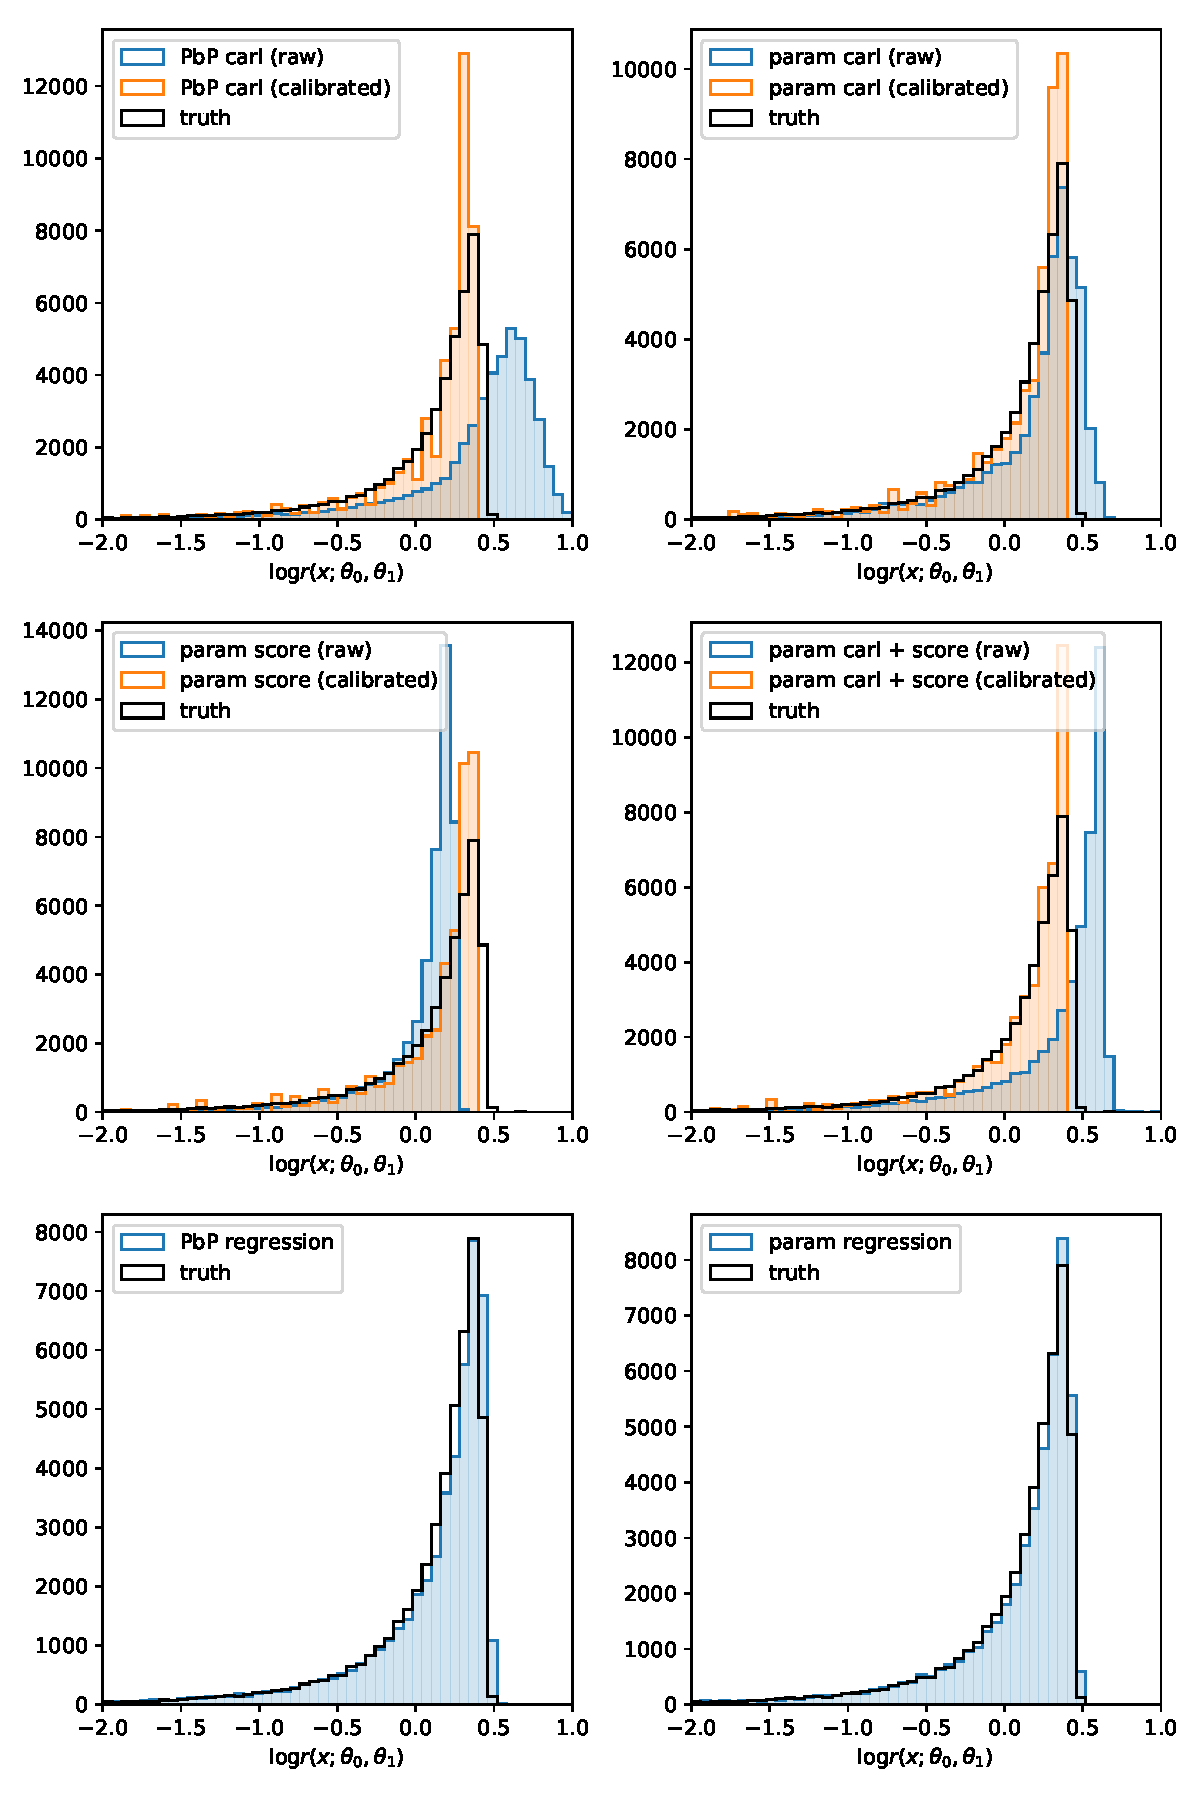
\includegraphics[width=\textwidth]{figures/results/r_histograms_vanilla.pdf}%
  \caption{Likelihood ratio histograms for individual phase-space points
    $\boldx$, for one particular hypothesis comparison
    $(\boldtheta_0, \boldtheta_1)$.  We show the baseline version of
    the different parameterized models.}
  \label{fig:baseline_r_histo}
\end{figure}

\begin{figure}
  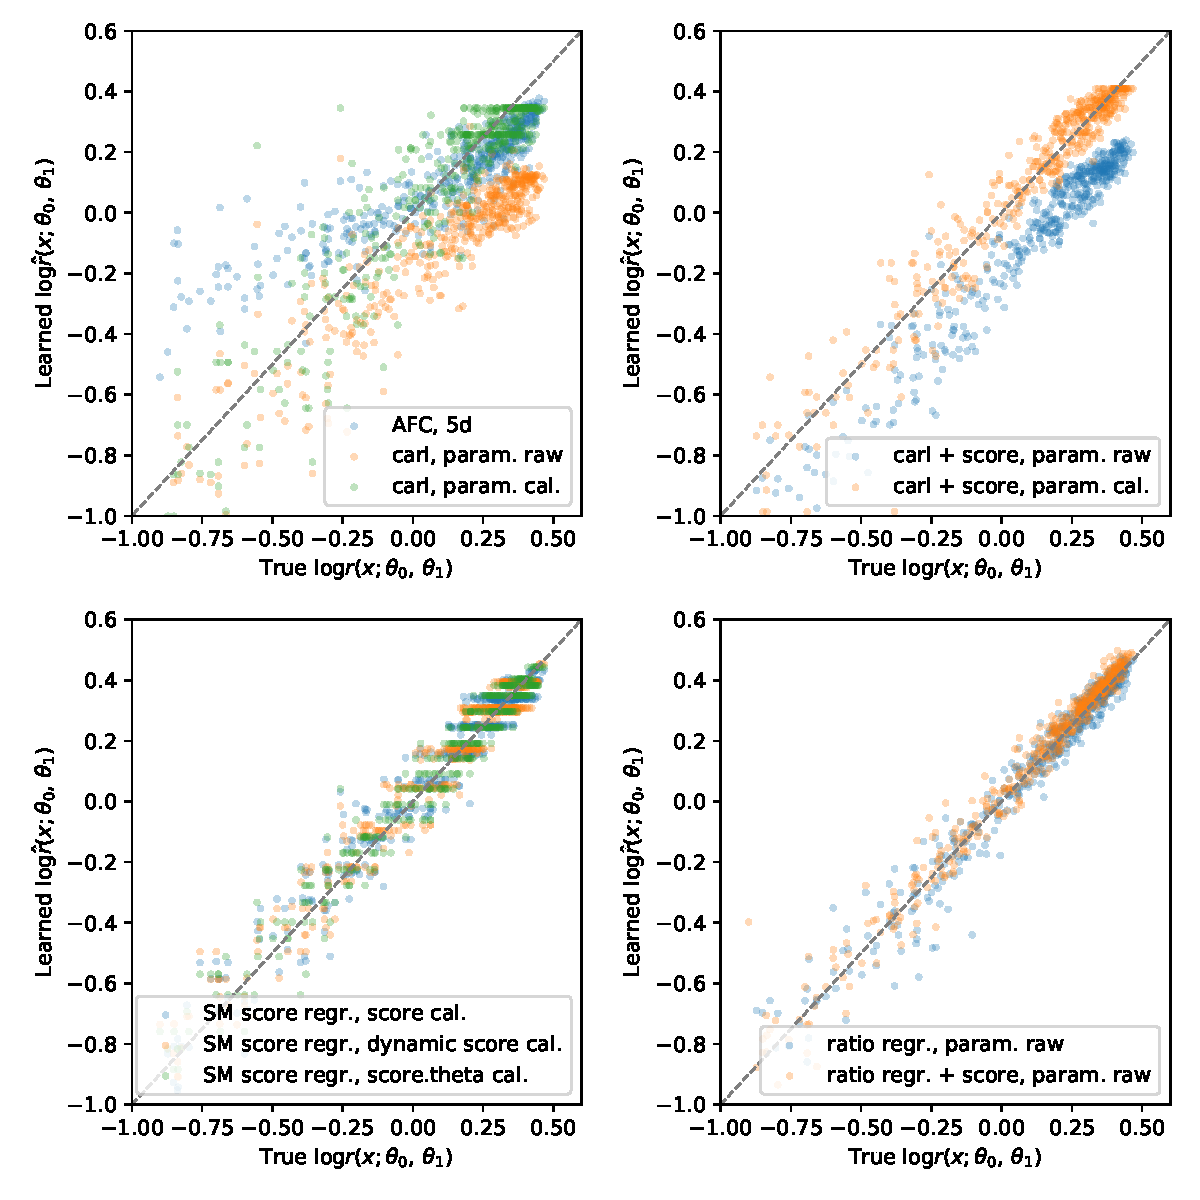
\includegraphics[width=\textwidth]{figures/results/r_scatter_vanilla.pdf}%
  \caption{Likelihood ratio scatter plot for individual phase-space points
    $\boldx$, for one particular hypothesis comparison
    $(\boldtheta_0, \boldtheta_1)$.  We show the baseline version of
    the different parameterized models.}
  \label{fig:baseline_r_scatter}
\end{figure}

\begin{figure}
  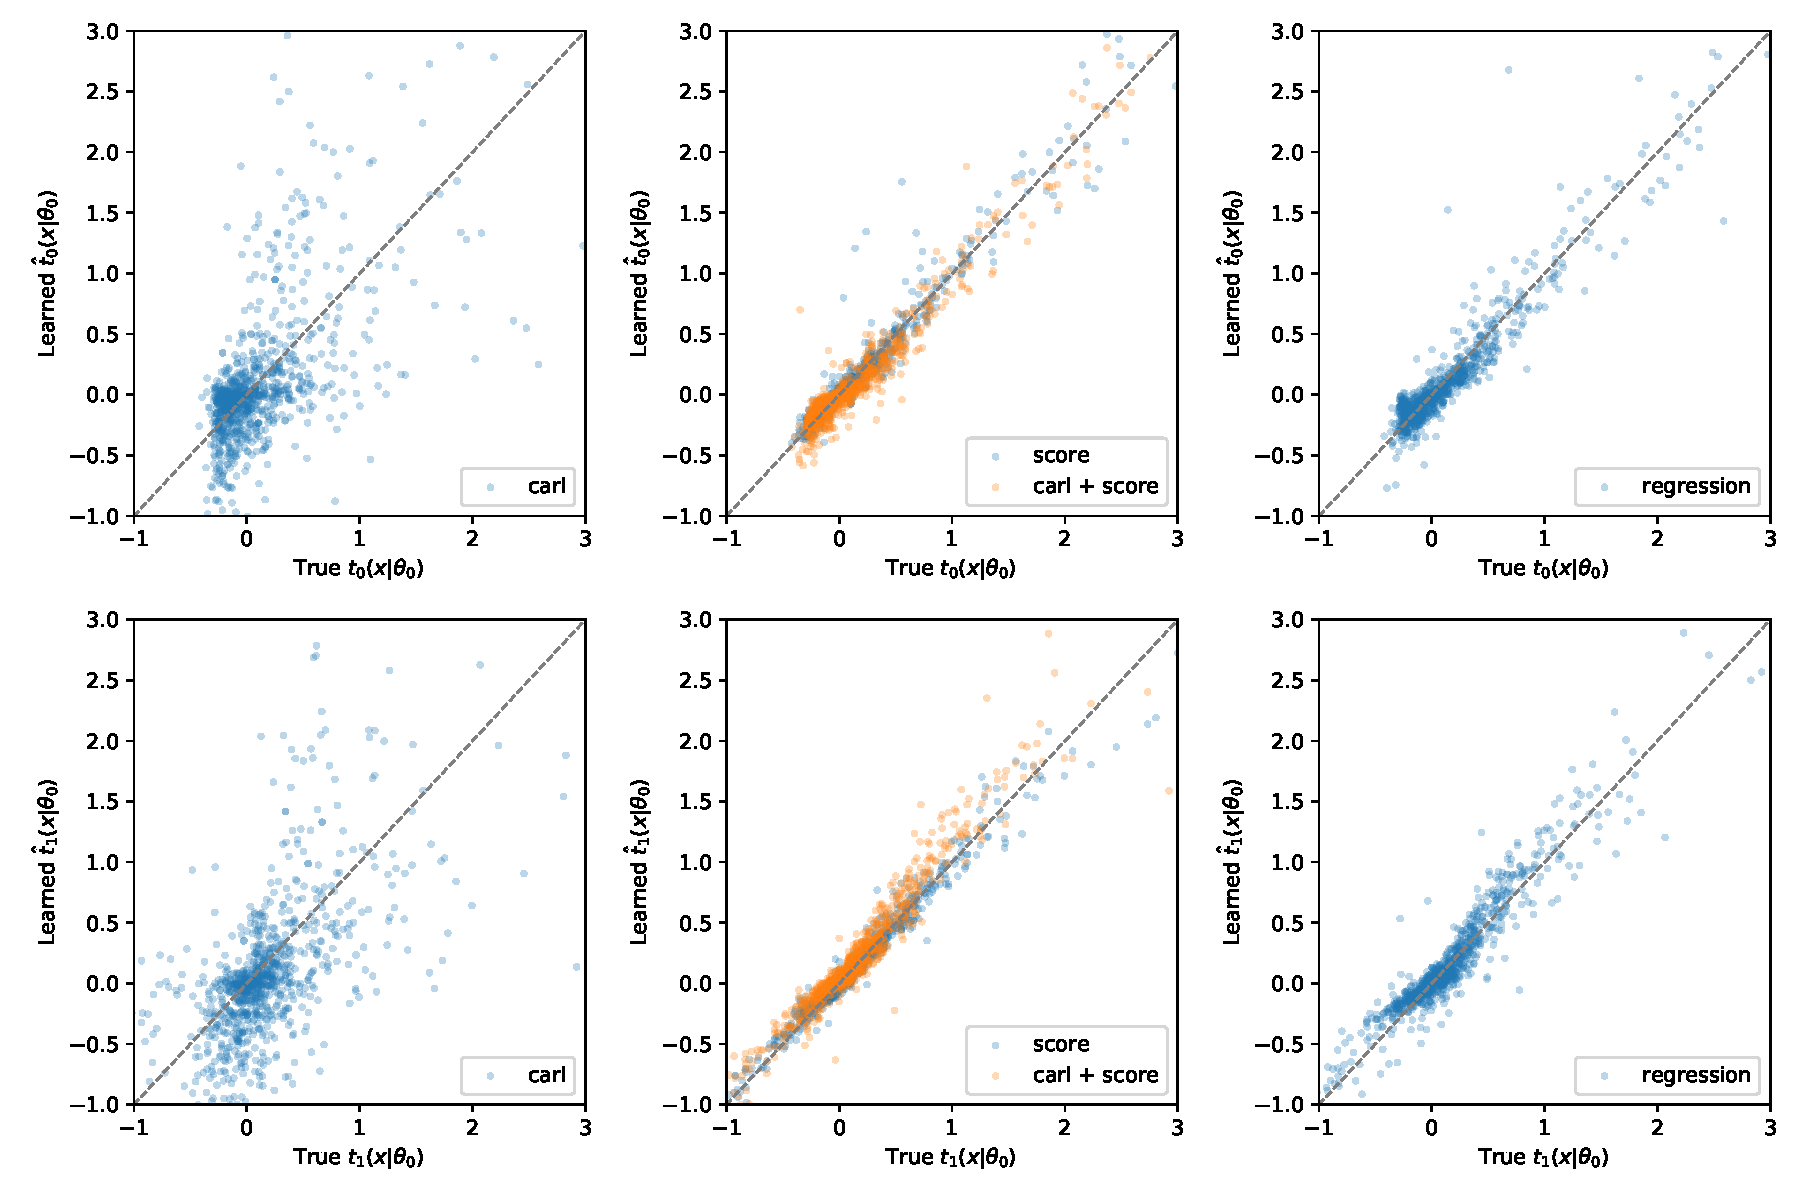
\includegraphics[width=\textwidth]{figures/results/score_scatter_vanilla.pdf}%
  \caption{Score scatter plots for individual phase-space points $\boldx$, for one
    particular hypothesis comparison $(\boldtheta_0, \boldtheta_1)$.
    We show the baseline version of the different parameterized
    models.}
  \label{fig:baseline_score_scatter}
\end{figure}

\begin{figure}
  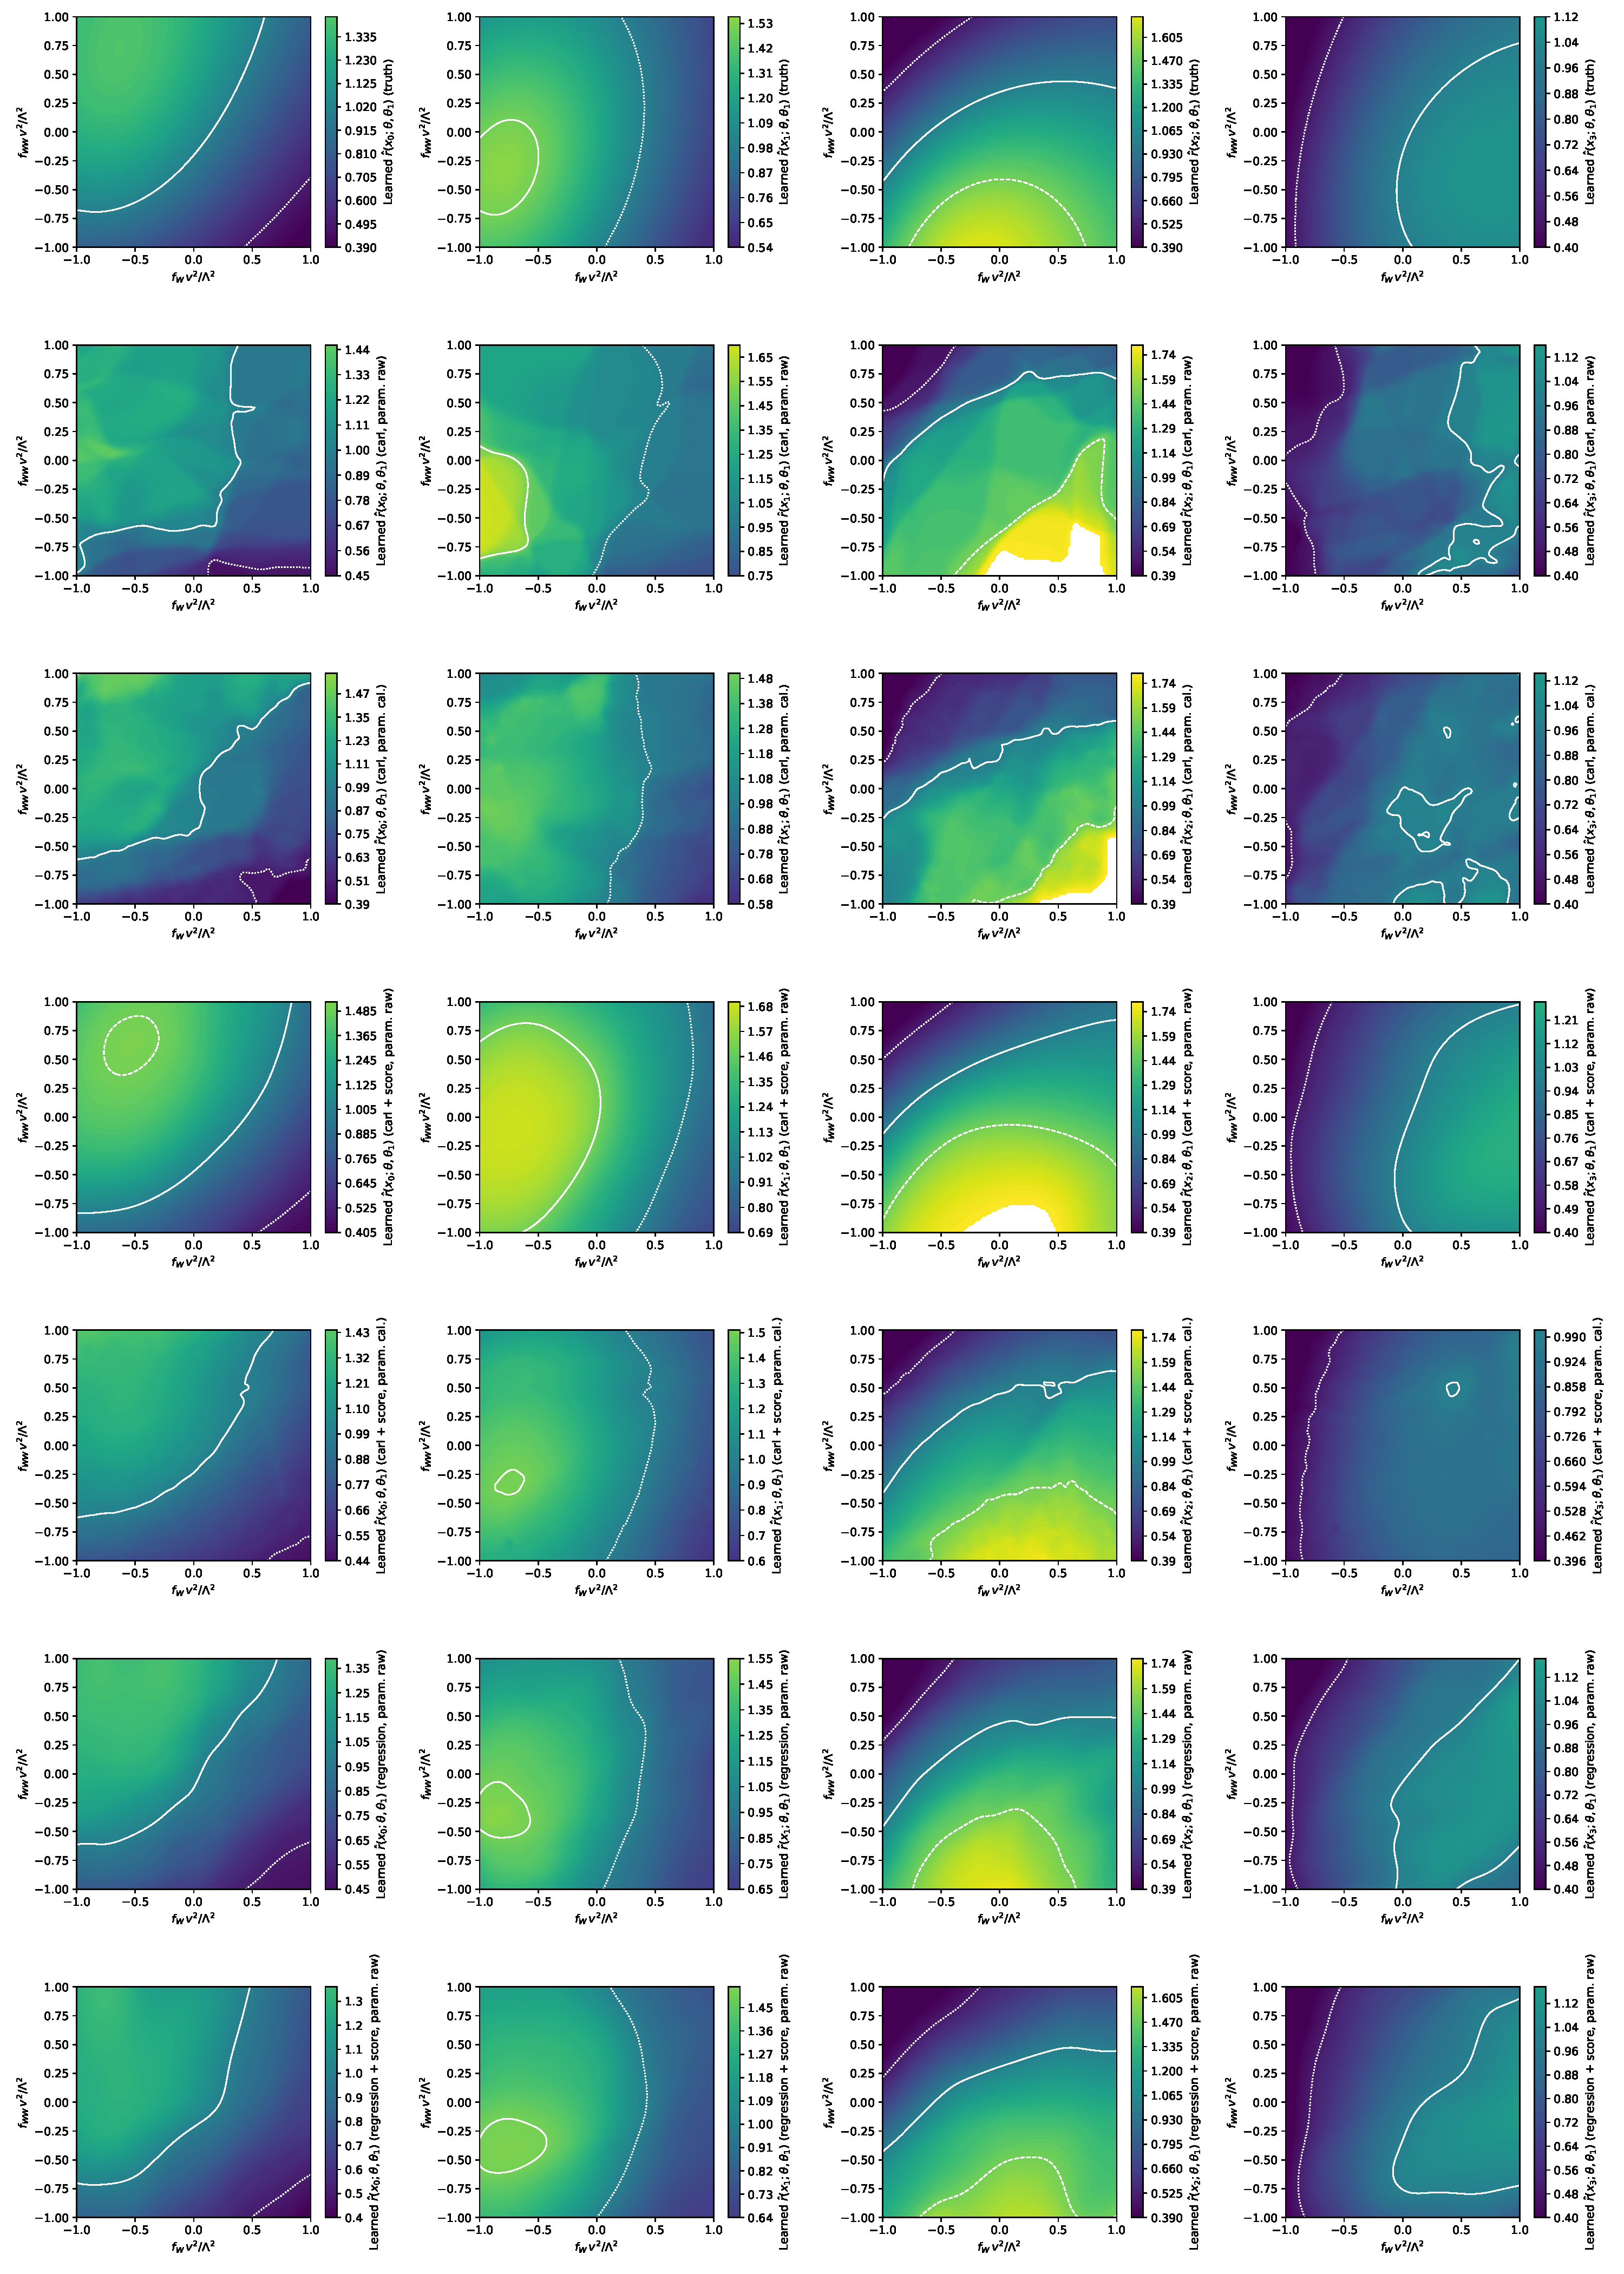
\includegraphics[width=\textwidth]{figures/results/theta_dependence_comparison_vanilla.pdf}%
  \caption{Exact and estimated likelihood ratios as a function of
    $\boldtheta_0$, for four different individual events $\boldx$
    (columns). We show the baseline version of the different
    parameterized models (rows).}
  \label{fig:baseline_theta_dependence}
\end{figure}

\begin{figure}
  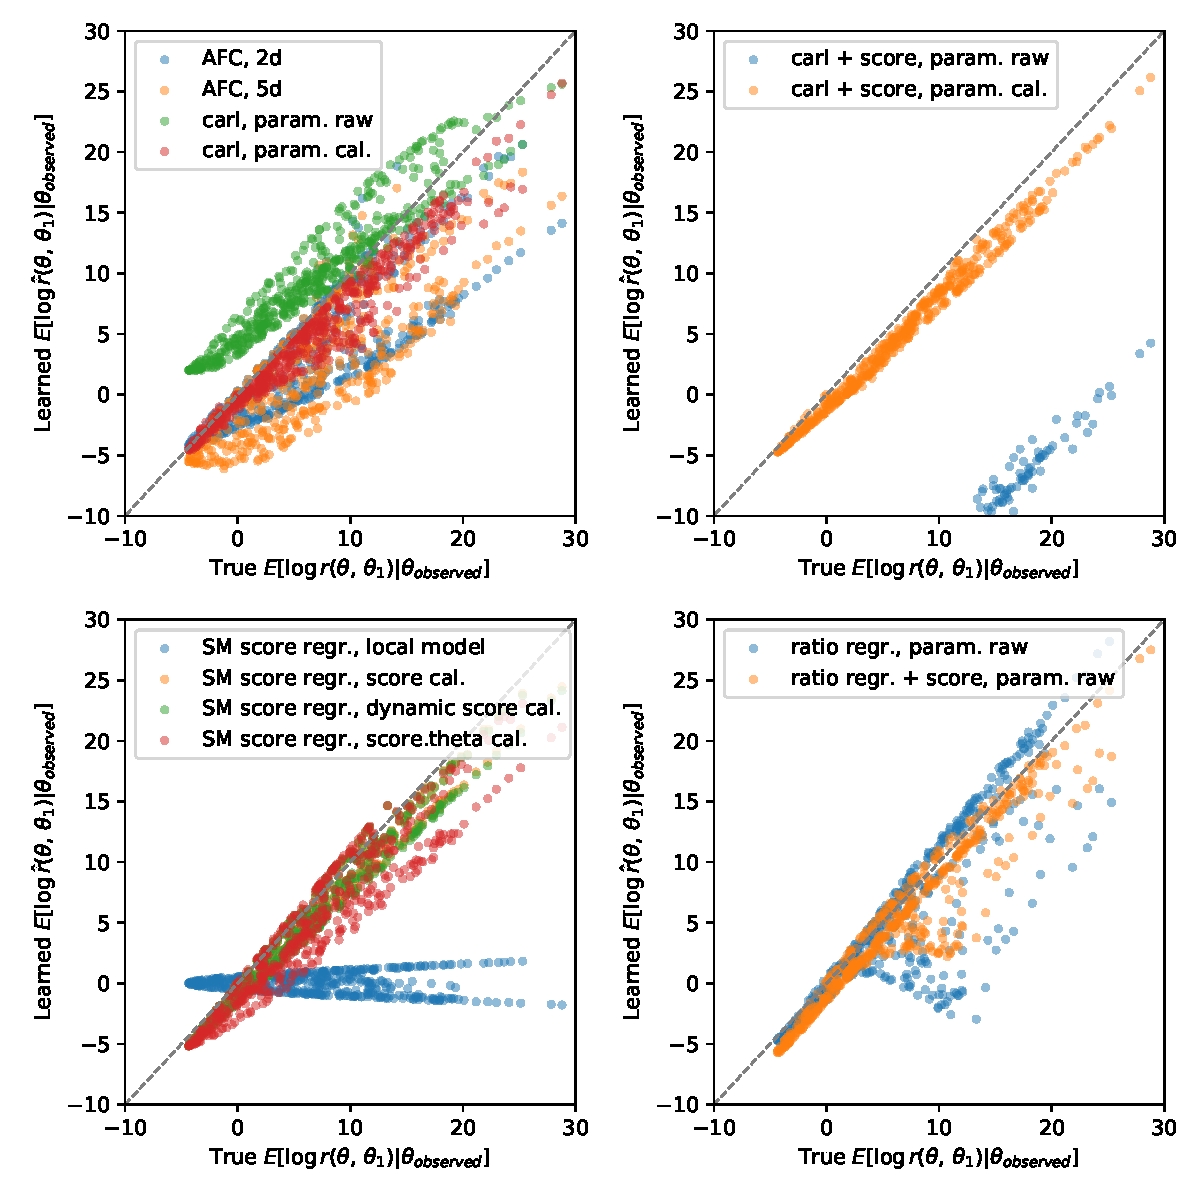
\includegraphics[width=\textwidth]{figures/results/expected_likelihood_scatter_vanilla.pdf}%
  \caption{Scatter plot of the expected likelihood ratios for
    different values of $\boldtheta_0$, taking the expectation value
    over $\boldx$. We show the baseline version of the different
    parameterized models.}
  \label{fig:baseline_likelihood_ratio}
\end{figure}

\begin{figure}
  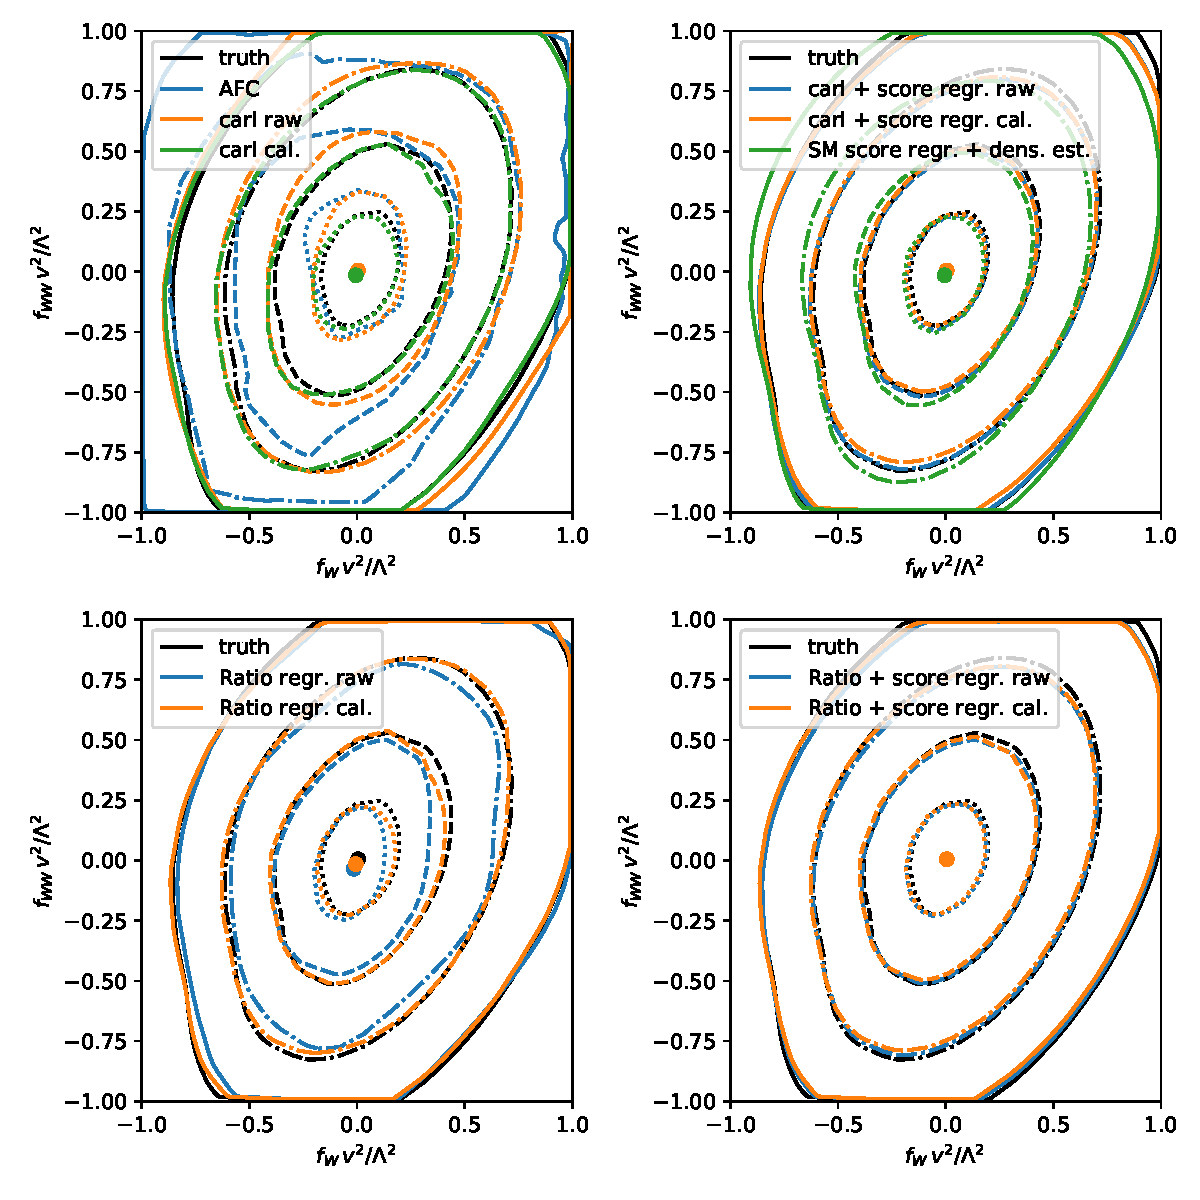
\includegraphics[width=\textwidth]{figures/results/likelihood_contours_vanilla.pdf}%
  \caption{Contours of the expected likelihood ratio at
    $-2 \Delta \log r = 1$ (solid), $4$ (dashed), $9$ (dotted). We
    show the baseline version of the different parameterized
    models. The shaded error bands show an estimate of the
    uncertainties following
    Equation~\eqref{eq:diagnostics1}.}
  \label{fig:baseline_likelihood_ratio}
\end{figure}

The plots shown are based on fully connected neural networks with
three hidden layers of 100 units. We are currently experimenting with
more shallow or deeper networks.




%%%%%%%%%%%%%%%%%%%%%%%%%%%%%%%%%%%%%%%%%%%%%%%%%%%%%%%%%%%%
\subsection{Calibration experiments}
%%%%%%%%%%%%%%%%%%%%%%%%%%%%%%%%%%%%%%%%%%%%%%%%%%%%%%%%%%%%

In Table~\ref{tbl:calibration_strategies} we compare the performance
of different calibration strategies. The corresponding calibration
curves are shown in Figure~\ref{fig:calibration_curves}.

\begin{table}
  \small
  \begin{tabular}{ll rr}
    \toprule
    Calibration strategy & Settings & \multicolumn{2}{c}{$\MSE_\boldx \left[ \log  r(\boldx; \boldtheta_0, \boldtheta_1) \right]$} \\
    \cmidrule{3-4} 
                         && PbP regression & PbP carl \\
    \midrule
    None &  & $\mathbf{0.0050}$ & $\mathbf{0.401}$ \\
    \midrule
    Histogram & 30 equidistant bins & $0.0072$ & $\mathbf{0.064}$ \\
                         & 50 equidistant bins & $0.0056$ & $0.064$ \\
                         & 100 equidistant bins & $\mathbf{0.0050}$ & $0.066$ \\
                         & 200 equidistant bins & $0.0050$ & $0.066$ \\
                         & 30 variable bins & $0.0185$ & $0.067$ \\
                         & 50 variable bins & $0.0107$ & $0.065$ \\
                         & 100 variable bins & $0.0068$ & $0.064$ \\
                         & 200 variable bins & $0.0054$ & $0.065$ \\
    \midrule
    Isotonic &  & $\mathbf{0.0049}$ & $\mathbf{0.063}$ \\
    \midrule
    KDE & fixed bandwidth & $\mathbf{0.0255}$ & $0.070$ \\
                         & adaptive ($\alpha=0.25$) & $0.0288$ & $\mathbf{0.069}$ \\
                         & adaptive ($\alpha=0.5$) & $0.0322$ & $0.070$ \\
                         & adaptive ($\alpha=0.75$) & $0.0376$ & $0.072$ \\
                         & adaptive ($\alpha=1.$) & $0.0454$ & $0.077$ \\
    \midrule
    KDE & gradient-adaptive ($\beta=0.2$) & $\mathbf{0.0126}$ & $0.073$ \\
                         & gradient-adaptive ($\beta=0.5$) & $0.0135$ & $\mathbf{0.067}$ \\
                         & gradient-adaptive ($\beta=1$) & $0.0192$ & $0.068$ \\
                         & gradient-adaptive ($\beta=2$) & $0.0388$ & $0.081$ \\
    \bottomrule
  \end{tabular}
  \caption{Comparison of different calibration methods.
    As test scenario we use two inference strategies, carl and regression, both in a
    point-by-point setup for one particular benchmark $\boldtheta_0$.}
  \label{tbl:calibration_strategies}
\end{table}

\begin{figure}
  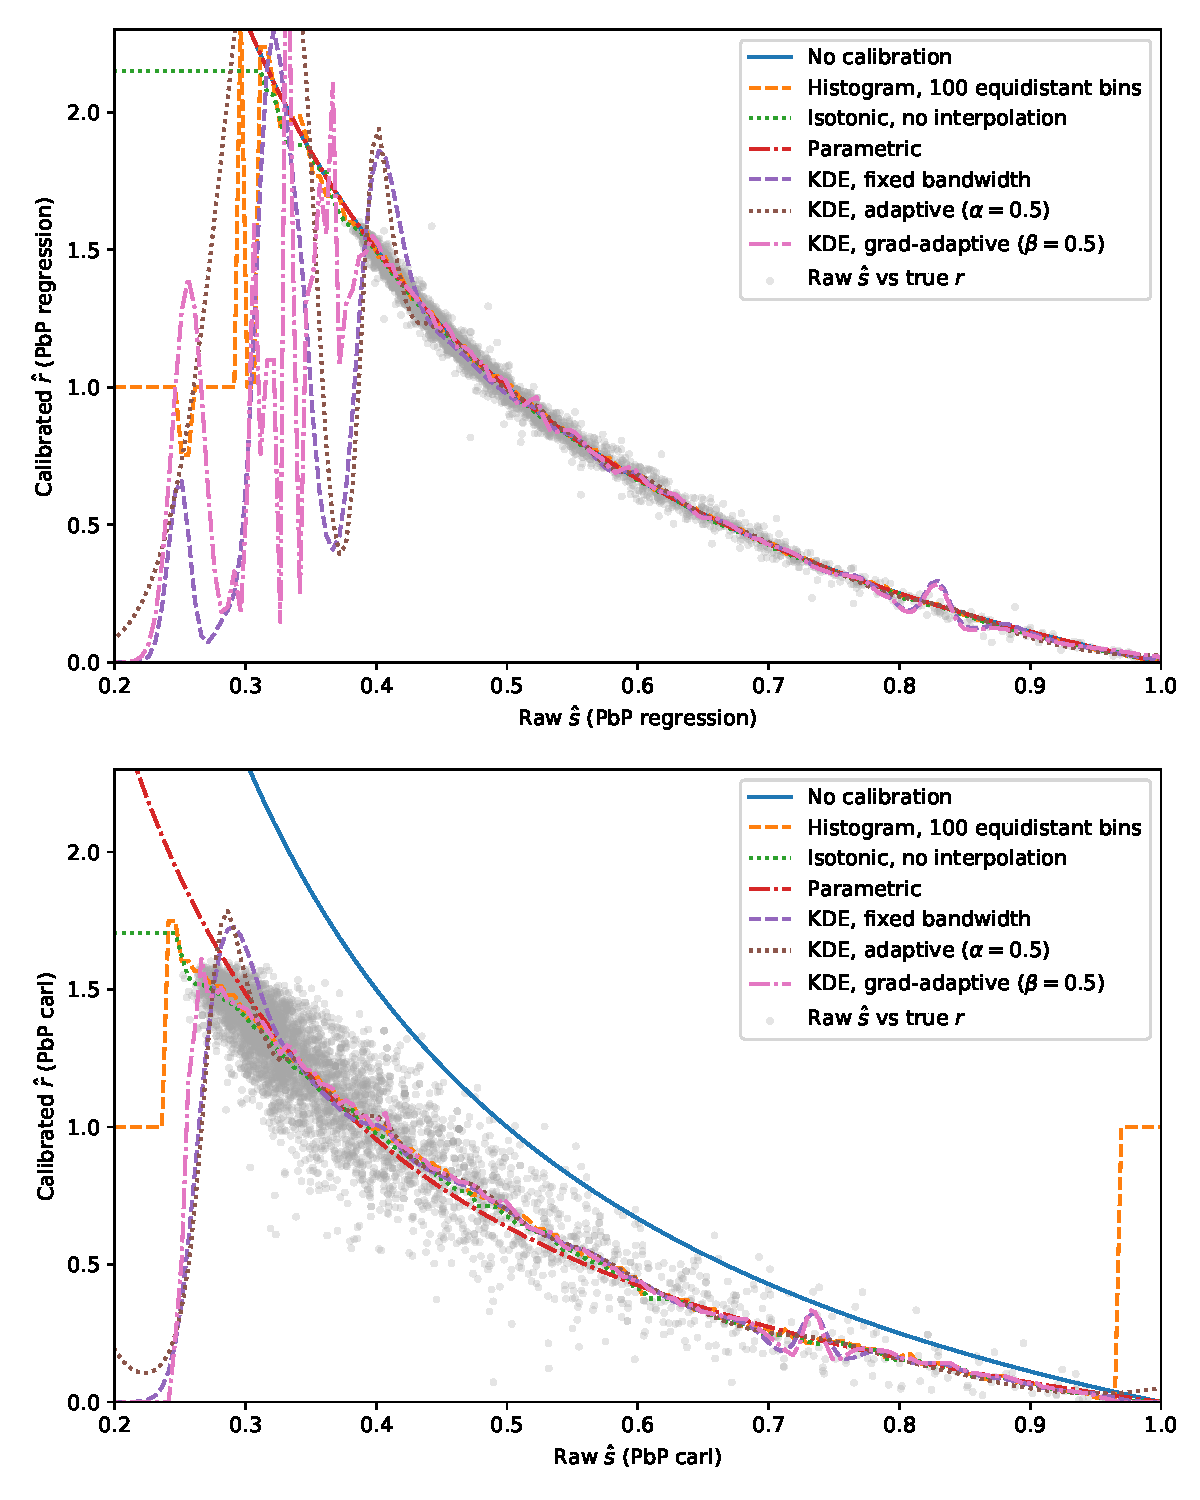
\includegraphics[width=\textwidth]{figures/calibration/calibration_curves.pdf}%
  \caption{Calibration curbes for different calibration strategies.
    Top: point-by-point regression. Bottom: point-by-point carl.}
  \label{fig:calibration_curves}
\end{figure}





%%%%%%%%%%%%%%%%%%%%%%%%%%%%%%%%%%%%%%%%%%%%%%%%%%%%%%%%%%%%
\subsection{Physics-aware setup}
%%%%%%%%%%%%%%%%%%%%%%%%%%%%%%%%%%%%%%%%%%%%%%%%%%%%%%%%%%%%

The physics-aware setup is based on the analytic
form of the morphing weights $w_i (\boldtheta)$. These factors
crucially depend on the basis points in the morphing procedure, as we
show in Figures~\ref{fig:morphing_weights1} and
\ref{fig:morphing_weights2}. Here we stick to the choice
shown in Figure~\ref{fig:morphing_weights2}, which
reduces the weights and the cancellations between them compared to
other basis choices. For now we only analyse the training sample
consisting only of these basis values of $\boldtheta_0$.

\begin{figure}
  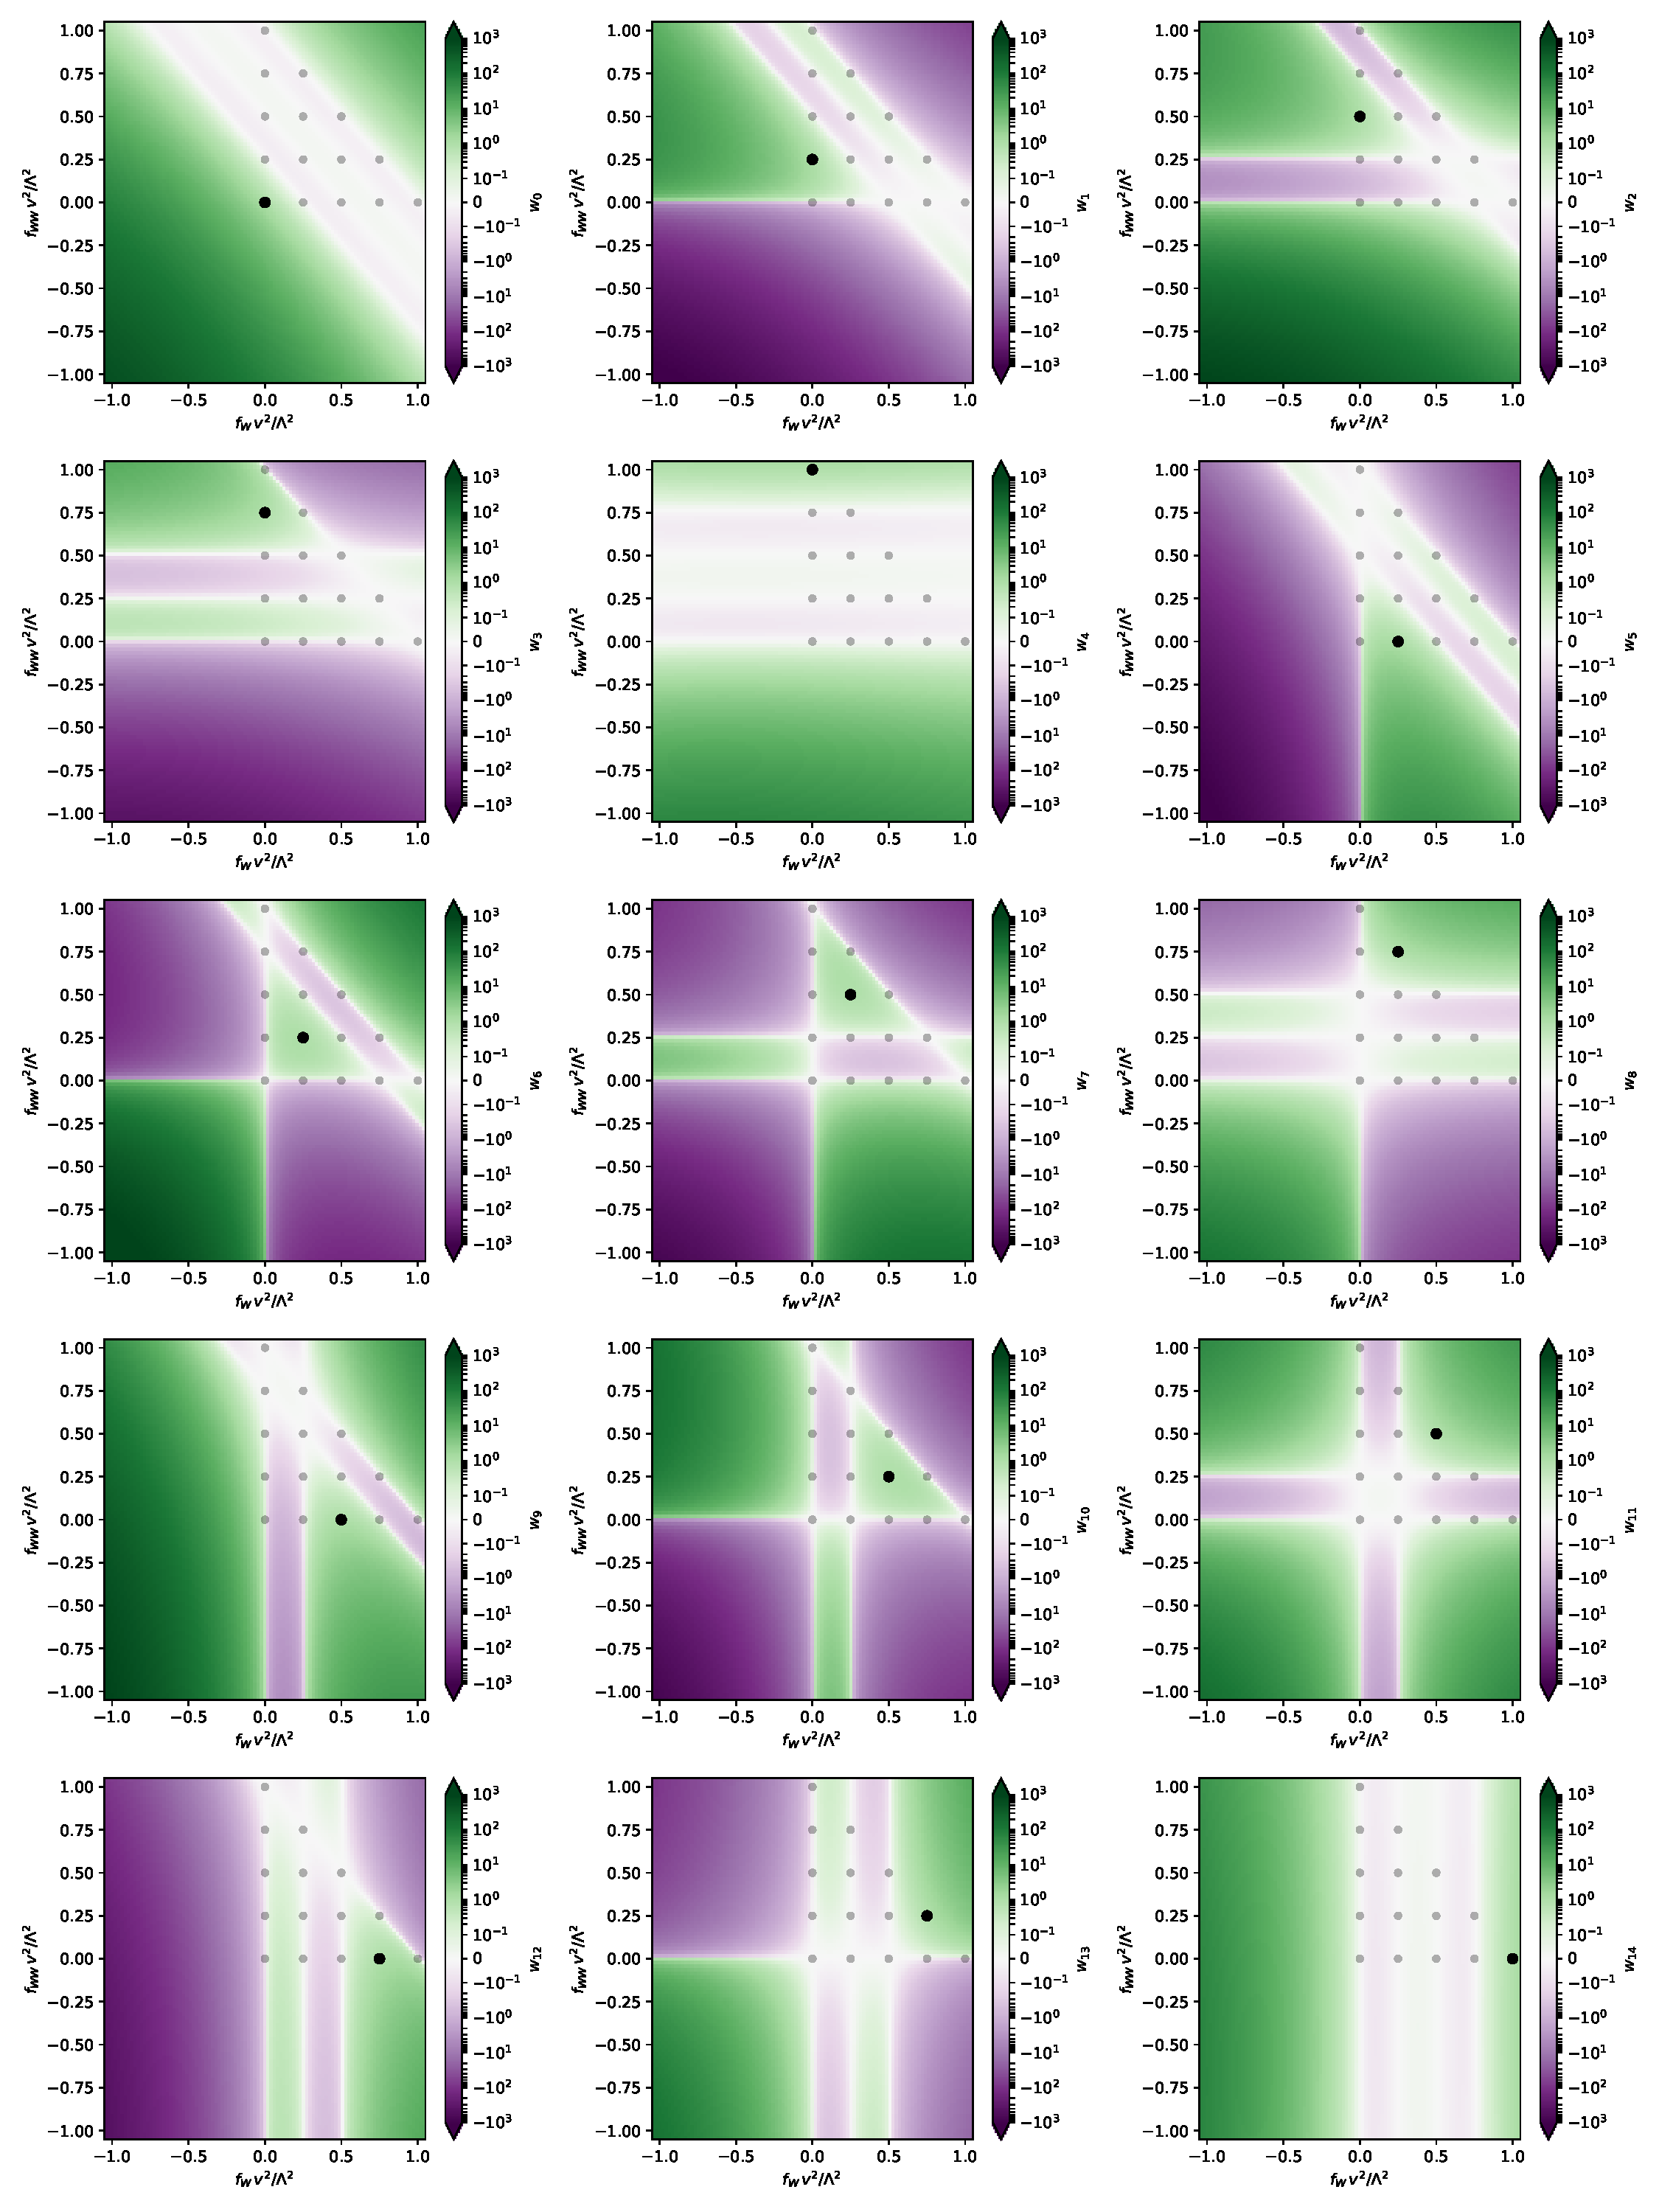
\includegraphics[width=\textwidth]{figures/morphing/morphing_original.pdf}%
  \caption{Morphing weights $w_i(\boldtheta)$ for basis points chosen
    only in one quadrant of the parameter space of interest.}
  \label{fig:morphing_weights1}
\end{figure}

\begin{figure}
  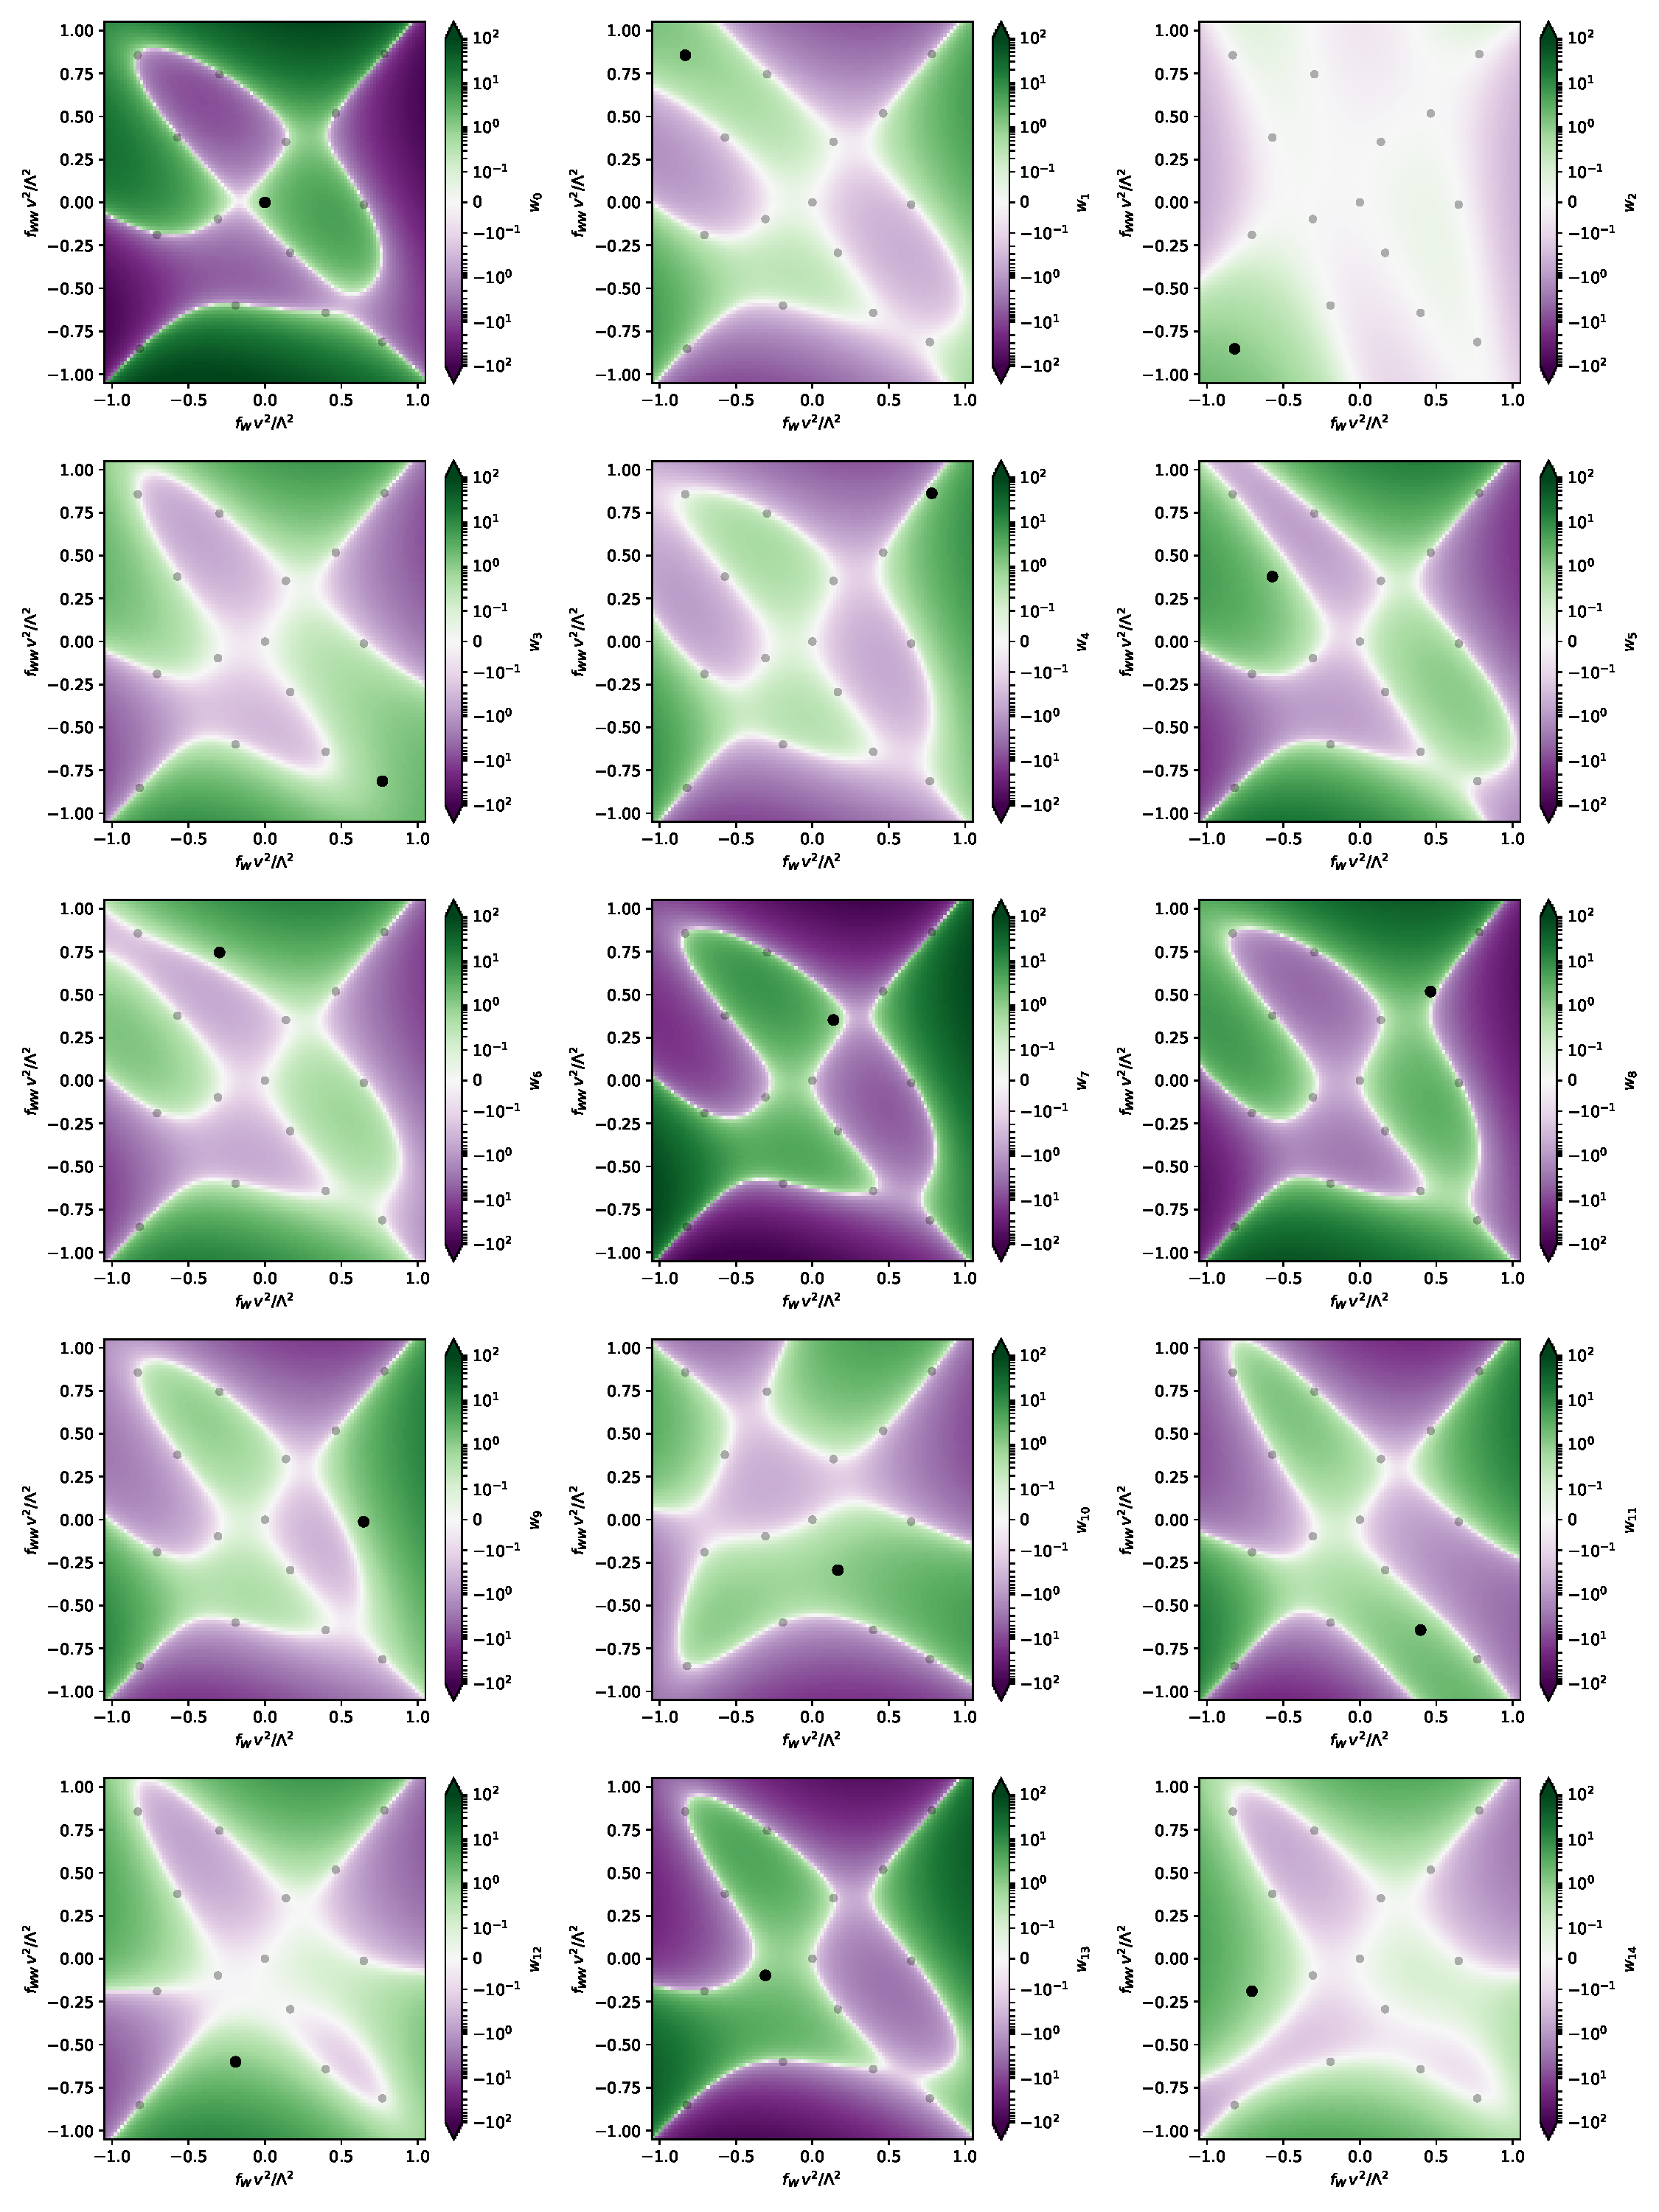
\includegraphics[width=\textwidth]{figures/morphing/morphing_optimized2.pdf}%
  \caption{Morphing weights $w_i(\boldtheta)$ for basis points
    distributed over the full relevant parameter space.}
  \label{fig:morphing_weights2}
\end{figure}

\dots



%%%%%%%%%%%%%%%%%%%%%%%%%%%%%%%%%%%%%%%%%%%%%%%%%%%%%%%%%%%%
\clearpage
\section{Conclusions}
\label{sec:conclusions}
%%%%%%%%%%%%%%%%%%%%%%%%%%%%%%%%%%%%%%%%%%%%%%%%%%%%%%%%%%%%

\dots



%%%%%%%%%%%%%%%%%%%%%%%%%%%%%%%%%%%%%%%%%%%%%%%%%%%%%%%%%%%%

%%%%%%%%%%%%%%%%%%%%%%%%%%%%%%%%%%%%%%%%%%%%%%%%%%%%%%%%%%%%
\clearpage
\appendix
\section{Two-dimensional likelihood}
\label{sec:appendix_2d}
%%%%%%%%%%%%%%%%%%%%%%%%%%%%%%%%%%%%%%%%%%%%%%%%%%%%%%%%%%%%

Instead of estimating the density over the full 15-dimensional
phase-space, we also check some of the approaches on the much simpler
problem of estimating the density of the two-dimensional distribution
$p(p_{T,j1}, \Delta \phi_{jj} ; \boldtheta)$.




%%%%%%%%%%%%%%%%%%%%%%%%%%%%%%%%%%%%%%%%%%%%%%%%%%%%%%%%%%%%
\subsection{Benchmark hypothesis test}
%%%%%%%%%%%%%%%%%%%%%%%%%%%%%%%%%%%%%%%%%%%%%%%%%%%%%%%%%%%%

For two benchmark parameter points
%
\begin{equation}
  \boldtheta_0 = \twovec{-0.2} {-0.2} \,, \quad
  \boldtheta_1 = \twovec{0.2} {0.2}
  \label{eq:pointwise_tuning_benchmarks}
\end{equation}
%
we first analyse how well \toolfont{carl} can estimate the likelihood ratio
%
\begin{equation}
  r(\boldx) = \frac {p(\boldx | \boldtheta_0)}  {p(\boldx | \boldtheta_1)}
  \label{eq:pointwise_tuning_r}
\end{equation}
%
depending on the classifier, its hyperparameters, and a number of
different settings.

For each of the four feature sets outlined above (2D, medium set, full
kinematics, full kinematics plus derived variables), we tune the
parameters in two steps. First, we perform a randomized scan over
the hyperparameters, maximizing the classification power between event
samples sampled from $p(\boldx | \boldtheta_0)$ and
$p(\boldx | \boldtheta_1)$. In a second step we finetune these
parameters on the mean squared error between the \toolfont{carl}
estimate $\log \hat{r}(\boldx)$ and the true value $\log r(\boldx)$.

The first classifier we consider is a \emph{random forest}, more
precisely extremely randomized trees, in the
\toolfont{sklearn.ensemble.ExtraTreesClassifier} implementation. The
following parameters are tuned:
%
\begin{itemize}
  \item \toolfont{n\_estimators}, the number of trees in the forest;
  \item \toolfont{max\_features}, the number of features considered in
    the search for the best split;
  \item \toolfont{max\_depth}, the maximum depth of the trees;
  \item \toolfont{min\_samples\_split}, the minimum fraction of events
    at a node required for a split; and
  \item \toolfont{min\_samples\_leaf}, the minimum fraction of events
    in a leaf.
\end{itemize}

A \emph{multi-layer perceptron} implemented as a
\toolfont{sklearn.neural\_network.MLPClassifier} is our second
classifier. We optimize the following parameters:
%
\begin{itemize}
  \item \toolfont{hidden\_layer\_sizes}, describing the number of hidden
  layers and the number of neurons in each layer;
  \item \toolfont{activation}, the activation function; and
  \item \toolfont{alpha}, an $L^2$ penalty term.
\end{itemize}

For both classifiers, the kinematic features are first rescaled to a
normal distribution with a
\toolfont{sklearn.preprocessing.StandardScaler}.



\begin{figure}
  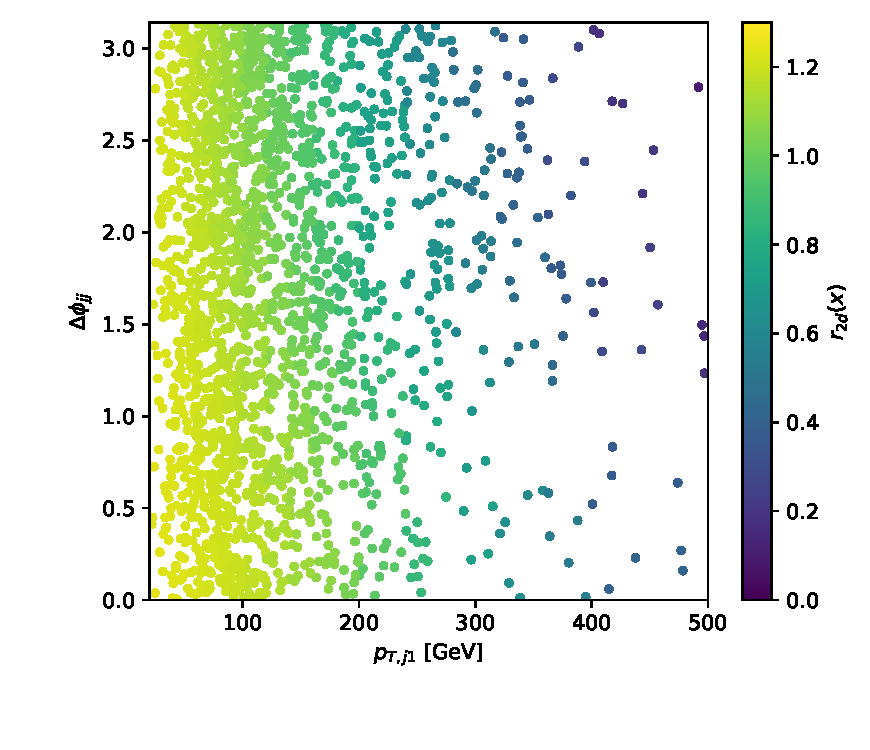
\includegraphics[height=0.45\textwidth]{figures/appendix/pointwise_tuning_2d/r_over_x.pdf}
  \caption{Truth likelihood ratio $r(\boldx)$ as defined in
    \autoref{eq:pointwise_tuning_r} for the 2D case. The effect of the
    binning in the calculation of $r_{\text{2d}}(\boldx)$ is clearly
    visible.}
  \label{fig:pointwise_tuning_2d_r_x}
\end{figure}

First we only consider two kinematic features, the leading jet
momentum and the azimuthal angle between the two
jets. \autoref{fig:pointwise_tuning_2d_r_x} shows how the truth
likelihood ratio between the two points defined in
\autoref{eq:pointwise_tuning_benchmarks} depends on these observables.

\begin{table}
\begin{tabular}{ll rrr}
  \toprule 
  Classifier & Parameter & Range & Good & Best \\
  \midrule
  Random forest & \toolfont{n\_estimators} & $50 \dots 200$ & $50 \dots 200$  & $100$ \\
  & \toolfont{max\_features} & $1, 2$ & $2$ & $2$ \\
  & \toolfont{max\_depth} & $1 \dots 20, \infty$ & $6\dots 8$ & $8$ \\
  & \toolfont{min\_samples\_split} & $0 \dots 1$ & $10^{-4} \dots 10^{-3}$ & $10^{-3}$ \\
  & \toolfont{min\_samples\_leaf} & $0 \dots 0.5$ & $0$ & $0$ \\
  \midrule
  Neural network & number of hidden layers & $1,2,3$ & $2$ & $2$\\
  & neurons at each layer & $2\dots 20$ per layer & $(20,20)$ & $(20,20)$\\
  & activation function & $\tanh, \relu, \logistic$ & $\tanh, \relu$ & $\tanh$ \\
  & $\alpha$ & $0\dots 100$ & $0\dots 1$ & $10^{-3}$\\
  \bottomrule
\end{tabular}
\caption{Hyperparameter scan on the classification problem between
  $\boldtheta_0$ and $\boldtheta_1$ for the 2D case. For both classifier
  and each parameter we show the considered range, the range of values
  with good results (\ie ROC AUC close to the optimum),
  and the (rounded) optimal value. }
 \label{tbl:pointwise_tuning_2d_parameters}
\end{table}

We first tune hyperparameters with a randomized scan on the
classification problem between unweighted event samples drawn from
$p(\boldx | \boldtheta_0)$ and $p(\boldx | \boldtheta_1)$. Using
\toolfont{sklearn.model\_selection.RandomizedSearchCV}, we optimize on
the ROC AUC. We give the optimal parameters in
\autoref{tbl:pointwise_tuning_2d_parameters}. Key to a good
performance for the random forest is a maximal depth around 8. Only
considering one feature at each splitting or requiring a large number
of events for a splitting or at each leaf lead to a worse
performance. Above a certain threshold, the number of trees does not
have a huge effect. For the neural network, two hidden layers with 20
neurons each and tanh or ReLU activation functions perform best, while
the value of the regulator $\alpha$ is not very important.

\begin{figure}
  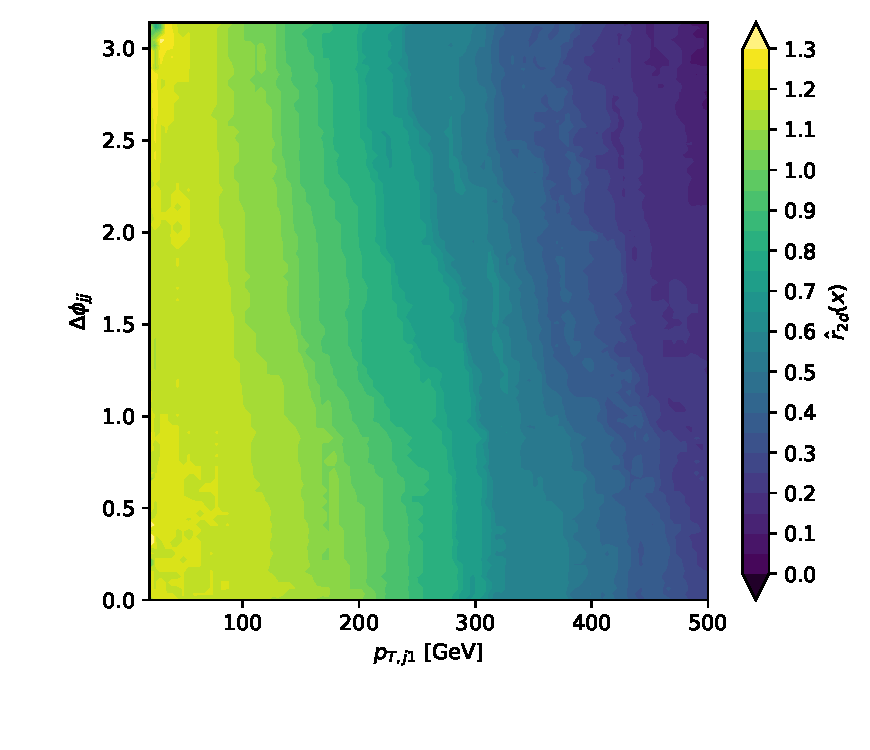
\includegraphics[height=0.45\textwidth]{figures/appendix/pointwise_tuning_2d/rhat_over_x_grid_rf.pdf}%
  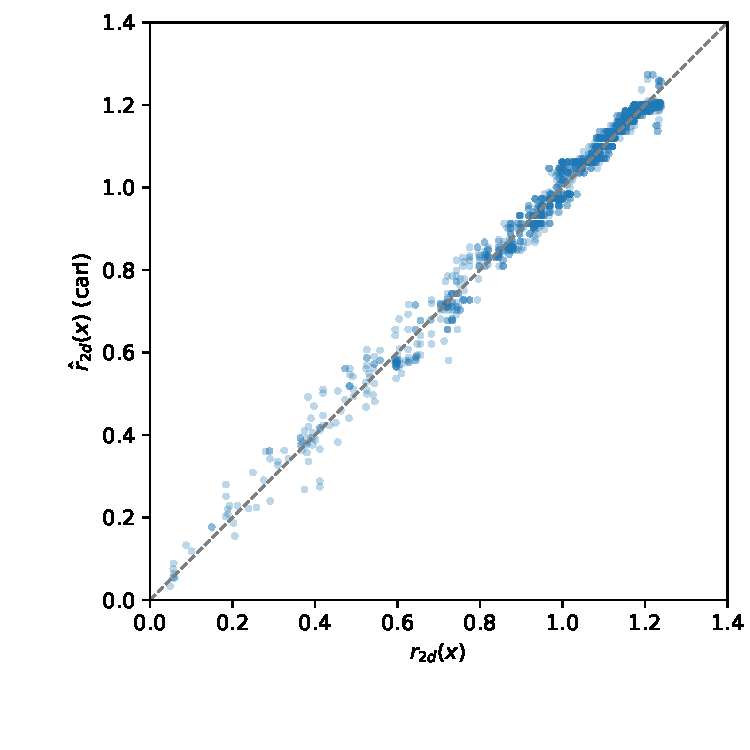
\includegraphics[height=0.45\textwidth]{figures/appendix/pointwise_tuning_2d/rhat_vs_r_rf.pdf}%
  \caption{Likelihood ratio estimation with the tuned random forest
    for the 2D case. Left: Distribution of
    \toolfont{carl}'s estimate $\hat{r}(\boldx)$ as a function of the
    observables. Right: scatter plot between the true $r(\boldx)$ and
    the estimate $\hat{r}(\boldx)$}.
  \label{fig:pointwise_tuning_2d_rf_performance}
\end{figure}

\begin{figure}
  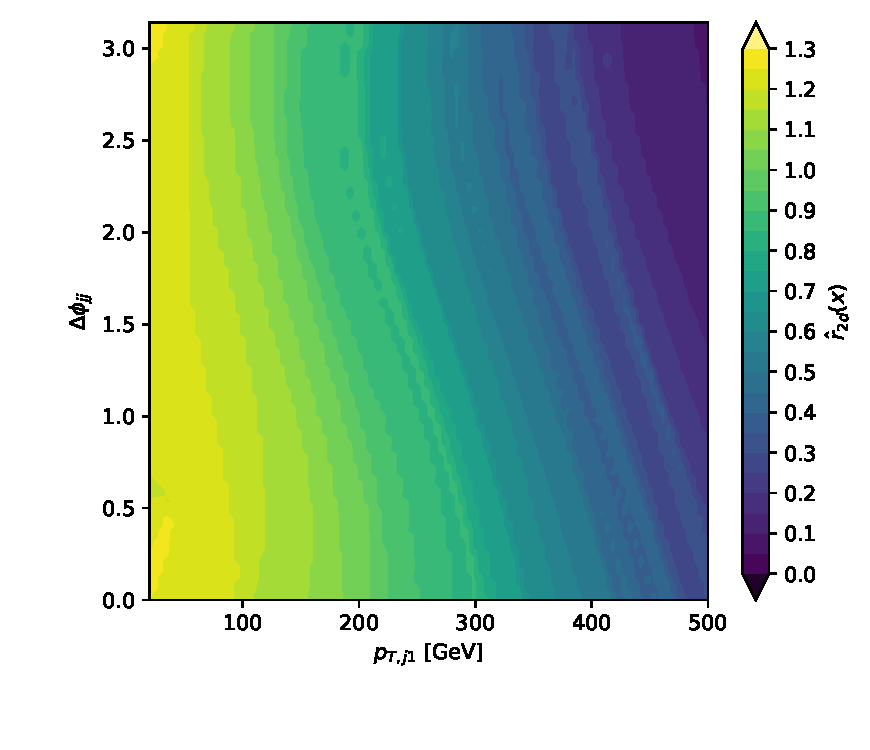
\includegraphics[height=0.45\textwidth]{figures/appendix/pointwise_tuning_2d/rhat_over_x_grid_mlp.pdf}
  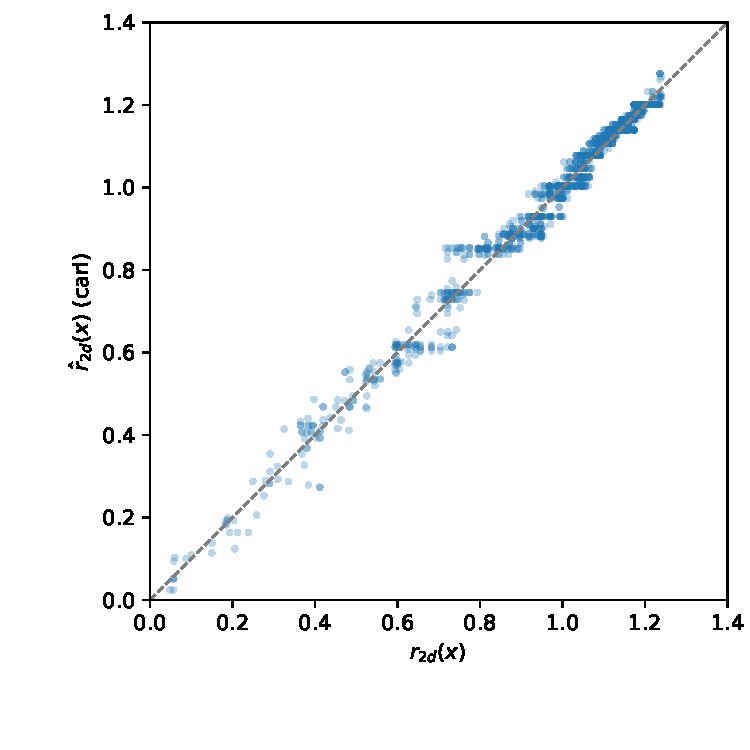
\includegraphics[height=0.45\textwidth]{figures/appendix/pointwise_tuning_2d/rhat_vs_r_mlp.pdf}
  \caption{Likelihood ratio estimation with the tuned neural network
    for the 2D case. Left: Distribution of
    \toolfont{carl}'s estimate $\hat{r}(\boldx)$ as a function of the
    observables. Right: scatter plot between the true $r(\boldx)$ and
    the estimate $\hat{r}(\boldx)$}.
  \label{fig:pointwise_tuning_2d_mlp_performance}
\end{figure}

In Figures~\ref{fig:pointwise_tuning_2d_rf_performance} and
\ref{fig:pointwise_tuning_2d_mlp_performance} we show how well
\toolfont{carl} can estimate the true likelihood ratio $r(\boldx)$
with the tuned classifiers given in the right column of
\autoref{tbl:pointwise_tuning_2d_parameters}.

Next, we vary all parameters one by one and see how this affects the
mean squared error of $\log \hat{r}(\boldx)$. The results are shown in
Figures~\ref{fig:pointwise_tuning_2d_rf_tuning} to
\ref{fig:pointwise_tuning_2d_carl_tuning}.

\begin{figure}
  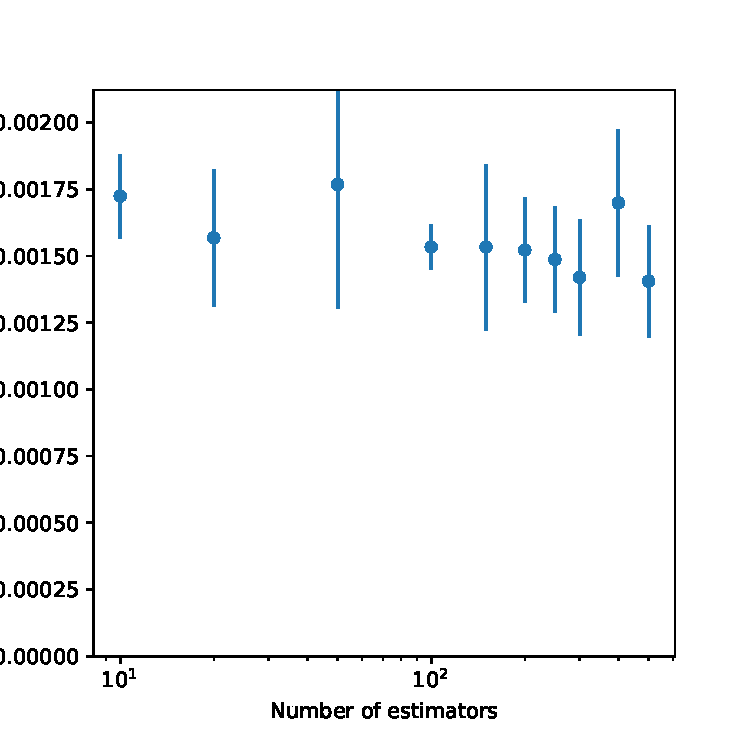
\includegraphics[width=0.45\textwidth]{figures/appendix/pointwise_tuning_2d/mse_rf_n_estimators.pdf}%
  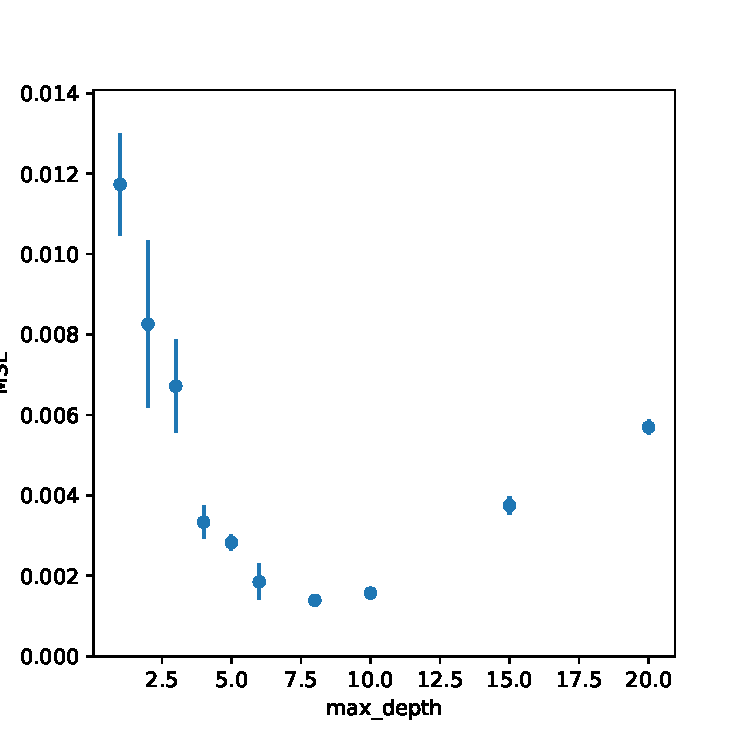
\includegraphics[height=0.45\textwidth]{figures/appendix/pointwise_tuning_2d/mse_rf_max_depths.pdf}\\%
  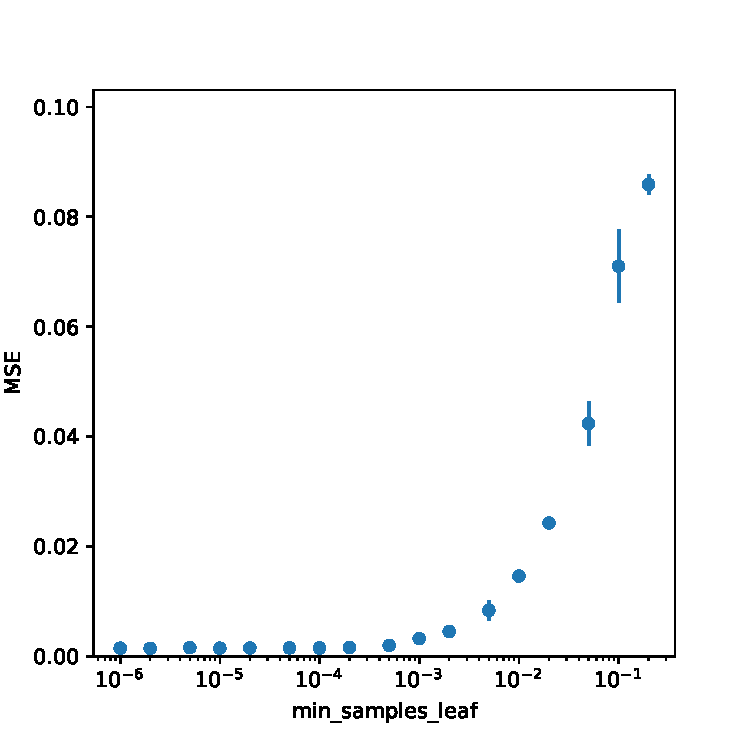
\includegraphics[height=0.45\textwidth]{figures/appendix/pointwise_tuning_2d/mse_rf_min_samples_leaf.pdf}%
  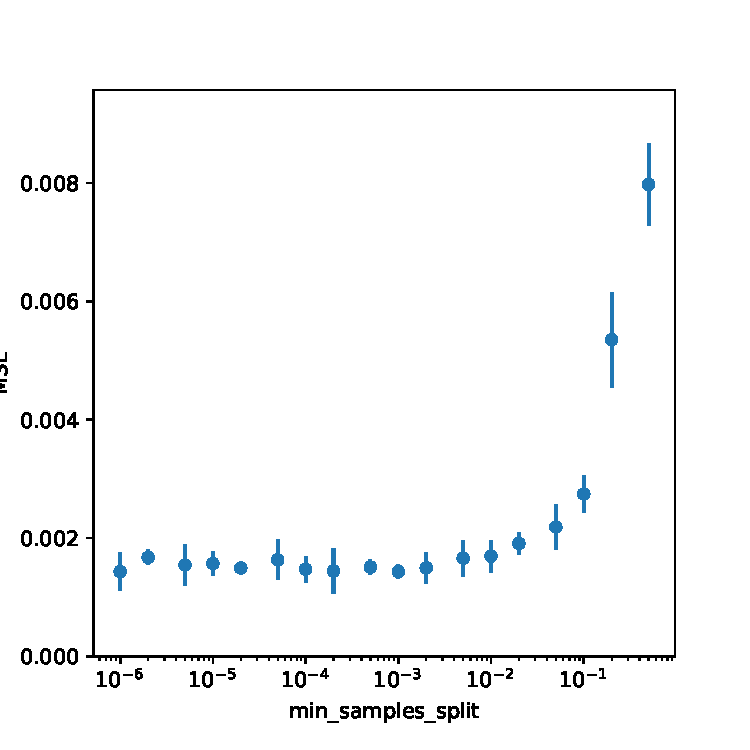
\includegraphics[height=0.45\textwidth]{figures/appendix/pointwise_tuning_2d/mse_rf_min_samples_splits.pdf}%
  \caption{carl performance as a function of the random forest
    hyperparameters. We show the mean squred error of the estimated
    log likelihood ratio between two benchmark points for the 2D
    case. Each data point shows the mean of five calculations, the
    error bars are $95\%$ confidence intervals.}
  \label{fig:pointwise_tuning_2d_rf_tuning}
\end{figure}

\begin{figure}
  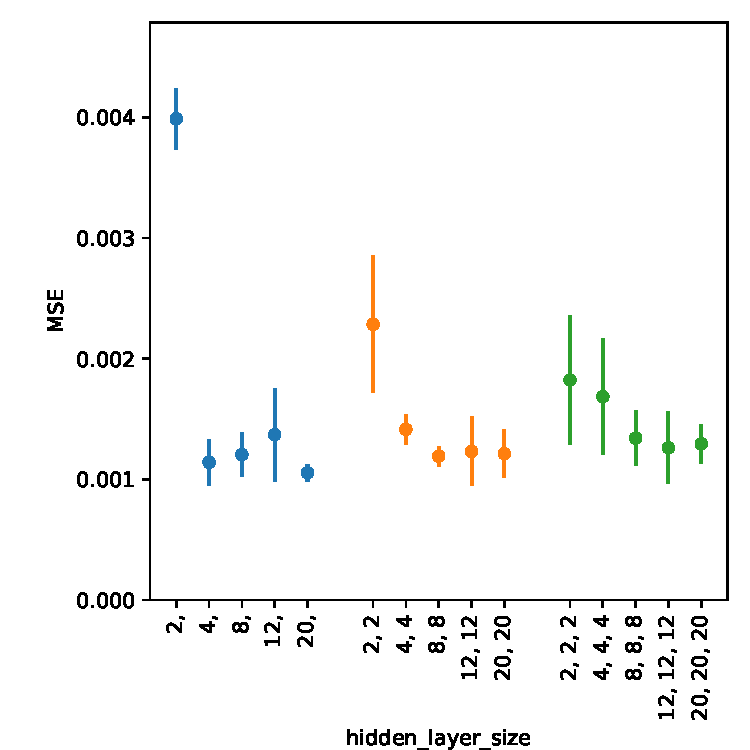
\includegraphics[width=0.45\textwidth]{figures/appendix/pointwise_tuning_2d/mse_mlp_hidden_layer_sizes.pdf}%
  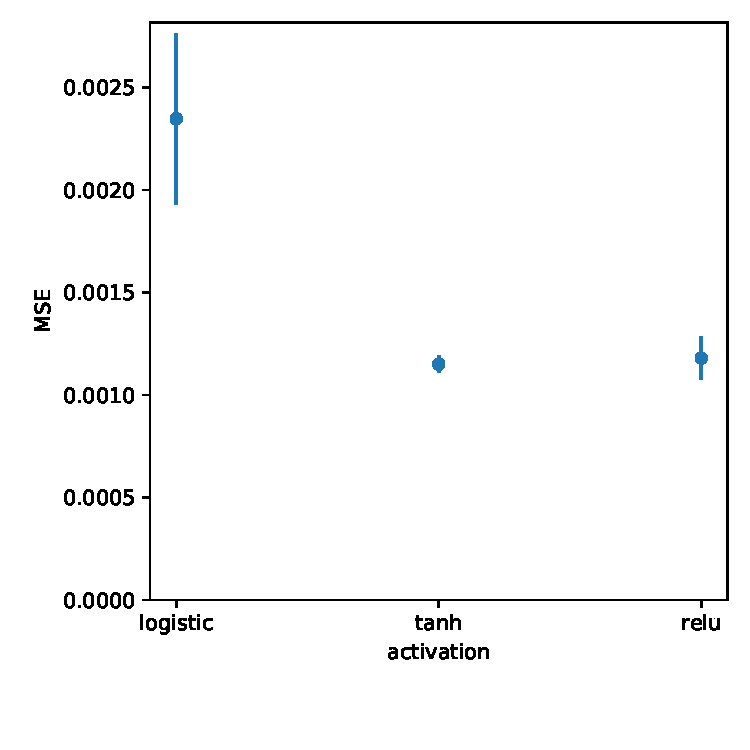
\includegraphics[height=0.45\textwidth]{figures/appendix/pointwise_tuning_2d/mse_mlp_activation.pdf}\\%
  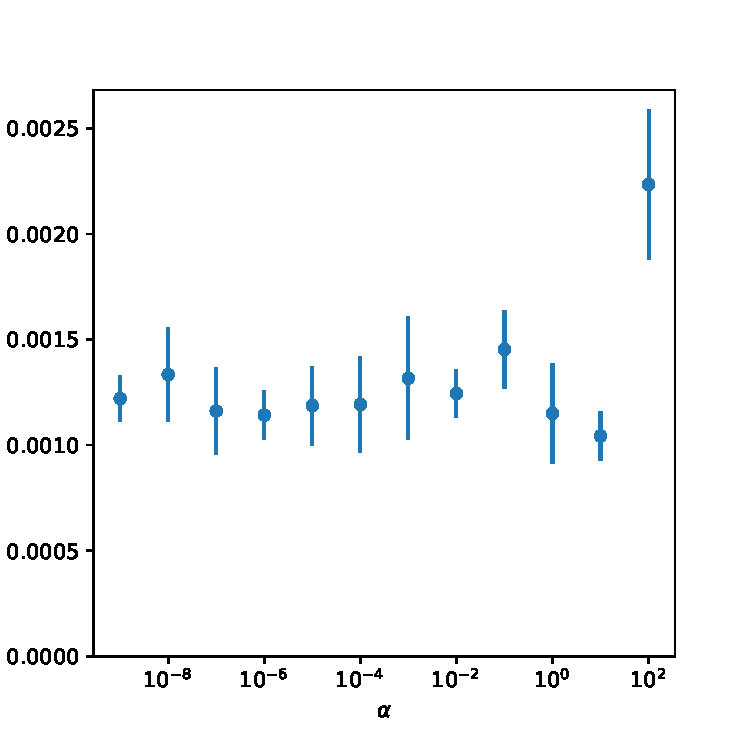
\includegraphics[height=0.45\textwidth]{figures/appendix/pointwise_tuning_2d/mse_mlp_alpha.pdf}%
  \caption{carl performance as a function of the neural network
    hyperparameters. Mean squred error of the estimated log likelihood
    ratio between two benchmark points for the 2D case. Each data
    point shows the mean of five calculations, the error bars are
    $95\%$ confidence intervals.}
  \label{fig:pointwise_tuning_2d_mlp_tuning}
\end{figure}

The parameters that are best for the classification problem also work
best for the estimation of the likelihood ratio with
$\toolfont{carl}$. The performance of the random forest crucially
depends on the maximal depth, while the neural network works well with
pretty much any setup, as long as each layer has enough neurons. To
reduce training time, we therefore define a final setup of the neural
network with a reduced number of 8 neurons in each hidden layer. For
the random forest, we stick to the parameters in the right column of
\autoref{tbl:pointwise_tuning_2d_parameters}.

\begin{figure}
  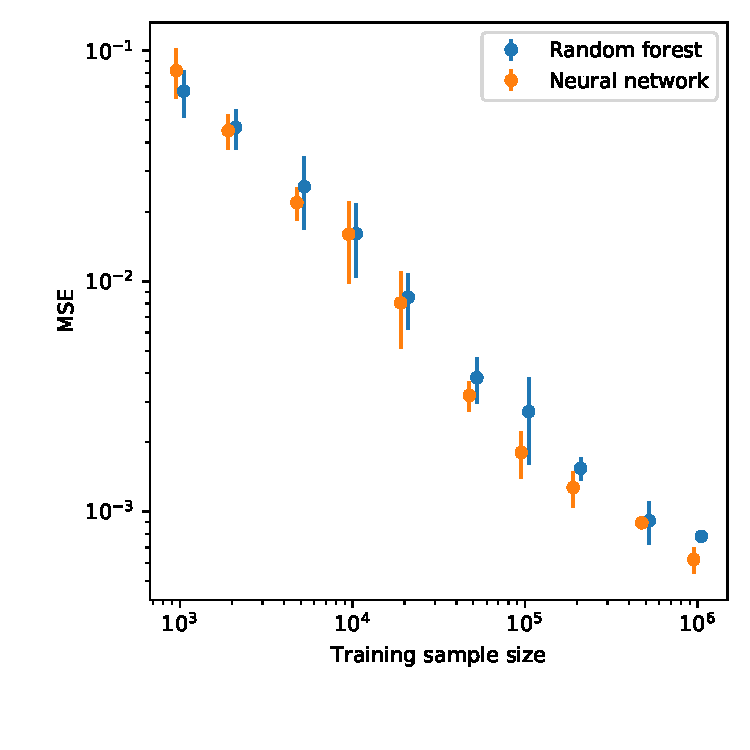
\includegraphics[width=0.45\textwidth]{figures/appendix/pointwise_tuning_2d/mse_training_sample_size.pdf}%
  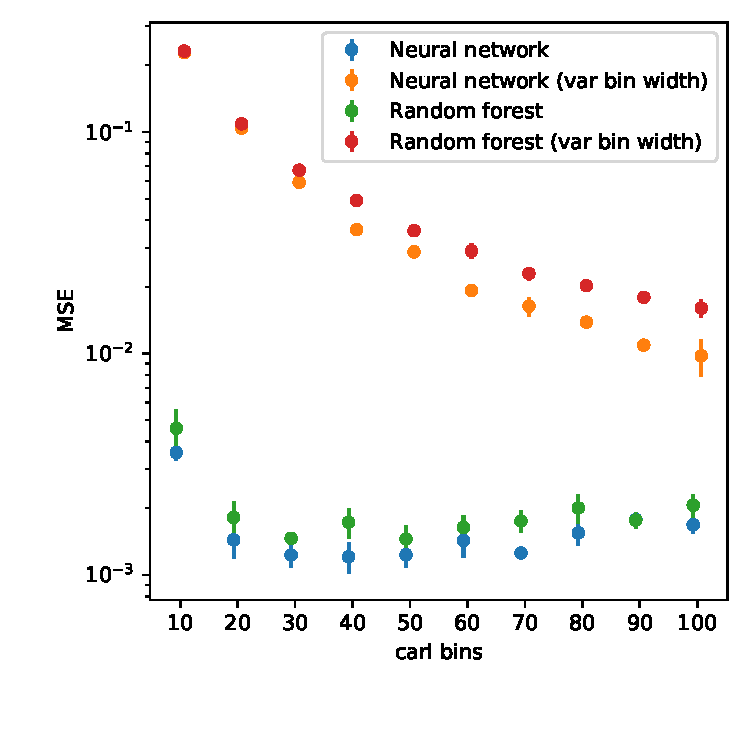
\includegraphics[height=0.45\textwidth]{figures/appendix/pointwise_tuning_2d/mse_carl_bins.pdf}%
  \caption{carl performance as a function of the training sample size
    (left) and the number of bins in the \toolfont{carl} calibration
    histograms.  We show the mean squred error of the estimated log
    likelihood ratio between two benchmark points for the 2D
    case. Each data point shows the mean of five calculations, the
    error bars are $95\%$ confidence intervals.}
  \label{fig:pointwise_tuning_2d_carl_tuning}
\end{figure}

\autoref{fig:pointwise_tuning_2d_carl_tuning} shows the effect of the
size of the training samples as well as the binning of \toolfont{carl}'s
calibration histograms.  Regardless of the problematic distribution of
weights in the input samples, the performance becomes much better
with larger training samples. We pick a size of 200\,000 events as a
balance between computation time and performance. The calibration
histograms should have at least 20 bins, and variable bin widths do not
seem to work well at all.

\begin{figure}
  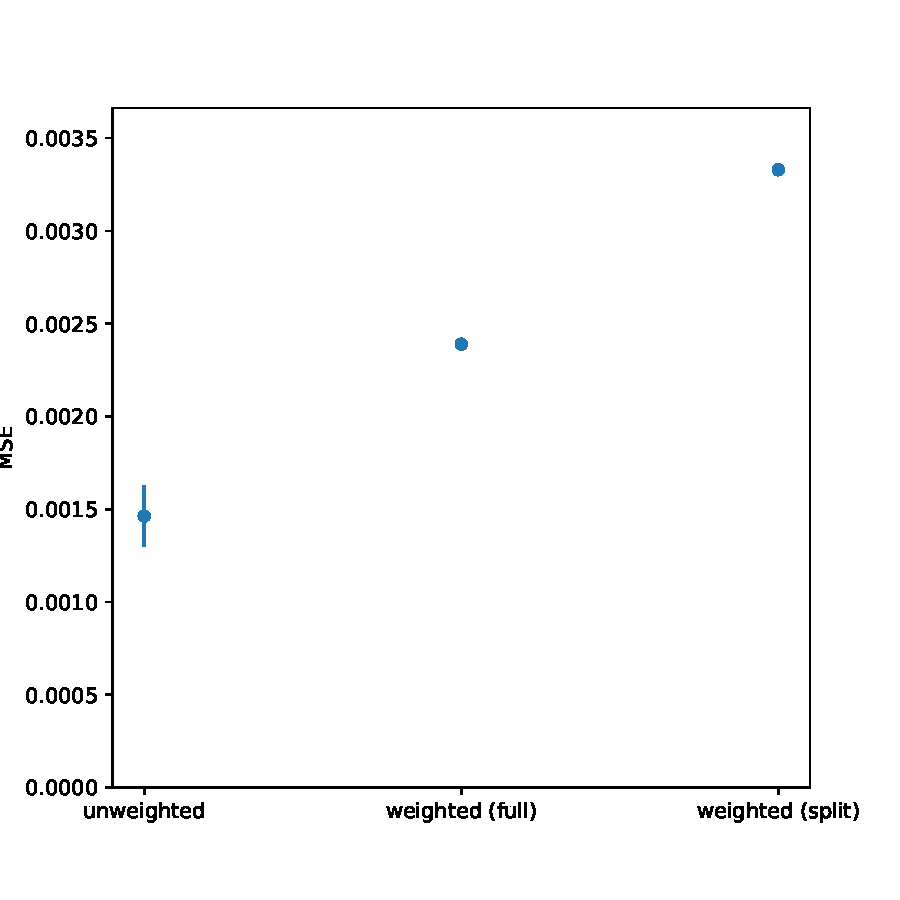
\includegraphics[height=0.45\textwidth]{figures/appendix/pointwise_tuning_2d/mse_weighted_events.pdf}%
  \caption{carl performance with weighted training samples. We show
    the mean squred error of the estimated log likelihood ratio between
    two benchmark points based on the two-dimensional feature
    space.}
  \label{fig:pointwise_tuning_2d_weighted}
\end{figure}

As demonstrated in \autoref{fig:pointwise_tuning_2d_weighted},
training random forests with weighted samples does not improve the
performance, even if the full training sample of 5 million events is
used. However, we did not try to tune the random forest parameters
with weighted input.

\begin{figure}
  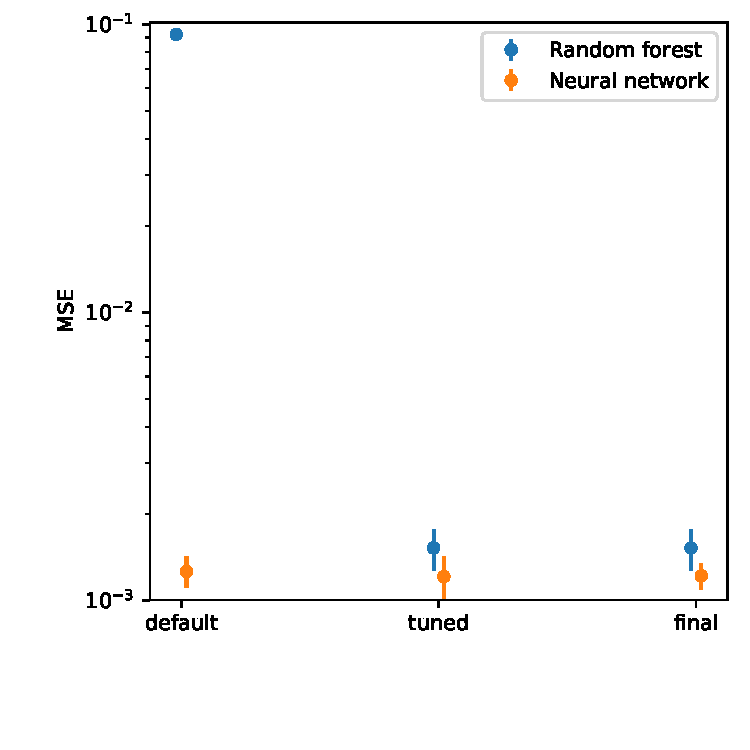
\includegraphics[height=0.45\textwidth]{figures/appendix/pointwise_tuning_2d/mse_final.pdf}%
  \caption{carl performance for the 2D case with \toolfont{sklearn}
    default hyperparameters, the best parameters according to the
    initial hyperparameter scan, and the final parameters as defined
    in the text. We show the mean squred error of the estimated log
    likelihood ratio between two benchmark points. Each data point
    shows the mean of five calculations, the error bars are $95\%$
    confidence intervals.}
  \label{fig:pointwise_tuning_2d_final}
\end{figure}

We summarise \toolfont{carl}'s performance before and after tuning and
compare the two classifiers in
\autoref{fig:pointwise_tuning_2d_final}. We find that the neural
network performs slightly better, and is much less dependent on the
choice of parameters. The output of \toolfont{carl} with this final
neural network setup is shown in
\autoref{fig:pointwise_tuning_2d_final_performance}. As a matter of
fact, the smooth neural net output might be closer to the real
likelihood ratio than our calculated $r(\boldx)$ with its binning
artefacts.

\begin{figure}
  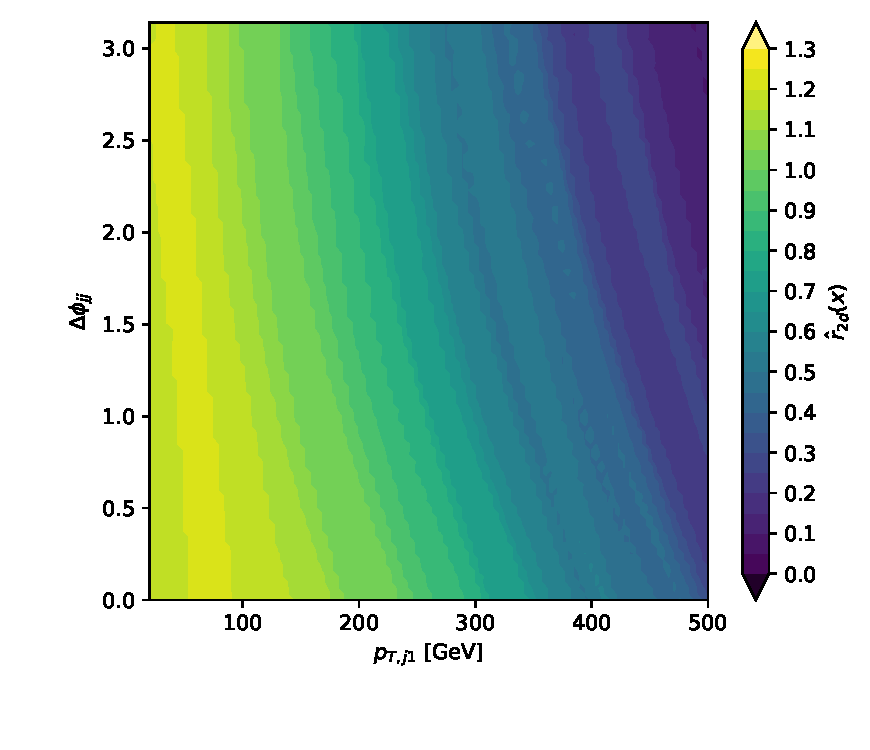
\includegraphics[height=0.45\textwidth]{figures/appendix/pointwise_tuning_2d/rhat_over_x_grid_final.pdf}
  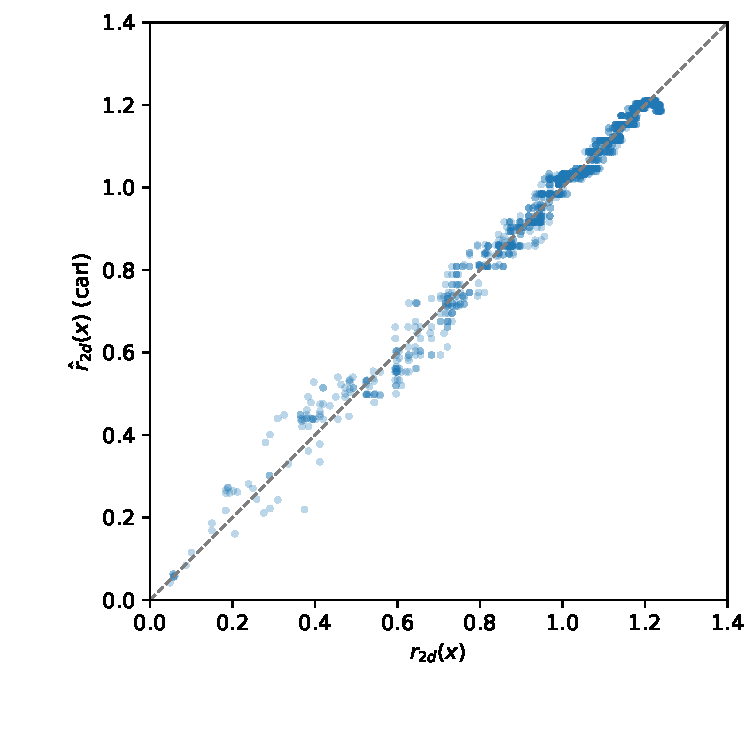
\includegraphics[height=0.45\textwidth]{figures/appendix/pointwise_tuning_2d/rhat_vs_r_final.pdf}
  \caption{Likelihood ratio estimation with the final neural network
    for the 2D case. Left: Distribution of \toolfont{carl}'s estimate
    $\hat{r}(\boldx)$ as a function of the observables. Right: scatter
    plot between the true $r(\boldx)$ and the estimate
    $\hat{r}(\boldx)$}.
  \label{fig:pointwise_tuning_2d_final_performance}
\end{figure}






%%%%%%%%%%%%%%%%%%%%%%%%%%%%%%%%%%%%%%%%%%%%%%%%%%%%%%%%%%%%
\subsection{Validation}
%%%%%%%%%%%%%%%%%%%%%%%%%%%%%%%%%%%%%%%%%%%%%%%%%%%%%%%%%%%%

After tuning the parameters for one specific choice of benchmark
points, we now check how well these settings work for the likelihood ratio
between two different benchmark points
%
\begin{equation}
  \boldtheta_0' = \twovec{0.5} {-0.5} \,, \quad
  \boldtheta_1' = \twovec{-0.5} {0.5} \,.
  \label{eq:pointwise_validation_benchmarks}
\end{equation}

\begin{figure}
  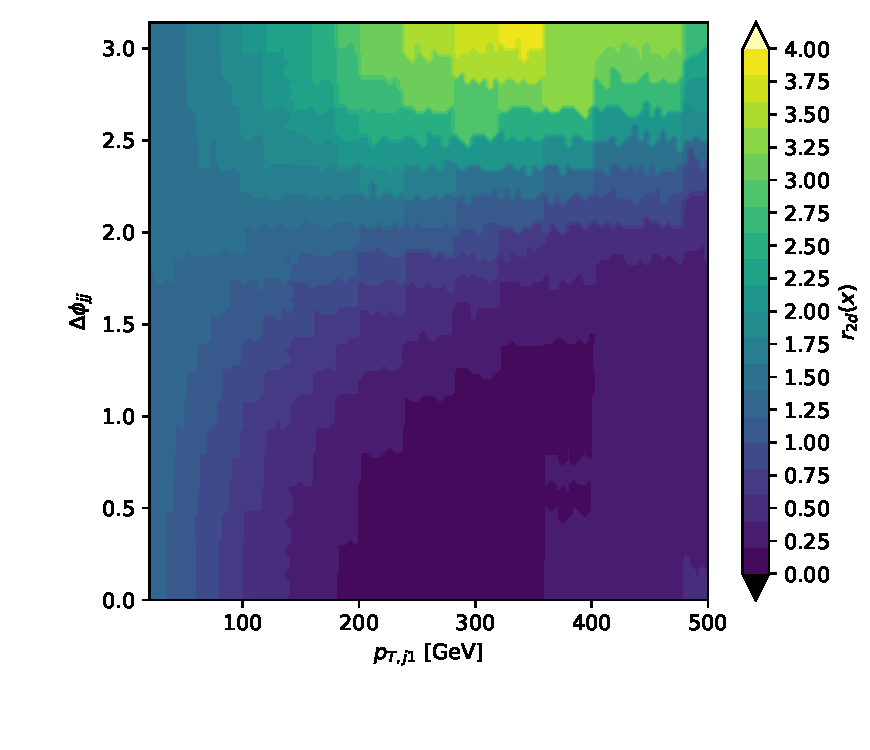
\includegraphics[height=0.45\textwidth]{figures/appendix/pointwise_tuning_2d/r_over_x_grid_alt.pdf}
  \caption{Truth likelihood ratio $r(\boldx)$ between the validation
    benchmark points for the 2D case as a function of the
    observables.}
  \label{fig:pointwise_validation_2d_r_x}
\end{figure}

\autoref{fig:pointwise_validation_2d_r_x} shows the truth likelihood
ratio between the validation benchmark points of
\autoref{eq:pointwise_validation_benchmarks} as a function of the two
observables.

\begin{figure}
  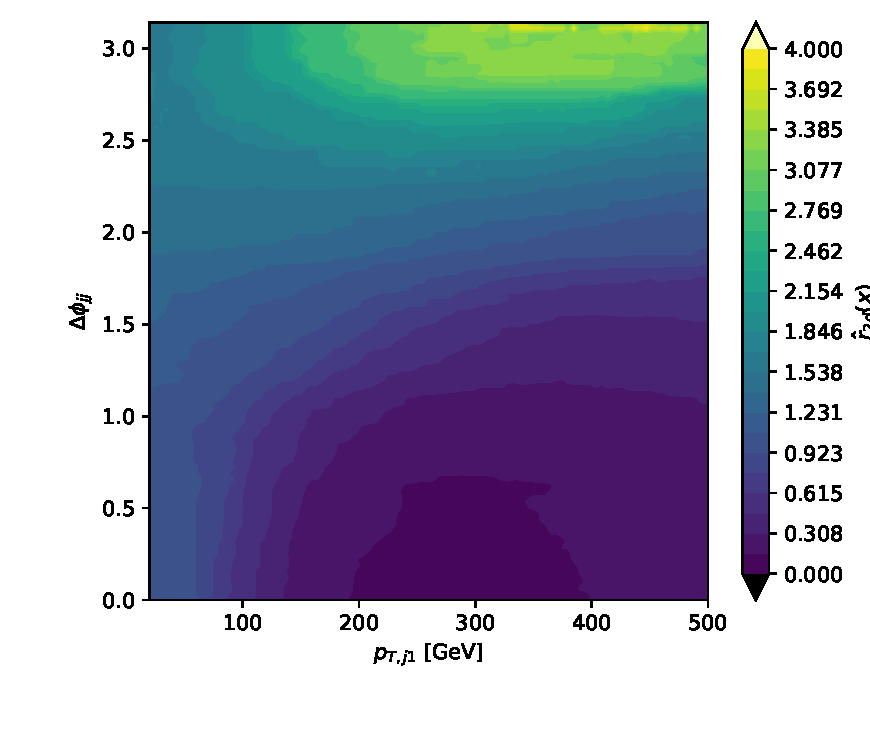
\includegraphics[height=0.45\textwidth]{figures/appendix/pointwise_tuning_2d/rhat_over_x_grid_rf_alt.pdf}%
  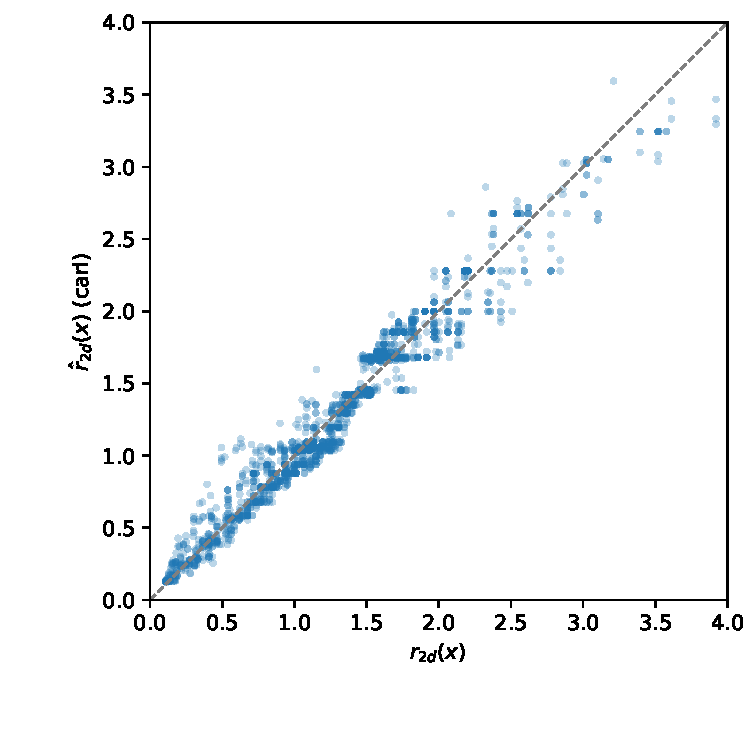
\includegraphics[height=0.45\textwidth]{figures/appendix/pointwise_tuning_2d/rhat_vs_r_rf_alt.pdf}%
  \caption{Likelihood ratio estimation with the tuned random forest on
    separate validation hypotheses for the 2D case. Left: Distribution
    of \toolfont{carl}'s estimate $\hat{r}(\boldx)$ as a function of
    the observables. Right: scatter plot between the true $r(\boldx)$
    and the estimate $\hat{r}(\boldx)$}.
  \label{fig:pointwise_validation_2d_rf_performance}
\end{figure}

\begin{figure}
  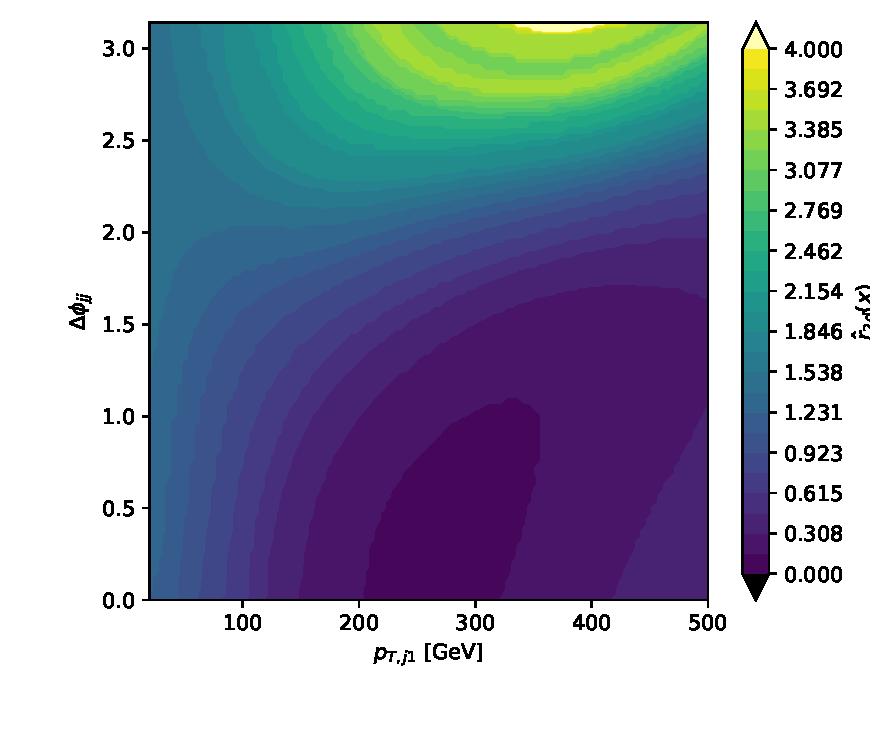
\includegraphics[height=0.45\textwidth]{figures/appendix/pointwise_tuning_2d/rhat_over_x_grid_final_alt.pdf}
  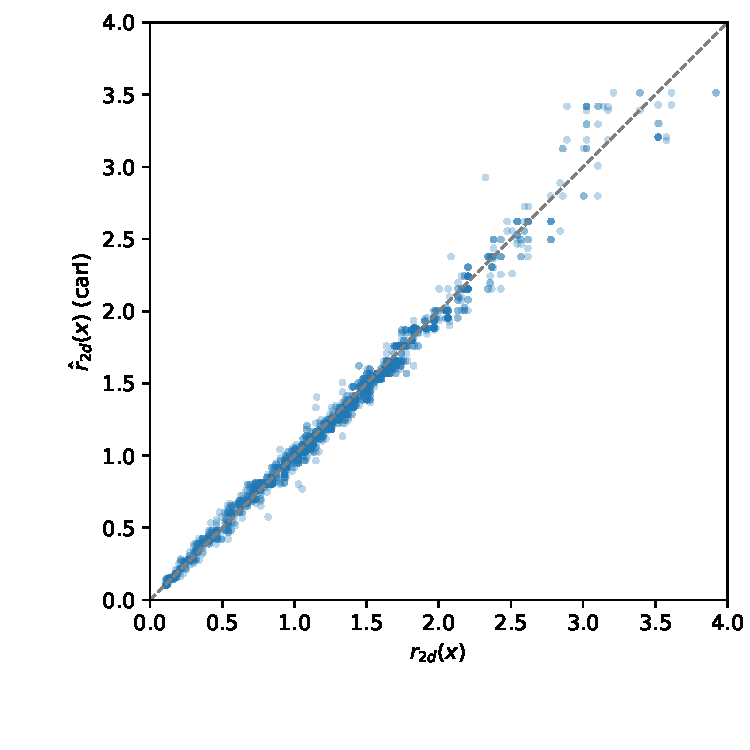
\includegraphics[height=0.45\textwidth]{figures/appendix/pointwise_tuning_2d/rhat_vs_r_final_alt.pdf}
  \caption{Likelihood ratio estimation with the neural network on
    separate validation hypotheses for the 2D case.  Left:
    Distribution of \toolfont{carl}'s estimate $\hat{r}(\boldx)$ as a
    function of the observables. Right: scatter plot between the true
    $r(\boldx)$ and the estimate $\hat{r}(\boldx)$}.
  \label{fig:pointwise_validation_2d_mlp_performance}
\end{figure}

\begin{figure}
  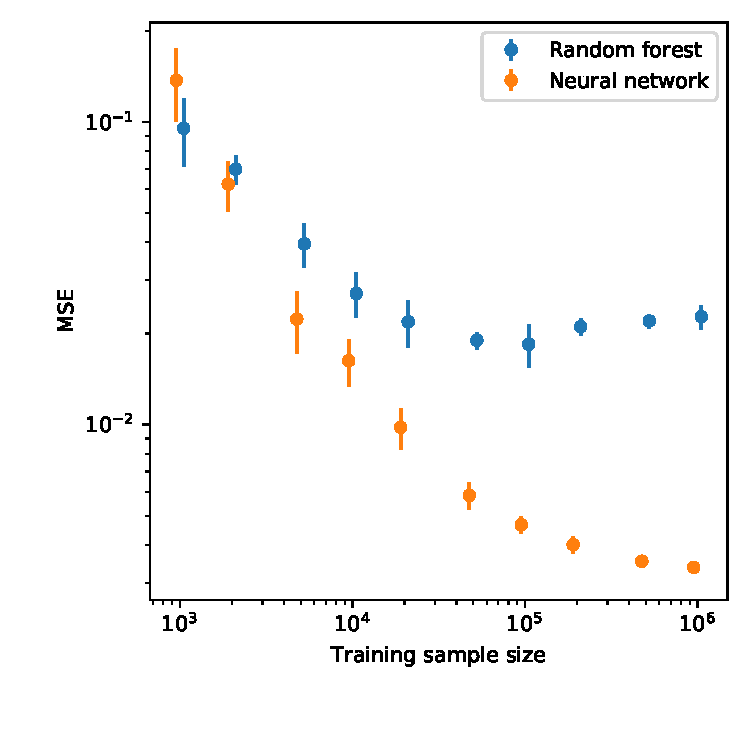
\includegraphics[height=0.45\textwidth]{figures/appendix/pointwise_tuning_2d/mse_training_sample_size_alt.pdf}
  %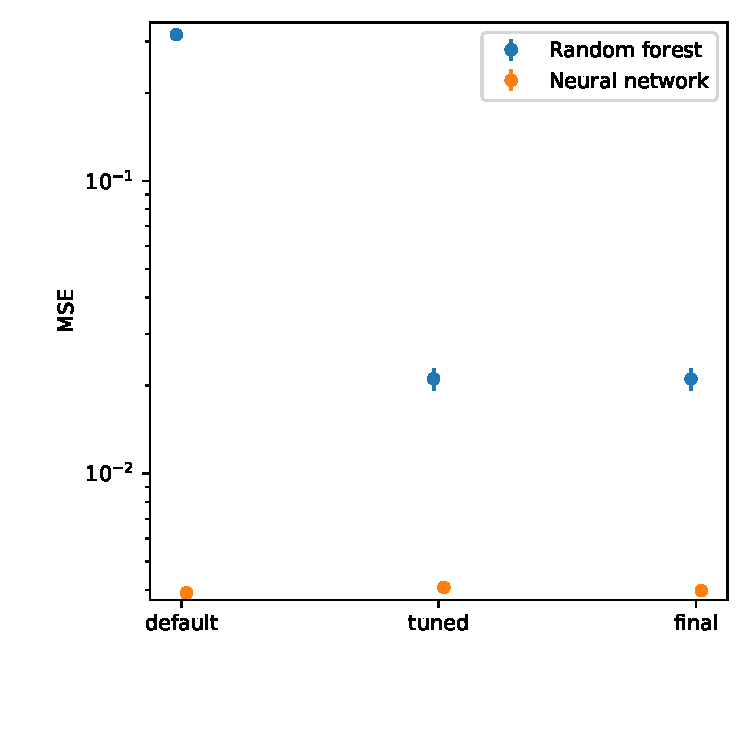
\includegraphics[height=0.45\textwidth]{figures/appendix/pointwise_tuning_2d/mse_final_alt.pdf}
  \caption{carl performance on the validation hypotheses for different
    training sample sizes and classifiers).  We show the mean squred
    error of the estimated log likelihood ratio between two validation
    benchmark points for the 2D case. Each data point shows the mean
    of five calculations, the error bars are $95\%$ confidence
    intervals.}
  \label{fig:pointwise_validation_2d_overview}
\end{figure}

In Figures~\ref{fig:pointwise_validation_2d_rf_performance} to
\ref{fig:pointwise_validation_2d_overview} we show
\toolfont{carl}'s estimation based on the final settings tuned in
the previous section. How this performance depends on the
choice of hyperparameters is illustrated in
\autoref{fig:pointwise_validation_2d_tuning}.

\begin{figure}
  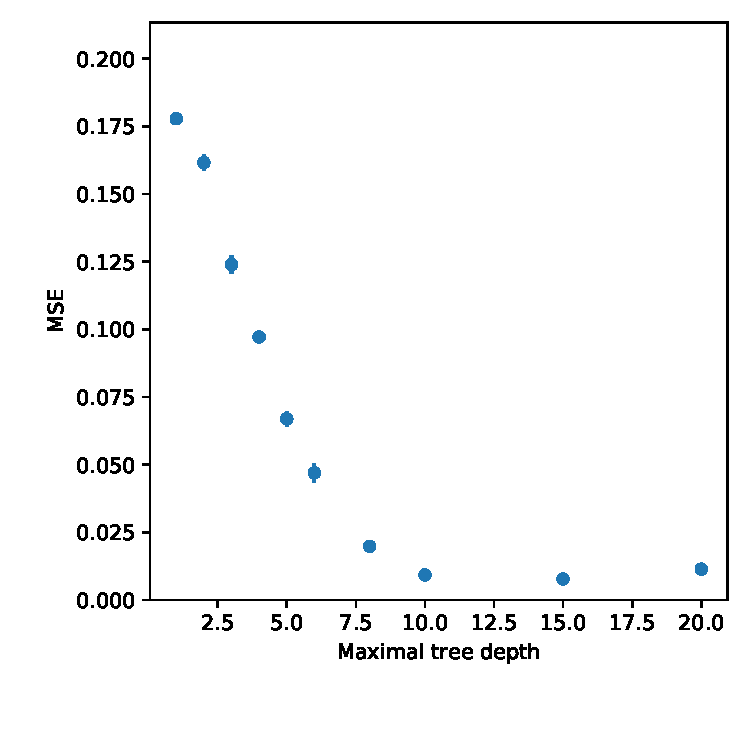
\includegraphics[height=0.45\textwidth]{figures/appendix/pointwise_tuning_2d/mse_rf_max_depths_alt.pdf}%
  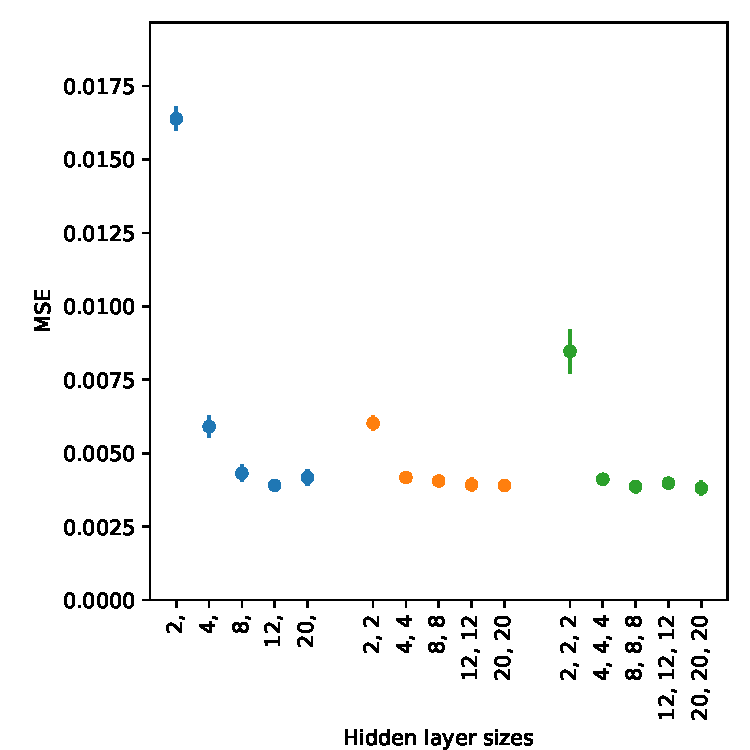
\includegraphics[width=0.45\textwidth]{figures/appendix/pointwise_tuning_2d/mse_mlp_hidden_layer_sizes_alt.pdf}%
  \caption{carl performance on the validation hypotheses for different
    hyperparameters.  We show the mean squred error of the estimated
    log likelihood ratio between two validation benchmark points for
    the 2D case. Each data point shows the mean of five calculations,
    the error bars are $95\%$ confidence intervals.}
  \label{fig:pointwise_validation_2d_tuning}
\end{figure}

All in all, we find that the neural net performs very well without
further fine-tuning, \ie that the same settings optimised on the
comparison of $\boldtheta_0$ versus $\boldtheta_1$ also work well for
$\boldtheta_0'$ versus $\boldtheta_1'$. The random forest, on the
other hand, is not so flexible. The two different hypothesis
comparisons require different choices of the maximal depth of the
trees, and what works best for one choice of parameter points leads to
a poor performance for a different choice. 



%%%%%%%%%%%%%%%%%%%%%%%%%%%%%%%%%%%%%%%%%%%%%%%%%%%%%%%%%%%%
\subsection{Likelihood contours}
%%%%%%%%%%%%%%%%%%%%%%%%%%%%%%%%%%%%%%%%%%%%%%%%%%%%%%%%%%%%

After optimizing our classifier setup on the distinction between two
distinct hypotheses, and validating the results on another two
hypotheses, we now turn towards the more relevant problem of
estimating $\boldtheta$ based on some measurements. We generate
25\,000 toy events sampled from the probability distribution for the
SM,
%
\begin{equation}
  \boldtheta_{\text{observed}} = \twovec 0 0 \,.
\end{equation} 
%
For 100 points randomly sampled in $\boldtheta \in [-0.9,0.9]^2$, we
calculate the true expected likelihood ratio to
%
\begin{equation}
  \boldtheta_{1} = \twovec {-0.23} {0.30}
\end{equation}
%
as well as the corresponding \toolfont{carl} estimate. Finally, we
interpolate between these points with a Gaussian Process with Mat\'ern
kernel with $\nu = 0.5$.

Following the results of the previous sections, for the
two-dimensional feature space we use a neural network with two hidden
layers of 8 neurons each, a $\tanh$ activation function, and a
regulator $\alpha = 0.001$. The training samples consist of 200\,000
unweighted samples each, and the $\toolfont{carl}$ default for the
fixed-size binning of the calibration histograms is used.

\begin{figure}
  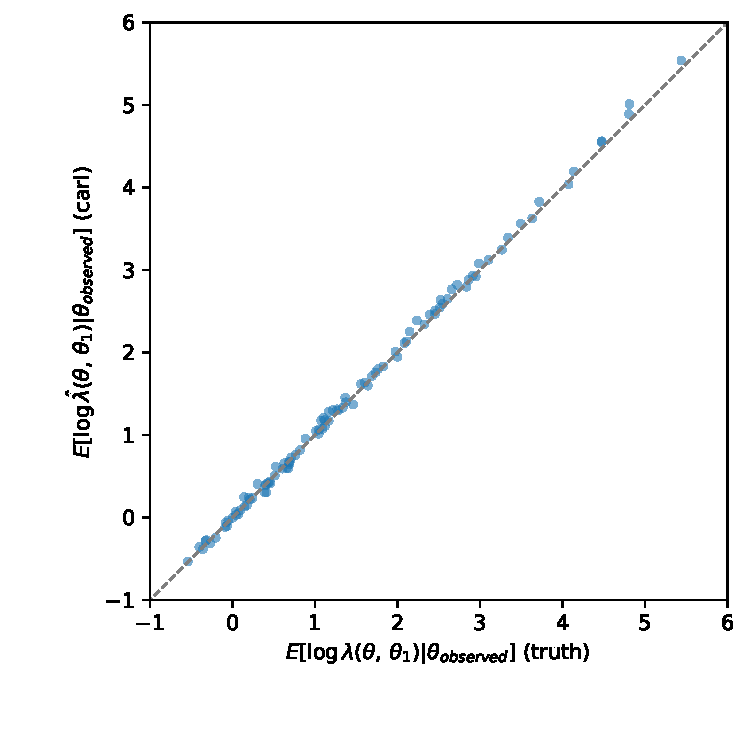
\includegraphics[height=0.45\textwidth]{figures/appendix/pointwise_inference/llr_truth_vs_carl_2d.pdf}%
  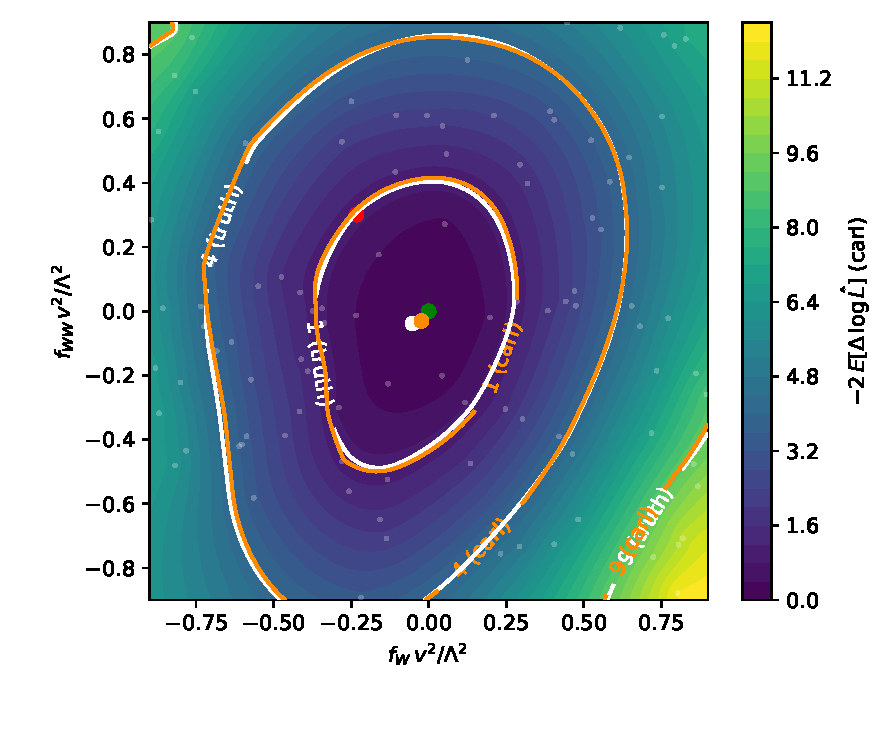
\includegraphics[height=0.45\textwidth]{figures/appendix/pointwise_inference/llr_gp_carl_2d.pdf}%
  \caption{Inference from truth likelihood ratio and \toolfont{carl}'s
    estimate for the 2D case. Left: scatter plot showing the
    difference between the exact expected likelihood ratio for 100
    randomly sampled points and $\boldtheta_1$ and \toolfont{carl}'s
    estimate. Right: true (white) and approximate (orange) likelihood
    contours, using a Gaussian Process for interpolation. The white
    and orange dots show the exact and approximate maximum-likelihood
    estimators. The green and red dots show
    $\boldtheta_{\text{observed}}$ and $\boldtheta_1$,
    respectively. Finally, the small grey dots show the sampled
    parameter points at which the likelihood ratio was evaluated.}
  \label{fig:pointwise_inference_2d}
\end{figure}

In \autoref{fig:pointwise_inference_2d} we show the results for the
two-dimensional feature space. The approximate likelihood map agrees
impressively well with the exact one. 










%%%%%%%%%%%%%%%%%%%%%%%%%%%%%%%%%%%%%%%%%%%%%%%%%%%%%%%%%%%%
\clearpage
\section{Detailed tuning of the point-by-point algorithms}
\label{sec:pointwise_tuning}
%%%%%%%%%%%%%%%%%%%%%%%%%%%%%%%%%%%%%%%%%%%%%%%%%%%%%%%%%%%%

One class of algorithms simplifies the inference problem by estimating
the likelihood ratio $r(\boldx ; \boldtheta_0, \boldtheta_1)$ for
different pairs $(\boldtheta_0, \boldtheta_1)$ separately. We analyse
two approaches: calibrated classification (\toolfont{carl}), and
regression on the likelihood ratio.



%%%%%%%%%%%%%%%%%%%%%%%%%%%%%%%%%%%%%%%%%%%%%%%%%%%%%%%%%%%%
\subsection{Calibrated classifiers}
%%%%%%%%%%%%%%%%%%%%%%%%%%%%%%%%%%%%%%%%%%%%%%%%%%%%%%%%%%%%

%%%%%%%%%%%%%%%%%%%%%%%%%%%%%%%%%%%%%%%%%%%%%%%%%%%%%%%%%%%%
\subsubsection{Benchmark hypothesis test}
%%%%%%%%%%%%%%%%%%%%%%%%%%%%%%%%%%%%%%%%%%%%%%%%%%%%%%%%%%%%

For two benchmark parameter points
%
\begin{equation}
  \boldtheta_0 = \twovec{-0.2} {-0.2} \,, \quad
  \boldtheta_1 = \twovec{0.2} {0.2}
\end{equation}
%
we first analyse how well \toolfont{carl} can estimate the likelihood ratio
%
\begin{equation}
  r(\boldx) = \frac {p(\boldx | \boldtheta_0)}  {p(\boldx | \boldtheta_1)}
\end{equation}
%
depending on the classifier, its hyperparameters, and a number of
different settings. 

\begin{figure}
  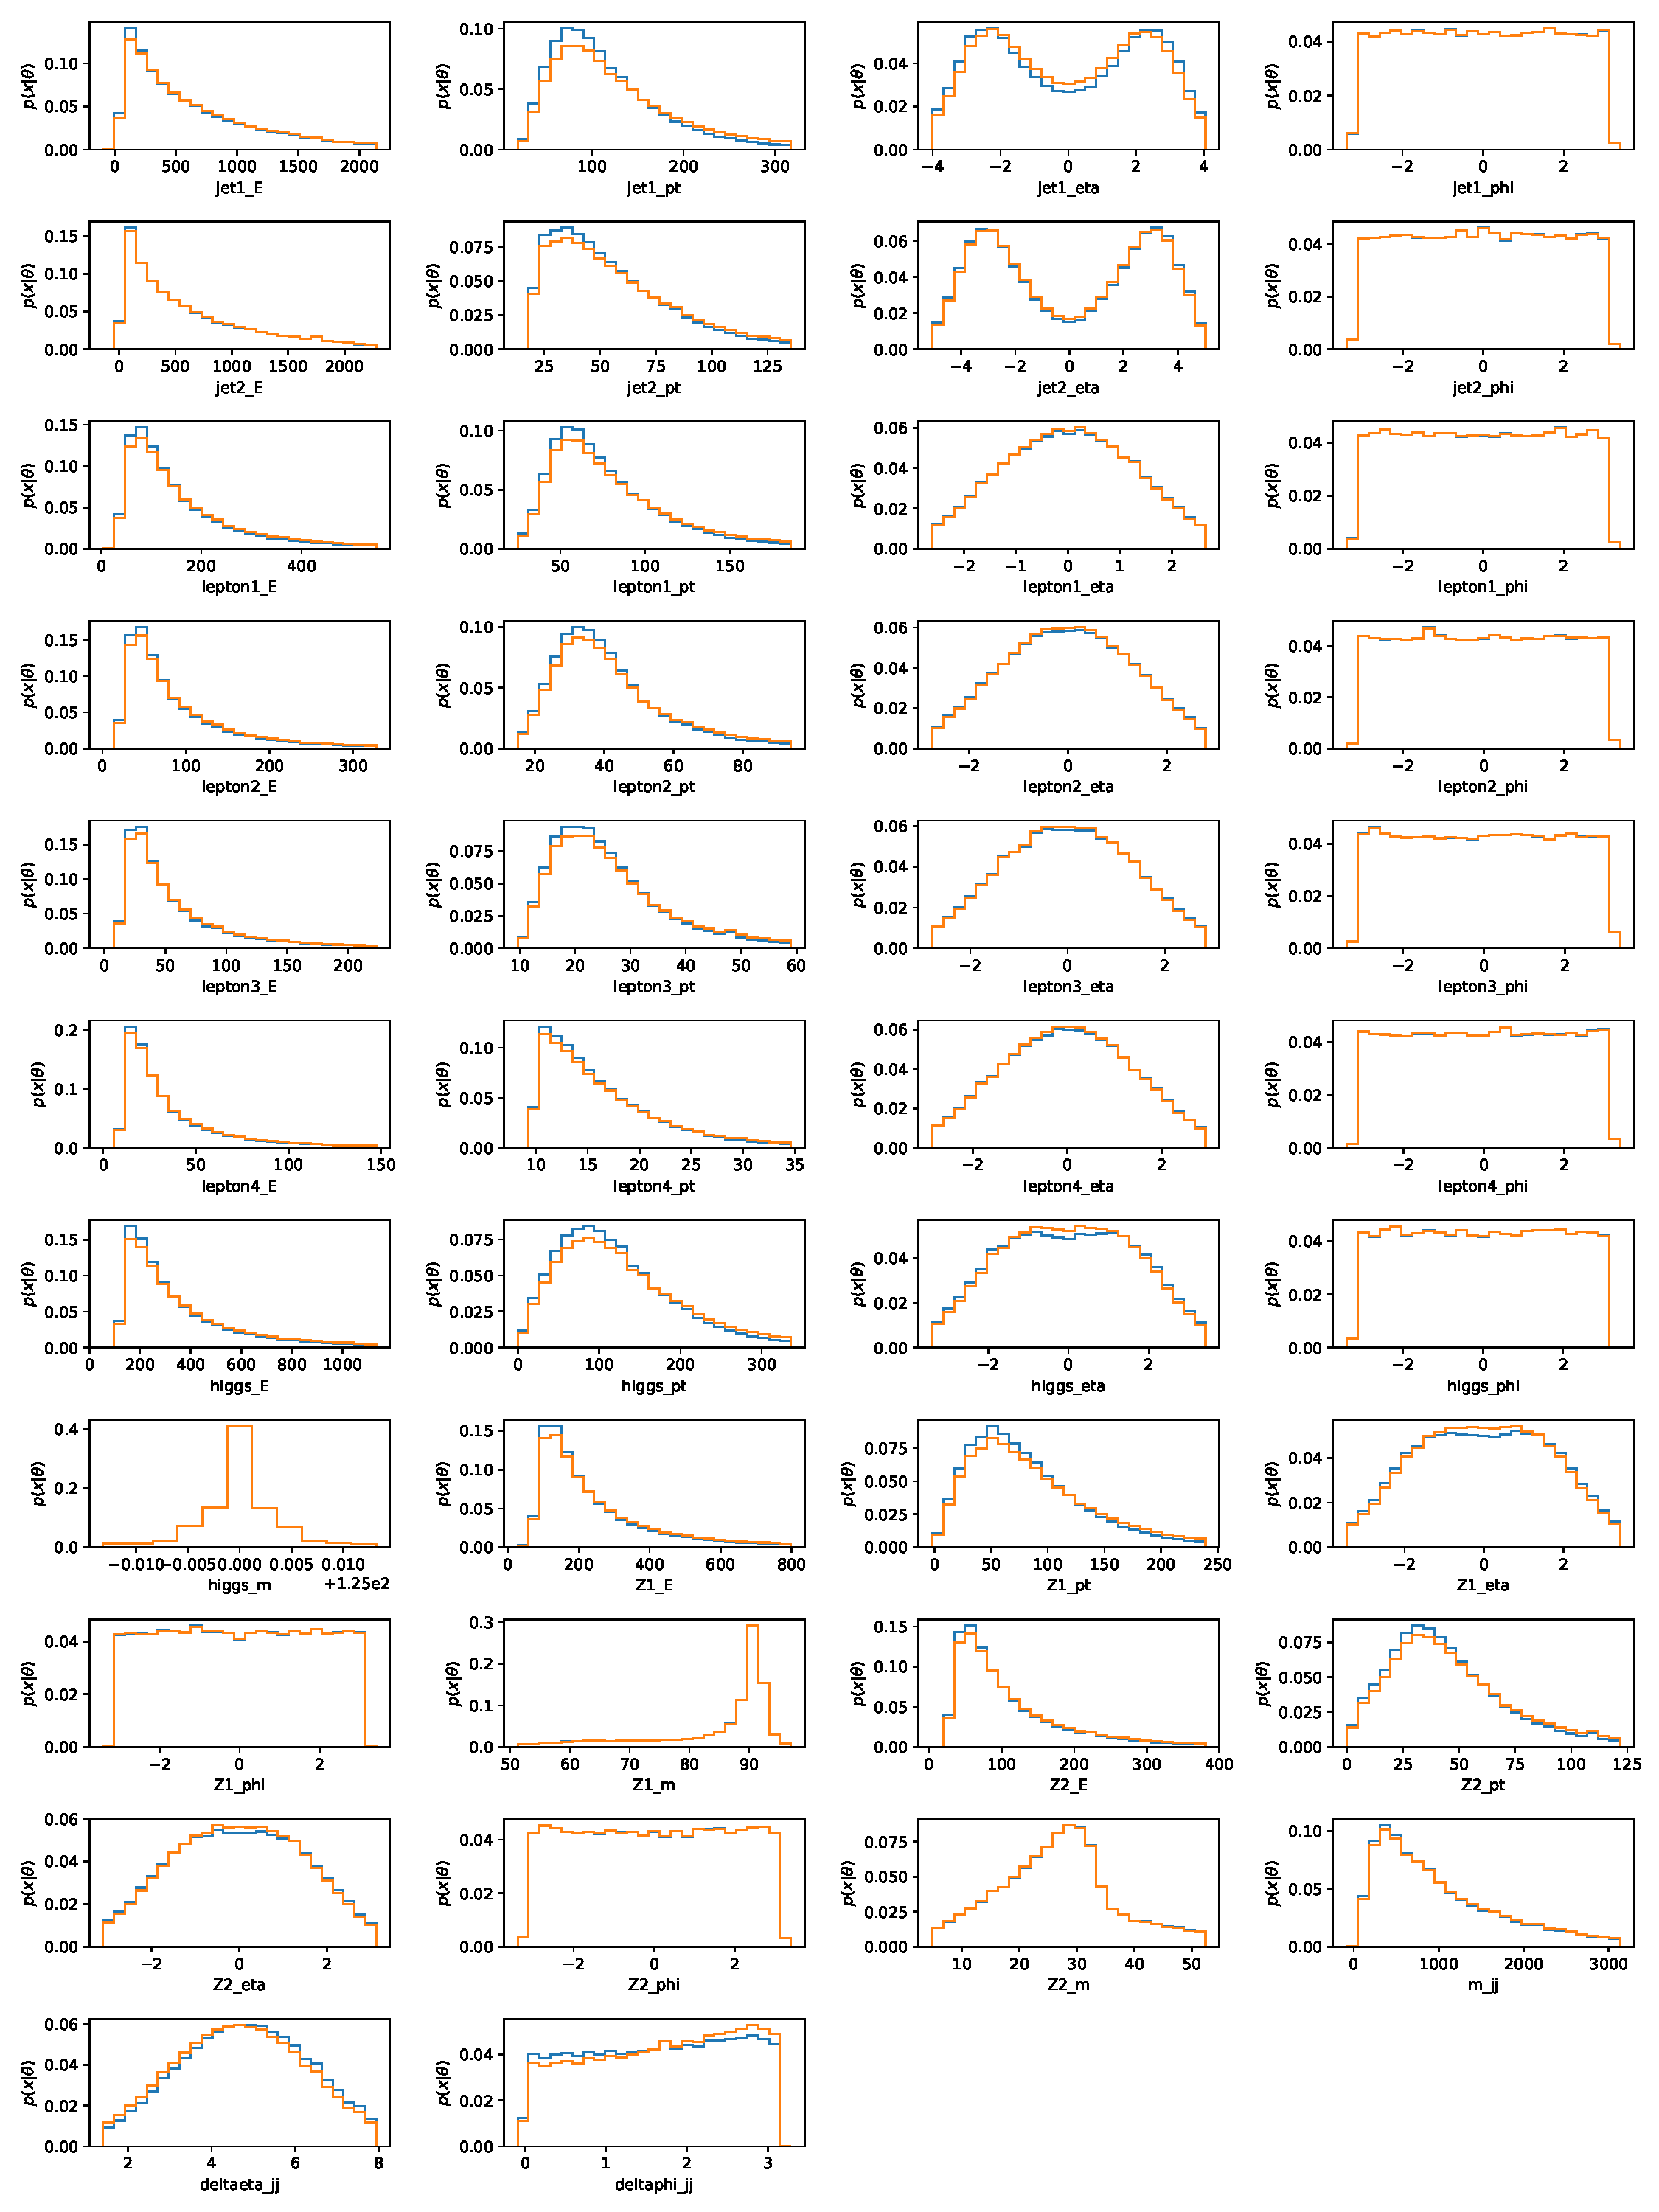
\includegraphics[width=\textwidth]{figures/appendix/pointwise_tuning_full/p_over_x.pdf}
  \caption{Distributions of all kinematic observables for $\boldtheta_0$ (blue) and $\boldtheta_1$ (orange).}
  \label{fig:pointwise_tuning_p_over_x}
\end{figure}

In \autoref{fig:pointwise_tuning_p_over_x} we show the distributions
of all 42 considered kinematic variables for these two parameter
points.

For each of the four feature sets outlined above (2D, medium set, full
kinematics, full kinematics plus derived variables), we tune the
parameters in two steps. First, we perform a randomized scan over
the hyperparameters, maximizing the classification power between event
samples sampled from $p(\boldx | \boldtheta_0)$ and
$p(\boldx | \boldtheta_1)$. In a second step we finetune these
parameters on the mean squared error between the \toolfont{carl}
estimate $\log \hat{r}(\boldx)$ and the true value $\log r(\boldx)$.

The first classifier we consider is a \emph{random forest}, more
precisely extremely randomized trees, in the
\toolfont{sklearn.ensemble.ExtraTreesClassifier} implementation. The
following parameters are tuned:
%
\begin{itemize}
  \item \toolfont{n\_estimators}, the number of trees in the forest;
  \item \toolfont{max\_features}, the number of features considered in
    the search for the best split;
  \item \toolfont{max\_depth}, the maximum depth of the trees;
  \item \toolfont{min\_samples\_split}, the minimum fraction of events
    at a node required for a split; and
  \item \toolfont{min\_samples\_leaf}, the minimum fraction of events
    in a leaf.
\end{itemize}

A \emph{multi-layer perceptron} implemented as a
\toolfont{sklearn.neural\_network.MLPClassifier} is our second
classifier. We optimize the following parameters:
%
\begin{itemize}
  \item \toolfont{hidden\_layer\_sizes}, describing the number of hidden
  layers and the number of neurons in each layer;
  \item \toolfont{activation}, the activation function; and
  \item \toolfont{alpha}, an $L^2$ penalty term.
\end{itemize}

For both classifiers, the kinematic features are first rescaled to a
normal distribution with a
\toolfont{sklearn.preprocessing.StandardScaler}.



%%%%%%%%%%%%%%%%%%%%%%%%%%%%%%%%%%%%%%%%%%%%%%%%%%%%%%%%%%%%
\subsubsection*{Estimators for the medium feature set}
%%%%%%%%%%%%%%%%%%%%%%%%%%%%%%%%%%%%%%%%%%%%%%%%%%%%%%%%%%%%

\begin{figure}
  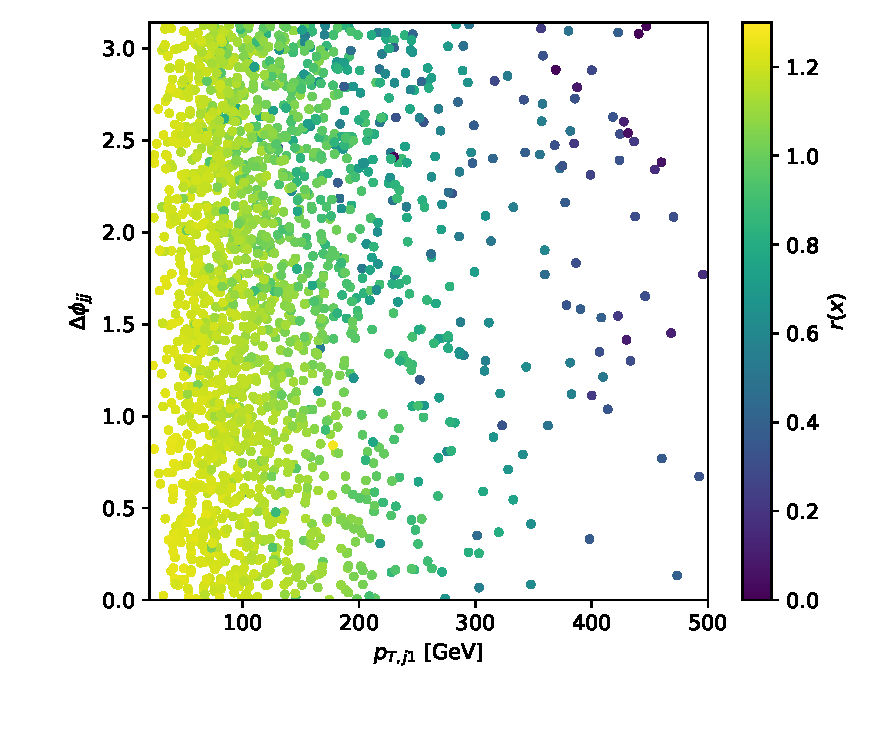
\includegraphics[height=0.45\textwidth]{figures/appendix/pointwise_tuning_full/r_over_x_2d.pdf}
  \caption{Truth likelihood ratio $r(\boldx)$ as defined in
    \autoref{eq:pointwise_tuning_r} for the fully differential
    kinematics as a function of two particular observables.}
  \label{fig:pointwise_tuning_full_r_x}
\end{figure}

We now try to see if we can estimate the fully differential likelihood
ratio equally well. This is a much more difficult problem:
\autoref{fig:pointwise_tuning_full_r_x} shows a scatter plot of the
truth likelihood ratio between the two points defined in
\autoref{eq:pointwise_tuning_benchmarks} over the jet $p_T$ and
$\Delta \phi_{jj}$, showing sizable fluctuations between close points
due to the other directions in phase space. First we train
$\toolfont{carl}$ on the medium set of 15 observables defined in
\autoref{sec:features}.

\begin{table}
\small
\begin{tabular}{ll r rrrr }
  \toprule 
  & Parameter & Range & Random & Bayes 1 & Bayes 2 & Benchmark \\
  \midrule
  RF & \toolfont{n\_estimators} & $50 \dots 200$ & $100$ &&& $100$ \\
  & \toolfont{max\_features} & $1 \dots 24$ & $6$ &&& $6$ \\
  & \toolfont{max\_depth} & $1 \dots 20, \infty$ & $12$ &&& $12$ \\
  & \toolfont{min\_samples\_split} & $0 \dots 1$ & $0$ &&& $0$ \\
  & \toolfont{min\_samples\_leaf} & $0 \dots 0.5$ & $0$ &&& $0$ \\
  \midrule
  NN & number of hidden layers & $1\dots 5$ & $2$ & $1$ & $1$ & $2$\\
  & neurons at each layer & $2\dots 100$ per layer & $(8,8)$ & $(5)$ & $(5)$ & $(8,8)$\\
  & activation function & $\tanh, \relu, \logistic$ & $\logistic$ & $\logistic$ & $\logistic$ & $\logistic$ \\
  & $\alpha$ & $0\dots 100$ & $0$ & $10^{-9}$ & $0$ & $0$\\
  & initial learning rate & $0.0001 \dots 0.01$ & & $0.01$ & $0.0067$ & $0.001$ \\
  \bottomrule
\end{tabular}
\caption{Hyperparameter scan on the classification problem between
  $\boldtheta_0$ and $\boldtheta_1$ using the medium feature set as input. For
  each parameter of the random forrest (RF) and the neural network (NN)
  we show the considered range and the best settings as determined by a randomized
  search CV, a Bayesian optimization procedure geared towards exploitation, and a Bayesian optimization procedure
  geared towards exploration. The final column shows our baseline parameters for the next step of the
  optimization procedure.}
 \label{tbl:pointwise_tuning_smart_parameters}
\end{table}

We first tune hyperparameters with a randomized scan on the
classification problem between unweighted event samples drawn from
$p(\boldx | \boldtheta_0)$ and $p(\boldx | \boldtheta_1)$. Using
\toolfont{sklearn.model\_selection.RandomizedSearchCV}, we optimize on
the ROC AUC. We give the optimal parameters in
\autoref{tbl:pointwise_tuning_full_parameters}. The optimal random
forests are now quite a bit deeper than in the 2d case.

\begin{figure}
  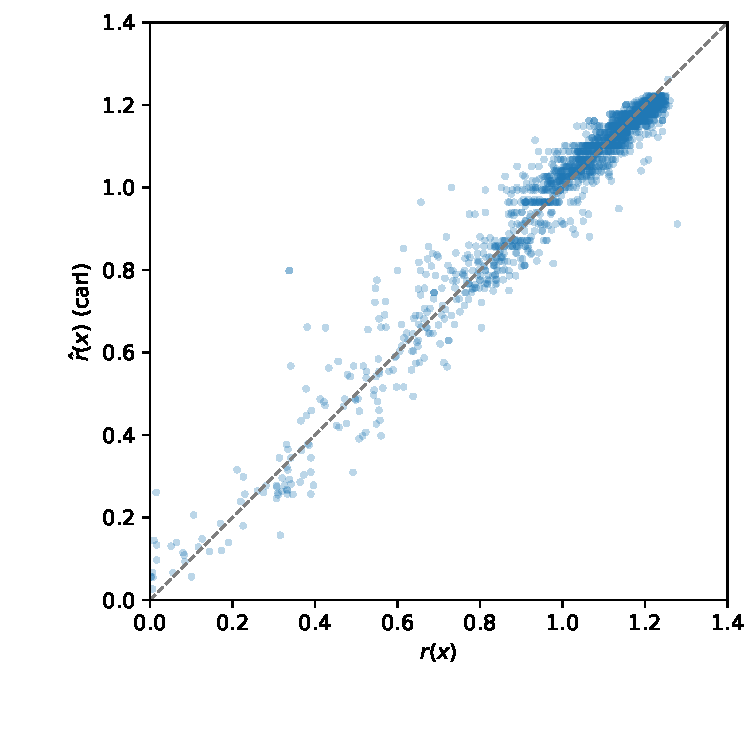
\includegraphics[height=0.45\textwidth]{figures/appendix/pointwise_tuning_full/rhat_vs_r_smart_rf.pdf}%
  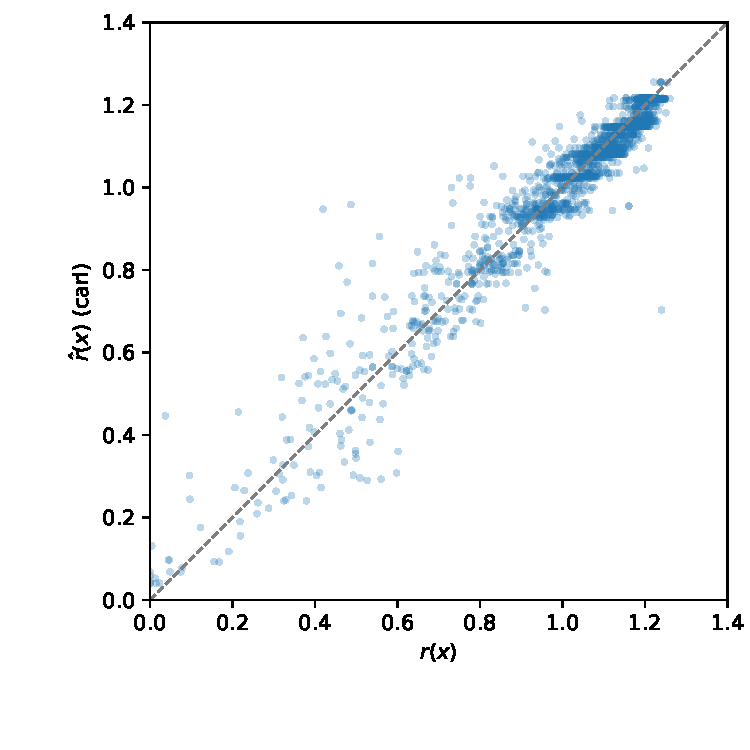
\includegraphics[height=0.45\textwidth]{figures/appendix/pointwise_tuning_full/rhat_vs_r_smart_mlp.pdf}%
  \caption{Likelihood ratio estimation with the tuned classifiers
    (left: random forest, right: neural network) using the medium feature set as
    input. We show a scatter plot between the true $r(\boldx)$ and the
    estimate $\hat{r}(\boldx)$.}
  \label{fig:pointwise_tuning_smart_performance}
\end{figure}

\begin{figure}
  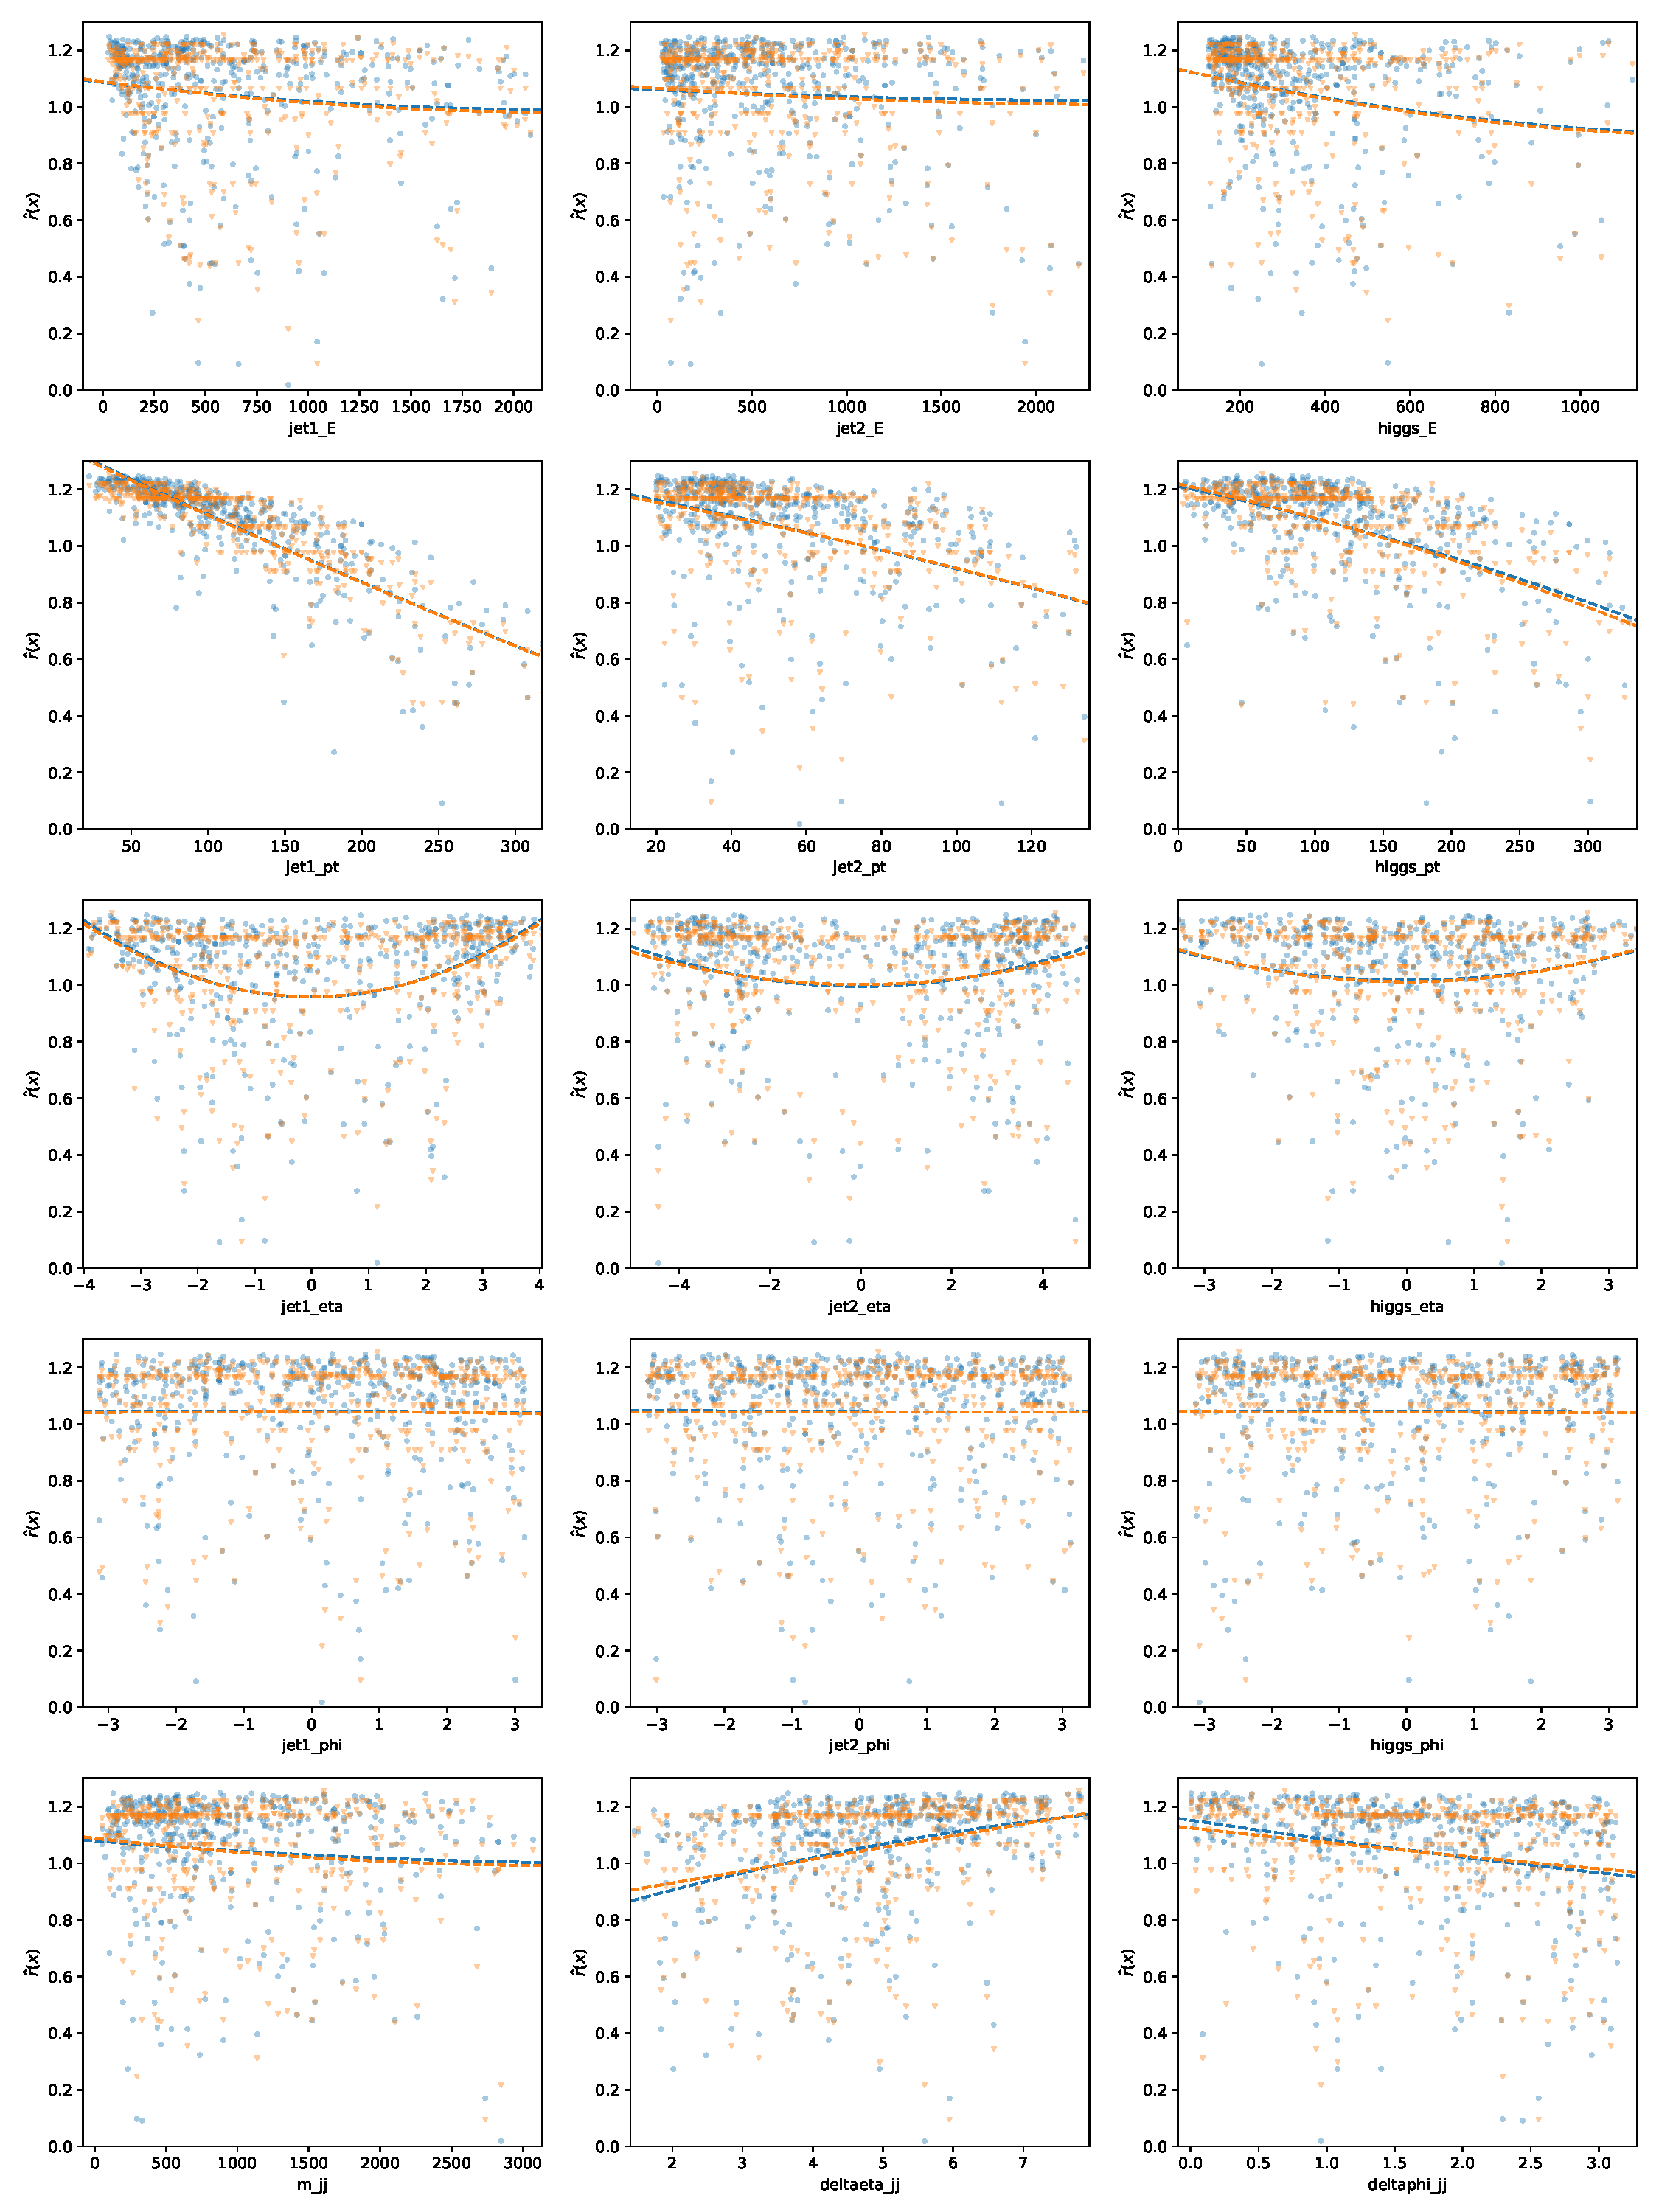
\includegraphics[width=\textwidth]{figures/appendix/pointwise_tuning_full/rhat_vs_x_smart_rf.pdf}
  \caption{Correlation of $r(\boldx)$ (blue) and $\toolfont{carl}$
    estimate $\hat{r}(\boldx)$ (orange) with various kinematic
    observables. As classifier we use the tuned random forest with the
    medium feature set as input. To guide the eye we also show fitted
    second-order polynomials.}
  \label{fig:pointwise_tuning_smart_rf_rhat_vs_x}
\end{figure}

In \autoref{fig:pointwise_tuning_smart_performance} we show how well
\toolfont{carl} can estimate the true likelihood ratio $r(\boldx)$
with the tuned classifiers given in the right column of
\autoref{tbl:pointwise_tuning_smart_parameters}. The performance is
much worse than in the 2d
case. \autoref{fig:pointwise_tuning_smart_rf_rhat_vs_x} shows a
scatter plot of the kinematic observables versus the exact ratio
$r(\boldx)$ and the estimate $\hat{r}(\boldx)$.

Next, we vary all parameters one by one and see how this affects the
mean squared error of $\log \hat{r}(\boldx)$. The results are shown in
Figures~\ref{fig:pointwise_tuning_smart_rf_tuning}.
and \ref{fig:pointwise_tuning_smart_mlp_tuning}.

\begin{figure}
  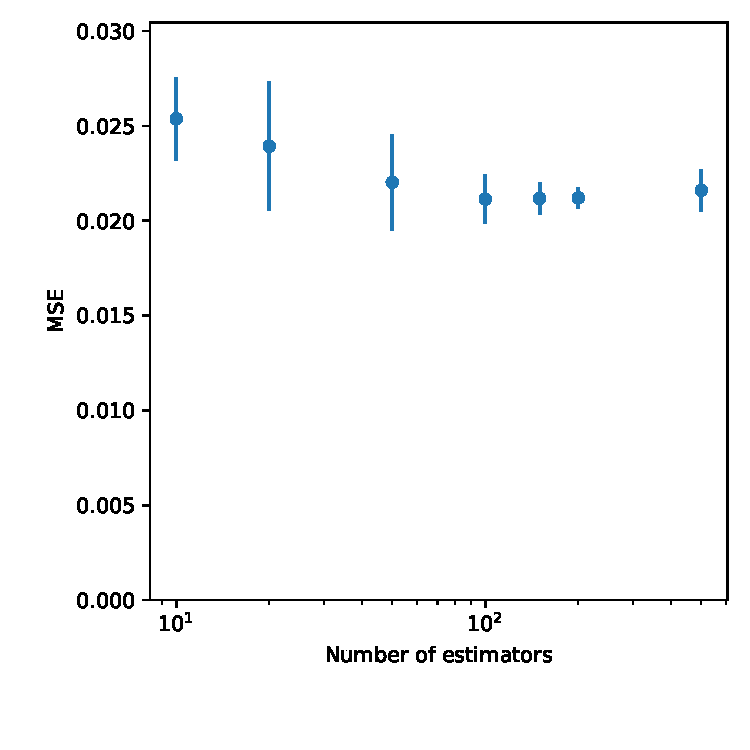
\includegraphics[width=0.45\textwidth]{figures/appendix/pointwise_tuning_full/mse_smart_rf_n_estimators.pdf}%
  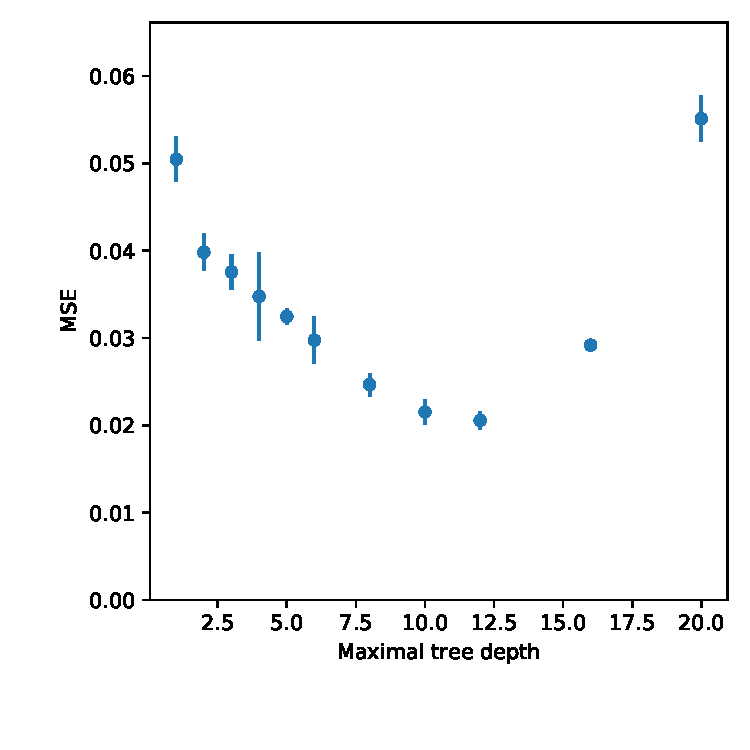
\includegraphics[height=0.45\textwidth]{figures/appendix/pointwise_tuning_full/mse_smart_rf_max_depths.pdf}\\%
  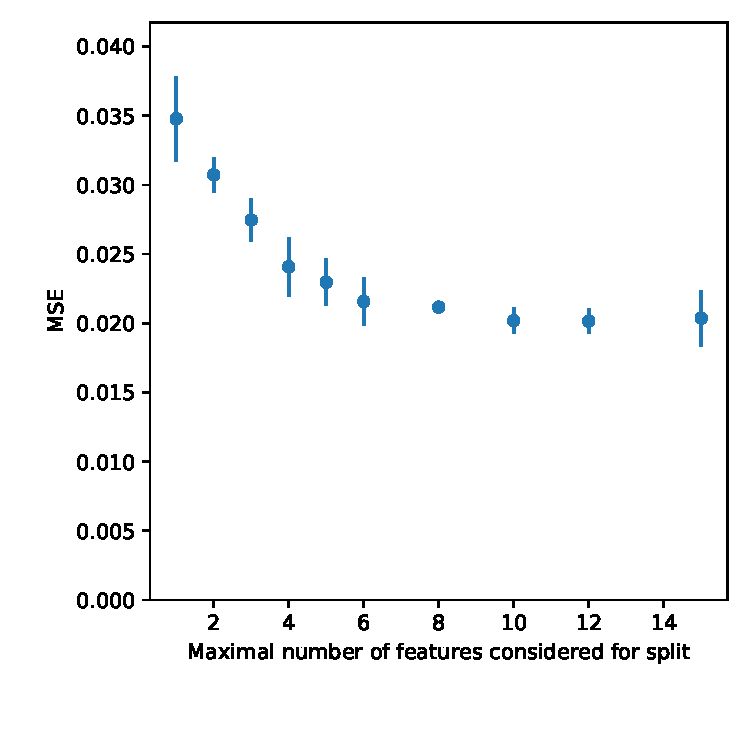
\includegraphics[height=0.45\textwidth]{figures/appendix/pointwise_tuning_full/mse_smart_rf_max_features.pdf}%
  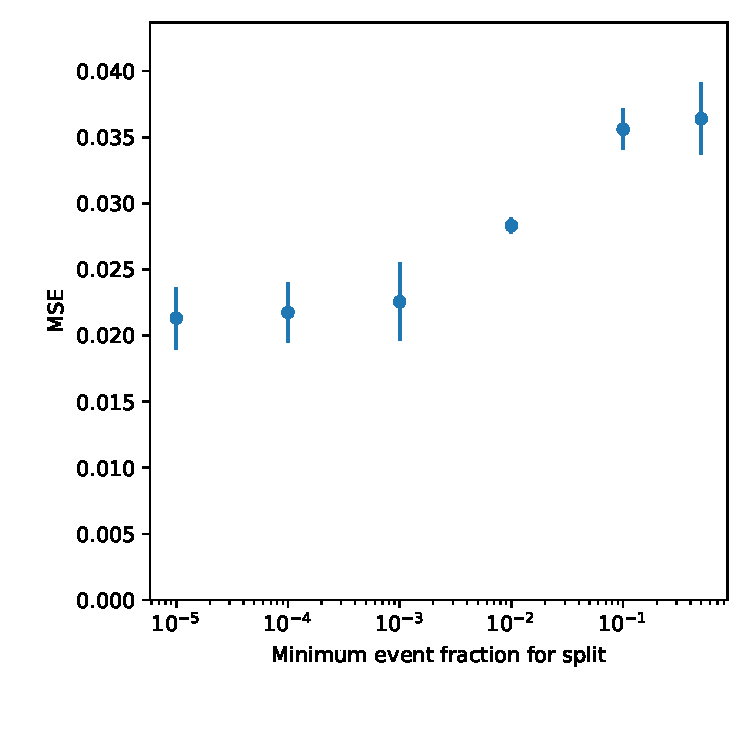
\includegraphics[height=0.45\textwidth]{figures/appendix/pointwise_tuning_full/mse_smart_rf_min_samples_splits.pdf}%
  \caption{carl performance as a function of the random forest
    hyperparameters. We show the mean squred error of the estimated
    log likelihood ratio between two benchmark points using the medium
    feature set as input. Each data point shows the mean of three
    calculations, the error bars are $95\%$ confidence intervals.}
  \label{fig:pointwise_tuning_smart_rf_tuning}
\end{figure}

\begin{figure}
  \includegraphics[width=0.45\textwidth]{figures/appendix/pointwise_tuning_full/mse_smart_mlp_hidden_layer_sizes.pdf}%
  \includegraphics[height=0.45\textwidth]{figures/appendix/pointwise_tuning_full/mse_smart_mlp_activation.pdf}\\%
  \includegraphics[height=0.45\textwidth]{figures/appendix/pointwise_tuning_full/mse_smart_mlp_alpha.pdf}%
  \caption{carl performance as a function of the neural network
  hyperparameters. Mean squred error of the estimated log likelihood
  ratio between two benchmark points using the medium feature set as
  input. Each data point shows the mean of three calculations, the
  error bars are $95\%$ confidence intervals.}
  \label{fig:pointwise_tuning_smart_mlp_tuning}
\end{figure}

For the random forest, the results of the hyperparameter scan lead to
a good performance, and there is no obvious reason to change any of
the settings in the right column of
\autoref{tbl:pointwise_tuning_smart_parameters}. For the neural
network, we define a final setup with a $\relu$ activation function
instead of the logistic one, with all other settings in the right
column of \autoref{tbl:pointwise_tuning_smart_parameters} unchanged.

% \begin{figure}
%   \includegraphics[width=0.45\textwidth]{figures/appendix/pointwise_tuning_full/mse_smart_training_sample_size.pdf}%
%   \caption{carl performance as a function of the training sample
%   size.  We show the mean squred error of the estimated log
%   likelihood ratio between two benchmark points using the medium
%   feature set as input. Each data point shows the mean of three
%   calculations, the error bars are $95\%$ confidence intervals.}
%   \label{fig:pointwise_tuning_smart_carl_tuning}
% \end{figure}

% \autoref{fig:pointwise_tuning_smart_carl_tuning} shows the effect of
% the size of the training samples.  Again, we choose 200\,000 events
% per sample as a compromise between computation time and performance. 




%%%%%%%%%%%%%%%%%%%%%%%%%%%%%%%%%%%%%%%%%%%%%%%%%%%%%%%%%%%%
\subsubsection*{Estimators for the full feature set}
%%%%%%%%%%%%%%%%%%%%%%%%%%%%%%%%%%%%%%%%%%%%%%%%%%%%%%%%%%%%

Now we use the full kinematics including the Higgs decay patterns,
parametrized by the 24 energies, transverse momenta, and angles given
in configuration 2 in
\autoref{sec:features}.

\begin{table}
\small
\begin{tabular}{ll r rrrr }
  \toprule 
  & Parameter & Range & Random & Bayes 1 & Bayes 2 & Benchmark \\
  \midrule
  RF & \toolfont{n\_estimators} & $50 \dots 200$ & $200$ &&& $200$ \\
  & \toolfont{max\_features} & $1 \dots 24$ & $20$ &&& $20$ \\
  & \toolfont{max\_depth} & $1 \dots 20, \infty$ & $12$ &&& $12$ \\
  & \toolfont{min\_samples\_split} & $0 \dots 1$ & $0.001$ &&& $0.001$ \\
  & \toolfont{min\_samples\_leaf} & $0 \dots 0.5$ & $0$ &&& $0$ \\
  \midrule
  NN & number of hidden layers & $1\dots 5$ & $2$ & $2$ & $2$ & $2$\\
  & neurons at each layer & $2\dots 100$ per layer & $(4,12)$ & $(50,50)$ & $(50,20)$ & $(4,12)$\\
  & activation function & $\tanh, \relu, \logistic$ & $\logistic$ & $\logistic$ & $\logistic$ & $\logistic$ \\
  & $\alpha$ & $0\dots 100$ & $0$ & $0$ & $10^{-9}$ & $0$\\
  & initial learning rate & $0.0001 \dots 0.01$ & & $0.0013$ & $0.0018$ & $0.001$ \\
  \bottomrule
\end{tabular}
\caption{Hyperparameter scan on the classification problem between
  $\boldtheta_0$ and $\boldtheta_1$ using the full feature set as input. For
  each parameter of the random forrest (RF) and the neural network (NN)
  we show the considered range and the best settings as determined by a randomized
  search CV, a Bayesian optimization procedure geared towards exploitation, and a Bayesian optimization procedure
  geared towards exploration. The final column shows our baseline parameters for the next step of the
  optimization procedure.}
 \label{tbl:pointwise_tuning_full_parameters}
\end{table}

We first tune hyperparameters with a randomized scan on the
classification problem between unweighted event samples drawn from
$p(\boldx | \boldtheta_0)$ and $p(\boldx | \boldtheta_1)$. Using
\toolfont{sklearn.model\_selection.RandomizedSearchCV}, we optimize on
the ROC AUC. We give the optimal parameters in
\autoref{tbl:pointwise_tuning_full_parameters}. The optimal random
forests are now quite a bit deeper than in the 2d case. For the neural
networks we find a surprising preference for small hidden layers, and
logistic activation functions are now preferred.

\begin{figure}
  \includegraphics[height=0.45\textwidth]{figures/appendix/pointwise_tuning_full/rhat_vs_r_full_rf.pdf}%
  \includegraphics[height=0.45\textwidth]{figures/appendix/pointwise_tuning_full/rhat_vs_r_full_mlp.pdf}%
  \caption{Likelihood ratio estimation with the tuned classifiers
    (left: random forest, right: neural network) using the full
    feature set as input. We show a scatter plot between the true
    $r(\boldx)$ and the estimate $\hat{r}(\boldx)$}.
  \label{fig:pointwise_tuning_full_rf_performance}
\end{figure}

In \autoref{fig:pointwise_tuning_full_rf_performance} we show how well
\toolfont{carl} can estimate the true likelihood ratio $r(\boldx)$
with the tuned classifiers given in the right column of
\autoref{tbl:pointwise_tuning_full_parameters}. The performance is
much worse than in the 2d case.

Next, we vary all parameters one by one and see how this affects the
mean squared error of $\log \hat{r}(\boldx)$. The results are shown in
Figures~\ref{fig:pointwise_tuning_full_rf_tuning} to
\ref{fig:pointwise_tuning_full_carl_tuning}. For the random forest, we
again find that the parameters tuned on the classification problem
already lead to a good performance for the estimation of
$r(\boldx)$. For the neural network, switching to the $\relu$
activation function improves the estimation, so we use it in our final
setup.

\begin{figure}
  \includegraphics[width=0.45\textwidth]{figures/appendix/pointwise_tuning_full/mse_full_rf_n_estimators.pdf}%
  \includegraphics[height=0.45\textwidth]{figures/appendix/pointwise_tuning_full/mse_full_rf_max_depths.pdf}\\%
  \includegraphics[height=0.45\textwidth]{figures/appendix/pointwise_tuning_full/mse_full_rf_max_features.pdf}%
  \includegraphics[height=0.45\textwidth]{figures/appendix/pointwise_tuning_full/mse_full_rf_min_samples_splits.pdf}%
  \caption{carl performance as a function of the random forest
    hyperparameters. We show the mean squred error of the estimated
    log likelihood ratio between two benchmark points using the full
    feature set as input. Each data point shows the mean of three
    calculations, the error bars are $95\%$ confidence intervals.}
  \label{fig:pointwise_tuning_full_rf_tuning}
\end{figure}

\begin{figure}
  \includegraphics[width=0.45\textwidth]{figures/appendix/pointwise_tuning_full/mse_full_mlp_hidden_layer_sizes.pdf}%
  \includegraphics[height=0.45\textwidth]{figures/appendix/pointwise_tuning_full/mse_full_mlp_activation.pdf}\\%
  \includegraphics[height=0.45\textwidth]{figures/appendix/pointwise_tuning_full/mse_full_mlp_alpha.pdf}%
  \caption{carl performance as a function of the neural network
    hyperparameters. We show the mean squred error of the estimated
    log likelihood ratio between two benchmark points using the full
    feature set as input. Each data point shows the mean of three
    calculations, the error bars are $95\%$ confidence intervals.}
  \label{fig:pointwise_tuning_full_mlp_tuning}
\end{figure}

\begin{figure}
  \includegraphics[width=0.45\textwidth]{figures/appendix/pointwise_tuning_full/mse_full_training_sample_size.pdf}%
  \caption{carl performance as a function of the training sample size.
    We show the mean squred error of the estimated log likelihood
    ratio between two benchmark points using the full feature set as
    input. Each data point shows the mean of three calculations, the
    error bars are $95\%$ confidence intervals.}
  \label{fig:pointwise_tuning_full_carl_tuning}
\end{figure}

\autoref{fig:pointwise_tuning_full_carl_tuning} shows the effect of
the size of the training samples.  Again, we choose 200\,000 events
per sample as a compromise between computation time and performance.




%%%%%%%%%%%%%%%%%%%%%%%%%%%%%%%%%%%%%%%%%%%%%%%%%%%%%%%%%%%%
\subsubsection*{Estimators for the full plus derived feature set}
%%%%%%%%%%%%%%%%%%%%%%%%%%%%%%%%%%%%%%%%%%%%%%%%%%%%%%%%%%%%

Finally, we analyse whether the estimator is improved if we include an
additional 18 derived quantities, see \autoref{sec:features}. The
results of the hyperparameter scan are given in
\autoref{tbl:pointwise_tuning_full_parameters}.

\begin{table}
\small
\begin{tabular}{ll r rrrr }
  \toprule 
  & Parameter & Range & Random & Bayes 1 & Bayes 2 & Benchmark \\
  \midrule
  RF & \toolfont{n\_estimators} & $50 \dots 200$ & $200$ &&& $200$ \\
  & \toolfont{max\_features} & $1 \dots 42$ & $42$ &&& $42$ \\
  & \toolfont{max\_depth} & $1 \dots 20, \infty$ & $10$ &&& $10$ \\
  & \toolfont{min\_samples\_split} & $0 \dots 1$ & $0.001$ &&& $0.001$ \\
  & \toolfont{min\_samples\_leaf} & $0 \dots 0.5$ & $0$ &&& $0$ \\
  \midrule
  NN & number of hidden layers & $1\dots 5$ & $2$ & $2$ & $2$ & $2$\\
  & neurons at each layer & $2\dots 100$ per layer & $(4,12)$ & $(5,5)$ & $(100,100)$ & $(4,12)$\\
  & activation function & $\tanh, \relu, \logistic$ & $\logistic$ & $\logistic$ & $\logistic$ & $\logistic$ \\
  & $\alpha$ & $0\dots 100$ & $0$ & $10^{-8}$ & $0$ & $0$\\
  & initial learning rate & $0.0001 \dots 0.01$ & & $0.00022$ & $0.00064$ & $0.001$ \\
  \bottomrule
\end{tabular}
\caption{Hyperparameter scan on the classification problem between
  $\boldtheta_0$ and $\boldtheta_1$ using the full plus derived
  feature set as input. For
  each parameter of the random forrest (RF) and the neural network (NN)
  we show the considered range and the best settings as determined by a randomized
  search CV, a Bayesian optimization procedure geared towards exploitation, and a Bayesian optimization procedure
  geared towards exploration. The final column shows our baseline parameters for the next step of the
  optimization procedure.}
 \label{tbl:pointwise_tuning_derived_parameters}
\end{table}

In \autoref{fig:pointwise_tuning_derived_performance} we show how well
\toolfont{carl} can estimate the true likelihood ratio $r(\boldx)$
with the tuned classifiers given in the right column of
\autoref{tbl:pointwise_tuning_derived_parameters}. The performance is
slightly better than without the derived variables.

\begin{figure}
  \includegraphics[height=0.45\textwidth]{figures/appendix/pointwise_tuning_full/rhat_vs_r_derived_rf.pdf}%
  \includegraphics[height=0.45\textwidth]{figures/appendix/pointwise_tuning_full/rhat_vs_r_derived_mlp.pdf}%
  \caption{Likelihood ratio estimation with the tuned classifiers
    (left: random forest, right: neural network) using the full plus
    derived feature set as input. We show a scatter plot between the
    true $r(\boldx)$ and the estimate $\hat{r}(\boldx)$.}.
  \label{fig:pointwise_tuning_derived_performance}
\end{figure}

Again, we vary the parameters one by one and check if we can improve
the performance, see
Figures~\ref{fig:pointwise_tuning_derived_rf_tuning} to
\ref{fig:pointwise_tuning_derived_carl_tuning}. The results mirror
those in the previous section. The only improvement we can find is
switching to the $\relu$ activation function for the neural network in
our final setup, all other settings remain as in the right column of
\autoref{tbl:pointwise_tuning_derived_parameters}.

\begin{figure}
  \includegraphics[width=0.45\textwidth]{figures/appendix/pointwise_tuning_full/mse_derived_rf_n_estimators.pdf}%
  \includegraphics[height=0.45\textwidth]{figures/appendix/pointwise_tuning_full/mse_derived_rf_max_depths.pdf}\\%
  \includegraphics[height=0.45\textwidth]{figures/appendix/pointwise_tuning_full/mse_derived_rf_max_features.pdf}%
  \includegraphics[height=0.45\textwidth]{figures/appendix/pointwise_tuning_full/mse_derived_rf_min_samples_splits.pdf}%
  \caption{carl performance as a function of the random forest
    hyperparameters. We show the mean squred error of the estimated
    log likelihood ratio between two benchmark points using the full
    plus derived feature set as input. Each data point shows the mean
    of three calculations, the error bars are $95\%$ confidence
    intervals.}
  \label{fig:pointwise_tuning_derived_rf_tuning}
\end{figure}

\begin{figure}
  \includegraphics[width=0.45\textwidth]{figures/appendix/pointwise_tuning_full/mse_derived_mlp_hidden_layer_sizes.pdf}%
  \includegraphics[height=0.45\textwidth]{figures/appendix/pointwise_tuning_full/mse_derived_mlp_activation.pdf}\\%
  \includegraphics[height=0.45\textwidth]{figures/appendix/pointwise_tuning_full/mse_derived_mlp_alpha.pdf}%
  \caption{carl performance as a function of the neural network
    hyperparameters. We show the mean squred error of the estimated
    log likelihood ratio between two benchmark points using the full
    plus derived feature set as input. Each data point shows the mean
    of three calculations, the error bars are $95\%$ confidence
    intervals.}
  \label{fig:pointwise_tuning_derived_mlp_tuning}
\end{figure}

\begin{figure}
  \includegraphics[width=0.45\textwidth]{figures/appendix/pointwise_tuning_full/mse_derived_training_sample_size.pdf}%
  \caption{carl performance as a function of the training sample size.
    We show the mean squred error of the estimated log likelihood
    ratio between two benchmark points using the full plus derived
    feature set as input. Each data point shows the mean of three
    calculations, the error bars are $95\%$ confidence intervals.}
  \label{fig:pointwise_tuning_derived_carl_tuning}
\end{figure}




%%%%%%%%%%%%%%%%%%%%%%%%%%%%%%%%%%%%%%%%%%%%%%%%%%%%%%%%%%%%
\subsubsection*{Calibration}
%%%%%%%%%%%%%%%%%%%%%%%%%%%%%%%%%%%%%%%%%%%%%%%%%%%%%%%%%%%%

We now stick to a random forest trained on the medium feature set with
hyperparameters as given in the last column of
\autoref{tbl:pointwise_tuning_smart_parameters} and have a closer look
at \toolfont{carl}'s calibration procedure.

\begin{figure}
  \includegraphics[width=0.45\textwidth]{figures/appendix/pointwise_tuning_full/rhat_vs_r_smart_rf_uncalibrated.pdf}%
  \includegraphics[width=0.45\textwidth]{figures/appendix/pointwise_tuning_full/rhat_vs_r_smart_rf.pdf}%
  \caption{Likelihood ratio estimation with uncalibrated (left) vs
    calibrated (right) random forests. We show a scatter plot between
    the true $r(\boldx)$ and the estimate $\hat{r}(\boldx)$.}
  \label{fig:pointwise_tuning_smart_calibration}
\end{figure}

First, \autoref{fig:pointwise_tuning_smart_calibration} shows the
output of an uncalibrated classifier and compares it to the calibrated
classifier. Clearly, calibration improves the performance. 

\begin{figure}
  \includegraphics[width=0.45\textwidth]{figures/appendix/pointwise_tuning_full/mse_full_calibration_method.pdf}%
  \includegraphics[width=0.45\textwidth]{figures/appendix/pointwise_tuning_full/mse_full_cv_folds.pdf}\\%
  \includegraphics[width=0.45\textwidth]{figures/appendix/pointwise_tuning_full/mse_full_calibration_bins.pdf}%
  \includegraphics[width=0.45\textwidth]{figures/appendix/pointwise_tuning_full/mse_full_calibration_bins_variable.pdf}%
  \caption{Performance of \toolfont{carl} as a function of the
    calibration method and its parameters. Top left: different
    calibration algorithms. Top right: different cross-validation
    setups for the histogram validation. Bottom left: different number
    of bins for the histogram calibration. Bottom right: Same, also
    showing the results for variable bin widths. We show the mean
    squred error of the estimated log likelihood ratio between two
    benchmark points using the medium feature set as input. Each data
    point shows the mean of three calculations, the error bars are
    $95\%$ confidence intervals.}
  \label{fig:pointwise_tuning_smart_calibration_tuning}
\end{figure}

\autoref{fig:pointwise_tuning_smart_calibration_tuning} shows how the
performance of \toolfont{carl} depends on the calibration method and
its settings. The best results come from the simple histogram
calibration (with equidistant bin sizes) or an isotonic calibration.

\begin{figure}
  \includegraphics[width=0.45\textwidth]{figures/appendix/pointwise_tuning_full/s_raw_vs_cal_one_smart_rf.pdf}%
  \includegraphics[width=0.45\textwidth]{figures/appendix/pointwise_tuning_full/s_raw_vs_cal_average_smart_rf.pdf}\\%
  \includegraphics[width=0.45\textwidth]{figures/appendix/pointwise_tuning_full/average_s_raw_vs_rhat_smart_rf.pdf}%
  \caption{Details of the histogram calibration procedure. Top left:
    correlation between raw $s(\boldx)$ from one random forest and the
    corresponding calibrated values. Top right: correlation between
    average raw $s(\boldx)$ from all random forests in the
    cross-validator and the average calibrated $s(\boldx)$. Bottom:
    correlation between average raw $s(\boldx)$ from all random
    forests in the cross-validator and the final output
    $\hat{r}(\boldx)$.}
  \label{fig:pointwise_tuning_smart_calibration_histogram1}
\end{figure}

\begin{figure}
  \includegraphics[width=0.45\textwidth]{figures/appendix/pointwise_tuning_full/calibration_histos_one_smart_rf.pdf}%
  \includegraphics[width=0.45\textwidth]{figures/appendix/pointwise_tuning_full/s_histos_one_log_smart_rf.pdf}\\%
  \includegraphics[width=0.45\textwidth]{figures/appendix/pointwise_tuning_full/s_histos_average_smart_rf.pdf}%
  \includegraphics[width=0.45\textwidth]{figures/appendix/pointwise_tuning_full/s_histos_average_log_smart_rf.pdf}%
  \caption{Calibration histograms. Top left: actual calibration
    histogram for one random forest. Top right: distribution of the
    raw and calibrated values of $s(\boldx)$ for one random
    forest. Bottom left: distribution of the average raw and average
    calibrated values of $s(\boldx)$ for the ensemble of all random
    forests. Bottom right: same, but with a logarithmic $y$ axis.}
  \label{fig:pointwise_tuning_smart_calibration_histogram2}
\end{figure}

\begin{figure}
  \includegraphics[width=0.45\textwidth]{figures/appendix/pointwise_tuning_full/s_raw_vs_cal_one_smart_rf_isotonic.pdf}%
  \includegraphics[width=0.45\textwidth]{figures/appendix/pointwise_tuning_full/s_raw_vs_cal_average_smart_rf_isotonic.pdf}\\%
  \includegraphics[width=0.45\textwidth]{figures/appendix/pointwise_tuning_full/average_s_raw_vs_rhat_smart_rf_isotonic.pdf}%
  \caption{Details of the isotonic calibration procedure. Top left:
    correlation between raw $s(\boldx)$ from one random forest and the
    corresponding calibrated values. Top right: correlation between
    average raw $s(\boldx)$ from all random forests in the
    cross-validator and the average calibrated $s(\boldx)$. Bottom:
    correlation between average raw $s(\boldx)$ from all random
    forests in the cross-validator and the final output
    $\hat{r}(\boldx)$.}
  \label{fig:pointwise_tuning_smart_calibration_isotonic}
\end{figure}

In \autoref{fig:pointwise_tuning_smart_calibration_histogram1} and
\autoref{fig:pointwise_tuning_smart_calibration_histogram2} we
illuminate the relation between raw and calibrated $s(\boldx)$ for the
default histogram-based
calibration with fixed bin widths. \autoref{fig:pointwise_tuning_smart_calibration_isotonic}
does the same for isotonic calibration. Both calibration procedures
work as expected.

\begin{figure}
  \includegraphics[width=0.45\textwidth]{figures/appendix/pointwise_tuning_full/s_raw_vs_cal_one_smart_rf_var_binwidth.pdf}%
  \includegraphics[width=0.45\textwidth]{figures/appendix/pointwise_tuning_full/s_raw_vs_cal_average_smart_rf_var_binwidth.pdf}\\%
  \includegraphics[width=0.45\textwidth]{figures/appendix/pointwise_tuning_full/average_s_raw_vs_rhat_smart_rf_var_binwidth.pdf}%
  \caption{Details of the histogram calibration procedure with
    variable bin width, with different binnings for nominator and
    denominator. Top left: correlation between raw $s(\boldx)$ from
    one random forest and the corresponding calibrated values. Top
    right: correlation between average raw $s(\boldx)$ from all random
    forests in the cross-validator and the average calibrated
    $s(\boldx)$. Bottom: correlation between average raw $s(\boldx)$
    from all random forests in the cross-validator and the final
    output $\hat{r}(\boldx)$.}
  \label{fig:pointwise_tuning_smart_calibration_histogram_varwidth1}
\end{figure}

\begin{figure}
  \includegraphics[width=0.45\textwidth]{figures/appendix/pointwise_tuning_full/calibration_histos_one_smart_rf_var_binwidth.pdf}%
  \includegraphics[width=0.45\textwidth]{figures/appendix/pointwise_tuning_full/s_histos_one_log_smart_rf_var_binwidth.pdf}\\%
  \includegraphics[width=0.45\textwidth]{figures/appendix/pointwise_tuning_full/s_histos_average_smart_rf_var_binwidth.pdf}%
  \includegraphics[width=0.45\textwidth]{figures/appendix/pointwise_tuning_full/s_histos_average_log_smart_rf_var_binwidth.pdf}%
  \caption{Calibration histograms with variable bin width, with
    different binnings for nominator and denominator. Top left: actual
    calibration histogram for one random forest. Top right:
    distribution of the raw and calibrated values of $s(\boldx)$ for
    one random forest. Bottom left: distribution of the average raw
    and average calibrated values of $s(\boldx)$ for the ensemble of
    all random forests. Bottom right: same, but with a logarithmic $y$
    axis.}
  \label{fig:pointwise_tuning_smart_calibration_histogram_varwidth2}
\end{figure}

\begin{figure}
  \includegraphics[width=0.45\textwidth]{figures/appendix/pointwise_tuning_full/s_raw_vs_cal_one_smart_rf_var_binwidth_common.pdf}%
  \includegraphics[width=0.45\textwidth]{figures/appendix/pointwise_tuning_full/s_raw_vs_cal_average_smart_rf_var_binwidth_common.pdf}\\%
  \includegraphics[width=0.45\textwidth]{figures/appendix/pointwise_tuning_full/average_s_raw_vs_rhat_smart_rf_var_binwidth_common.pdf}%
  \caption{Details of the histogram calibration procedure with
    variable bin width, with common binning for nominator and
    denominator. Top left: correlation between raw $s(\boldx)$ from
    one random forest and the corresponding calibrated values. Top
    right: correlation between average raw $s(\boldx)$ from all random
    forests in the cross-validator and the average calibrated
    $s(\boldx)$. Bottom: correlation between average raw $s(\boldx)$
    from all random forests in the cross-validator and the final
    output $\hat{r}(\boldx)$.}
  \label{fig:pointwise_tuning_smart_calibration_histogram_varwidth3}
\end{figure}

\begin{figure}
  \includegraphics[width=0.45\textwidth]{figures/appendix/pointwise_tuning_full/calibration_histos_one_smart_rf_var_binwidth_common.pdf}%
  \includegraphics[width=0.45\textwidth]{figures/appendix/pointwise_tuning_full/s_histos_one_log_smart_rf_var_binwidth_common.pdf}\\%
  \includegraphics[width=0.45\textwidth]{figures/appendix/pointwise_tuning_full/s_histos_average_smart_rf_var_binwidth_common.pdf}%
  \includegraphics[width=0.45\textwidth]{figures/appendix/pointwise_tuning_full/s_histos_average_log_smart_rf_var_binwidth_common.pdf}%
  \caption{Calibration histograms with variable bin width, with common
    binning for nominator and denominator. Top left: actual
    calibration histogram for one random forest. Top right:
    distribution of the raw and calibrated values of $s(\boldx)$ for
    one random forest. Bottom left: distribution of the average raw
    and average calibrated values of $s(\boldx)$ for the ensemble of
    all random forests. Bottom right: same, but with a logarithmic $y$
    axis.}
  \label{fig:pointwise_tuning_smart_calibration_histogram_varwidth4}
\end{figure}

Figures~\ref{fig:pointwise_tuning_smart_calibration_histogram_varwidth1}
to \ref{fig:pointwise_tuning_smart_calibration_histogram_varwidth4}
show the same plots for the histogram calibration procedure with
variable bin width. Different bin boundaries for the nominator and
denominator histograms lead to problems (see the weird behaviour at
$s \gtrsim 0.6$). But even with a common binning, the variable-width
calibration setup performs worse than fixed-width histograms.





%%%%%%%%%%%%%%%%%%%%%%%%%%%%%%%%%%%%%%%%%%%%%%%%%%%%%%%%%%%%
\subsubsection*{Comparison}
%%%%%%%%%%%%%%%%%%%%%%%%%%%%%%%%%%%%%%%%%%%%%%%%%%%%%%%%%%%%

We summarize our different attempts to estimate $r(\boldx)$ for the
high-dimensional $\boldx$ in
\autoref{fig:pointwise_tuning_full_final}. No setup performs
significantly better than a random forest trained on the medium set of
15 production observables.

\begin{figure}
  \includegraphics[height=0.45\textwidth]{figures/appendix/pointwise_tuning_full/mse_final.pdf}%
  \caption{carl performance for \toolfont{sklearn} default
    hyperparameters, the best parameters according to the initial
    hyperparameter scan, and the final parameters as defined in the
    text, using three different feature sets as inputs. We show
    the mean squred error of the estimated log likelihood ratio
    between two benchmark points based on the fully differential
    feature space. Each data point shows the mean of three
    calculations, the error bars are $95\%$ confidence intervals.}
  \label{fig:pointwise_tuning_full_final}
\end{figure}





%%%%%%%%%%%%%%%%%%%%%%%%%%%%%%%%%%%%%%%%%%%%%%%%%%%%%%%%%%%%
\subsubsection{Likelihood contours}
%%%%%%%%%%%%%%%%%%%%%%%%%%%%%%%%%%%%%%%%%%%%%%%%%%%%%%%%%%%%

After optimizing our classifier setup on the distinction between two
distinct hypotheses, and validating the results on another two
hypotheses, we now turn towards the more relevant problem of
estimating $\boldtheta$ based on some measurements. We generate
25\,000 toy events sampled from the probability distribution for the
SM,
%
\begin{equation}
  \boldtheta_{\text{observed}} = \twovec 0 0 \,.
\end{equation} 
%
For 100 points randomly sampled in $\boldtheta \in [-0.9,0.9]^2$, we
calculate the true expected likelihood ratio to
%
\begin{equation}
  \boldtheta_{1} = \twovec {-0.23} {0.30}
\end{equation}
%
as well as the corresponding \toolfont{carl} estimate. Finally, we
interpolate between these points with a Gaussian Process with Mat\'ern
kernel with $\nu = 0.5$.

Based on the tuning described above, we train $\toolfont{carl}$ on the
medium set of 15 production-side observables. We use a random forest
with 100 estimators, a maximal tree depth of 10, which considers 6
randomly chosen features for each splitting. The training samples
consist of 200\,000 unweighted samples each, and the $\toolfont{carl}$
default for the fixed-size binning of the calibration histograms is
used.

\begin{figure}
  \includegraphics[height=0.45\textwidth]{figures/appendix/pointwise_inference/llr_truth_vs_carl_full.pdf}%
  \includegraphics[height=0.45\textwidth]{figures/appendix/pointwise_inference/llr_gp_carl_full.pdf}%
  \caption{Inference from truth likelihood ratio and \toolfont{carl}'s
    estimate for the fully differential case. Left: scatter plot
    showing the difference between the exact expected likelihood ratio
    for 100 randomly sampled points and $\boldtheta_1$ and
    \toolfont{carl}'s estimate. Right: true (white) and approximate
    (orange) likelihood contours, using a Gaussian Process for
    interpolation. The white and orange dots show the exact and
    approximate maximum-likelihood estimators. The green and red dots
    show $\boldtheta_{\text{observed}}$ and $\boldtheta_1$,
    respectively. Finally, the small grey dots show the sampled
    parameter points at which the likelihood ratio was evaluated.}
  \label{fig:pointwise_inference_full}
\end{figure}

The results are shown in \autoref{fig:pointwise_inference_full}. There
are visible differences between exact and approximate likelihood, but
overall the agreement is still pretty good.

We have also checked that a deep and wide neural network does not lead
to a better performance in this inference problem.






%%%%%%%%%%%%%%%%%%%%%%%%%%%%%%%%%%%%%%%%%%%%%%%%%%%%%%%%%%%%
\clearpage
\subsection{Regression}
%%%%%%%%%%%%%%%%%%%%%%%%%%%%%%%%%%%%%%%%%%%%%%%%%%%%%%%%%%%%

Next, we check how this performance of calibrated classifiers compares
to regressor directly trained on the ratio $r(\boldx)$\,---\,which is
possible on our truth-level sample, but not in a likelihood-free
setup. Note that in this setup the regressors are not
calibrated. Since the calibrated classifiers work flawlessly for the
simple 2D case, we now stick to the fully differential case.



%%%%%%%%%%%%%%%%%%%%%%%%%%%%%%%%%%%%%%%%%%%%%%%%%%%%%%%%%%%%
\subsubsection{Benchmark hypothesis test}
\label{sec:pointwise_regression_tuning}
%%%%%%%%%%%%%%%%%%%%%%%%%%%%%%%%%%%%%%%%%%%%%%%%%%%%%%%%%%%%

Again, we first tune the settings on the likelihood ratio between the
two parameter points
%
\begin{equation}
  \boldtheta_0 = \twovec{-0.2} {-0.2} \,, \quad
  \boldtheta_1 = \twovec{0.2} {0.2}
  \label{eq:pointwise_regression_tuning_benchmarks}
\end{equation}

For now, we only use neural networks (brief experiments with random
forests and Gaussian processes lead to different computational
problems and errors).



%%%%%%%%%%%%%%%%%%%%%%%%%%%%%%%%%%%%%%%%%%%%%%%%%%%%%%%%%%%%
\subsubsection*{What to learn}
%%%%%%%%%%%%%%%%%%%%%%%%%%%%%%%%%%%%%%%%%%%%%%%%%%%%%%%%%%%%

In this regression setup, one has to be careful which quantity should
be learned by the regressors, or with the definition of the loss
function. The naive choice of minimizing the squared error of the
likelihood ratio
$r(\boldx) = p(\boldx | \boldtheta_0) / p(\boldx | \boldtheta_1)$ does
not work very well. First, this loss function changes significantly
under the exchange $\boldtheta_0 \leftrightarrow \boldtheta_1$.
Second, individual phase-space points with
$p(\boldx | \boldtheta_1) \ll 1$ will have a very large weight and
dominate the loss function, potentially decreasing the performance of
the regressor for the majority of the phase-space points with
$r \approx 1$. Instead, we find that it is advantageous to optimize on
the squared error of $\log r(\boldx)$. This quantity is invariant
under $\boldtheta_0 \leftrightarrow \boldtheta_1$, and the
squared-error loss function is not dominated by few extreme
phase-space points.

\begin{figure}
  \includegraphics[height=0.45\textwidth]{figures/appendix/pointwise_regression_tuning_full/rhat_vs_r_smart_mlp.pdf}%
  \includegraphics[height=0.45\textwidth]{figures/appendix/pointwise_regression_tuning_full/rhat_vs_r_smart_mlp_switched.pdf}\\%
  \includegraphics[height=0.45\textwidth]{figures/appendix/pointwise_regression_tuning_full/rhat_vs_r_smart_mlp_logr.pdf}%
  \includegraphics[height=0.45\textwidth]{figures/appendix/pointwise_regression_tuning_full/rhat_vs_r_smart_mlp_logr_switched.pdf}\\%
  \caption{Likelihood ratio estimation with regression, learning
    $r(\boldx) = p(\boldx | \boldtheta_0) / p(\boldx | \boldtheta_1) $
    (top left), $r' (\boldx) = 1/r(\boldx)$ (top right),
    $\log r(\boldx)$ (bottom left), and $\log r'(\boldx)$ (bottom
    right). In each case we use the medium feature set as input and
    train a neural network regressor with four hidden layers of 100
    neurons each. We show a scatter plot between the true $r(\boldx)$
    and the estimate $\hat{r}(\boldx)$}.
  \label{fig:pointwise_regression_tuning_what}
\end{figure}

We demonstrate this
\autoref{fig:pointwise_regression_tuning_what}. Training $r(\boldx)$
directly can work for the right phase-space points (top left panel),
but can dramatically fail for other ratios (top right). Training
$\log r(\boldx)$ does not depend on the choice of numerator and works
reliably in all analysed ratios (bottom panels).



%%%%%%%%%%%%%%%%%%%%%%%%%%%%%%%%%%%%%%%%%%%%%%%%%%%%%%%%%%%%
\subsubsection*{Estimators for the medium feature set}
%%%%%%%%%%%%%%%%%%%%%%%%%%%%%%%%%%%%%%%%%%%%%%%%%%%%%%%%%%%%

\begin{table}
\small
\begin{tabular}{ll r rrr }
  \toprule 
  & Parameter & Range & Bayes 1 & Bayes 2 & Benchmark \\
  \midrule
  NN & number of hidden layers & $1\dots 5$ & $3$ & $5$ & $3$\\
  & neurons in last hidden layer & $5\dots 100$ & $5$ & $20$ & $5$\\
  & neurons in other hidden layers & $5\dots 100$ & $100$ & $50$ & $100$\\
  & activation function & $\tanh, \relu, \logistic$ & $\tanh$ & $\relu$ & $\tanh$ \\
  & $\alpha$ & $0\dots 100$ & $0$ & $0.02$ & $0$\\
  & initial learning rate & $0.0001 \dots 0.01$ & $0.0002$ & $0.0003$ & $0.0002$ \\
  \bottomrule
\end{tabular}
\caption{Hyperparameter scan on the regression problem of $r(\boldx)$ between
  $\boldtheta_0$ and $\boldtheta_1$ using the medium feature set as input. For
  each parameter of the random forrest (RF) and the neural network (NN)
  we show the considered range, the best settings as determined by 
  a Bayesian optimization procedure geared towards exploitation, and the best settings
  determined by a Bayesian optimization procedure
  geared towards exploration. The final column shows our baseline parameters for the next step of the
  optimization procedure.}
 \label{tbl:pointwise_regression_tuning_smart_parameters}
\end{table}

For the regression setup, we simply tune the hyperparameters with a
Bayesian optimization procedure on the regression problem to estimate
the likelihood ratio $r(\boldx)$ between $p(\boldx | \boldtheta_0)$
and $p(\boldx | \boldtheta_1)$. Using \toolfont{skopt.BayesSearchCV},
we optimize on the mean squared error. We give the optimal parameters
in \autoref{tbl:pointwise_regression_tuning_full_parameters}. Unlike
for the calibrated classifiers, the neural networks are now
significantly more complex.

\begin{figure}
  \includegraphics[height=0.45\textwidth]{figures/appendix/pointwise_regression_tuning_full/rhat_vs_r_smart_mlp.pdf}%
  \caption{Likelihood ratio estimation with regression using the
    medium feature set as input. We show a scatter plot between the
    true $r(\boldx)$ and the estimate $\hat{r}(\boldx)$}.
  \label{fig:pointwise_regression_tuning_smart_performance}
\end{figure}

In \autoref{fig:pointwise_regression_tuning_smart_performance} we show
how well \toolfont{carl} can estimate the true likelihood ratio
$r(\boldx)$ with the tuned regressor given in the right column of
\autoref{tbl:pointwise_regression_tuning_smart_parameters}. We find
impressive agreement.




%%%%%%%%%%%%%%%%%%%%%%%%%%%%%%%%%%%%%%%%%%%%%%%%%%%%%%%%%%%%
\subsubsection*{Estimators for the full feature set}
%%%%%%%%%%%%%%%%%%%%%%%%%%%%%%%%%%%%%%%%%%%%%%%%%%%%%%%%%%%%

Now we use the full kinematics including the Higgs decay patterns,
parametrized by the 24 energies, transverse momenta, and angles given
in configuration 3 in
\autoref{sec:features}.

\begin{table}
\small
\begin{tabular}{ll r rrr }
  \toprule 
  & Parameter & Range & Bayes 1 & Bayes 2 & Benchmark \\
  \midrule
  NN & number of hidden layers & $1\dots 5$ & $5$ & $5$ & $5$\\
  & neurons in last hidden layer & $5\dots 100$ & $10$ & $10$ & $10$\\
  & neurons in other hidden layers & $5\dots 100$ & $50$ & $50$ & $50$\\
  & activation function & $\tanh, \relu, \logistic$ & $\tanh$ & $\tanh$ & $\tanh$ \\
  & $\alpha$ & $0\dots 100$ & $0$ & $0$ & $0$ \\
  & initial learning rate & $0.0001 \dots 0.01$ & $0.0002$ & $0.0003$ & $0.0002$ \\
  \bottomrule
\end{tabular}
\caption{Hyperparameter scan on the regression problem of $r(\boldx)$ between
  $\boldtheta_0$ and $\boldtheta_1$ using the full feature set as input. For
  each parameter of the random forrest (RF) and the neural network (NN)
  we show the considered range and the best settings as determined by a randomized
  search CV, a Bayesian optimization procedure geared towards exploitation, and a Bayesian optimization procedure
  geared towards exploration. The final column shows our baseline parameters for the next step of the
  optimization procedure.}
 \label{tbl:pointwise_regression_tuning_full_parameters}
\end{table}

We first tune hyperparameters with a randomized scan on the
classification problem between unweighted event samples drawn from
$p(\boldx | \boldtheta_0)$ and $p(\boldx | \boldtheta_1)$. Using
\toolfont{sklearn.model\_selection.RandomizedSearchCV}, we optimize on
the ROC AUC. We give the optimal parameters in
\autoref{tbl:pointwise_regression_tuning_full_parameters}. Again, we
find a preference for around four hidden layers with 100 neurons each.

\begin{figure}
  \includegraphics[height=0.45\textwidth]{figures/appendix/pointwise_regression_tuning_full/rhat_vs_r_full_mlp.pdf}%
  \caption{Likelihood ratio estimation with the tuned regressor
    using the full
    feature set as input. We show a scatter plot between the true
    $r(\boldx)$ and the estimate $\hat{r}(\boldx)$}.
  \label{fig:pointwise_regression_tuning_full_rf_performance}
\end{figure}

In \autoref{fig:pointwise_regression_tuning_full_rf_performance} we show how well
\toolfont{carl} can estimate the true likelihood ratio $r(\boldx)$
with the tuned classifiers given in the right column of
\autoref{tbl:pointwise_regression_tuning_full_parameters}.




%%%%%%%%%%%%%%%%%%%%%%%%%%%%%%%%%%%%%%%%%%%%%%%%%%%%%%%%%%%%
\subsubsection*{Estimators for the full plus derived feature set}
%%%%%%%%%%%%%%%%%%%%%%%%%%%%%%%%%%%%%%%%%%%%%%%%%%%%%%%%%%%%

Finally, we analyse whether the estimator is improved if we include an
additional 18 derived quantities, see \autoref{sec:features}. The
results of the hyperparameter scan are given in
\autoref{tbl:pointwise_regression_tuning_full_parameters}.

\begin{table}
\small
\begin{tabular}{ll r rrr }
  \toprule 
  & Parameter & Range & Bayes 1 & Bayes 2 & Benchmark \\
  \midrule
  NN & number of hidden layers & $1\dots 5$ & $3$ & $3$ & $3$\\
  & neurons in last hidden layer & $5\dots 100$ & $50$ & $100$ & $50$\\
  & neurons in other hidden layers & $5\dots 100$ & $100$ & $100$ & $100$\\
  & activation function & $\tanh, \relu, \logistic$ & $\tanh$ & $\logistic$ & $\tanh$ \\
  & $\alpha$ & $0\dots 100$ & $0$ & $0.00004$ & $0$ \\
  & initial learning rate & $0.0001 \dots 0.01$ & $0.0003$ & $0.0006$ & $0.0003$ \\
  \bottomrule
\end{tabular}
\caption{Hyperparameter scan on the regression problem of $r(\boldx)$ between
  $\boldtheta_0$ and $\boldtheta_1$ using the full plus derived feature set as input. For
  each parameter of the random forrest (RF) and the neural network (NN)
  we show the considered range and the best settings as determined by a randomized
  search CV, a Bayesian optimization procedure geared towards exploitation, and a Bayesian optimization procedure
  geared towards exploration. The final column shows our baseline parameters for the next step of the
  optimization procedure.}
 \label{tbl:pointwise_regression_tuning_derived_parameters}
\end{table}

We first tune hyperparameters with a randomized scan on the
classification problem between unweighted event samples drawn from
$p(\boldx | \boldtheta_0)$ and $p(\boldx | \boldtheta_1)$. Using
\toolfont{sklearn.model\_selection.RandomizedSearchCV}, we optimize on
the ROC AUC. We give the optimal parameters in
\autoref{tbl:pointwise_regression_tuning_derived_parameters}. Again, we
find a preference for around four hidden layers with 100 neurons each.

\begin{figure}
  \includegraphics[height=0.45\textwidth]{figures/appendix/pointwise_regression_tuning_full/rhat_vs_r_derived_mlp.pdf}%
  \caption{Likelihood ratio estimation with the tuned regressor
    using the full
    feature plus derived set as input. We show a scatter plot between the true
    $r(\boldx)$ and the estimate $\hat{r}(\boldx)$}.
  \label{fig:pointwise_regression_tuning_derived_rf_performance}
\end{figure}

In \autoref{fig:pointwise_regression_tuning_derived_rf_performance} we show how well
\toolfont{carl} can estimate the true likelihood ratio $r(\boldx)$
with the tuned classifiers given in the right column of
\autoref{tbl:pointwise_regression_tuning_derived_parameters}.




%%%%%%%%%%%%%%%%%%%%%%%%%%%%%%%%%%%%%%%%%%%%%%%%%%%%%%%%%%%%
\subsubsection*{Comparison}
%%%%%%%%%%%%%%%%%%%%%%%%%%%%%%%%%%%%%%%%%%%%%%%%%%%%%%%%%%%%

We summarize our different attempts to estimate $r(\boldx)$ for the
high-dimensional $\boldx$ with different regressors in
\autoref{fig:pointwise_regression_tuning_full_final}. The different
input sets make a negligible difference, so for the sake of
computation time we from now on stick to the simple medium set.

\begin{figure}
  \includegraphics[height=0.45\textwidth]{figures/appendix/pointwise_regression_tuning_full/mse_final.pdf}%
  \caption{Performance of \toolfont{carl} with regression for \toolfont{sklearn} default
    hyperparameters, the best parameters according to the initial
    hyperparameter scan, and the final parameters as defined in the
    text, using three different feature sets as inputs. We show
    the mean squred error of the estimated log likelihood ratio
    between two benchmark points based on the fully differential
    feature space. Each data point shows the mean of three
    calculations, the error bars are $95\%$ confidence intervals.}
  \label{fig:pointwise_regression_tuning_full_final}
\end{figure}





%%%%%%%%%%%%%%%%%%%%%%%%%%%%%%%%%%%%%%%%%%%%%%%%%%%%%%%%%%%%
\subsubsection{Likelihood contours}
%%%%%%%%%%%%%%%%%%%%%%%%%%%%%%%%%%%%%%%%%%%%%%%%%%%%%%%%%%%%

After optimizing our regressor setup on the likelihood ratio between
two distinct hypotheses, we now turn towards the more relevant problem
of estimating $\boldtheta$ based on some measurements. We generate
25\,000 toy events sampled from the probability distribution for the
SM,
%
\begin{equation}
  \boldtheta_{\text{observed}} = \twovec 0 0 \,.
\end{equation} 
%
For 100 points randomly sampled in $\boldtheta \in [-0.9,0.9]^2$, we
calculate the true expected likelihood ratio to
%
\begin{equation}
  \boldtheta_{1} = \twovec {-0.23} {0.30}
\end{equation}
%
as well as the corresponding \toolfont{carl} estimate. Finally, we
interpolate between these points with a Gaussian Process with Mat\'ern
kernel with $\nu = 0.5$.

We train $\toolfont{carl}$ on the medium feature set. We use a neural
network regressor with two hidden layers of 100 neurons each and
another hidden layer with 5 neurons, the $\tanh$ activation function,
$\alpha=0$, and an initial learning rate of $0.0002$. The training
samples consist of 200\,000 unweighted samples each.

\begin{figure}
  \includegraphics[height=0.45\textwidth]{figures/appendix/pointwise_inference/llr_truth_vs_regression_full.pdf}%
  \includegraphics[height=0.45\textwidth]{figures/appendix/pointwise_inference/llr_gp_regression_vs_truth_full.pdf}%
  \caption{Inference from truth likelihood ratio and \toolfont{carl}'s
    estimate for the fully differential case with regression. Left: scatter plot
    showing the difference between the exact expected likelihood ratio
    for 100 randomly sampled points and $\boldtheta_1$ and
    \toolfont{carl}'s estimate. Right: true (white) and approximate
    (cyan) likelihood contours, using a Gaussian Process for
    interpolation. The white and cyan dots show the exact and
    approximate maximum-likelihood estimators. The green and red dots
    show $\boldtheta_{\text{observed}}$ and $\boldtheta_1$,
    respectively. Finally, the small grey dots show the sampled
    parameter points at which the likelihood ratio was evaluated.}
  \label{fig:pointwise_regression_inference_full}
\end{figure}

The results are shown in
\autoref{fig:pointwise_regression_inference_full}. We see that
$\toolfont{carl}$ with regression captures the likelihood function
qualitatively well and slightly better than the calibrated
classifiers.








%%%%%%%%%%%%%%%%%%%%%%%%%%%%%%%%%%%%%%%%%%%%%%%%%%%%%%%%%%%%
\subsection{ROC curves}
\label{sec:appendix_ROC}
%%%%%%%%%%%%%%%%%%%%%%%%%%%%%%%%%%%%%%%%%%%%%%%%%%%%%%%%%%%%


\begin{figure}
  \includegraphics[height=0.45\textwidth]{figures/appendix/pointwise_tuning_full/roc_smart_rf.pdf}
  \includegraphics[height=0.45\textwidth]{figures/appendix/pointwise_regression_tuning_full/roc_smart_mlp_logr.pdf}
  \caption{ROC curves for the classification between event samples
    based on $\boldtheta_0$ and $\boldtheta_1$ as defined in
    \autoref{eq:pointwise_tuning_benchmarks}. Left: calibrated
    classifiers (with random forests as described in
    \autoref{sec:pointwise_tuning}). Right: regression (with a
    neural network as described in
    \autoref{sec:pointwise_regression_tuning}.}
  \label{fig:pointwise_tuning_roc}
\end{figure}

In Figure~\ref{fig:pointwise_tuning_roc} we show some ROC curves
corresponding to the classification problem of
\autoref{sec:pointwise_tuning}. We compare the TPRs and FPRs of
six different scores:
%
\begin{itemize}
  \item the raw output $\hat{s}(\boldx)$ of one random forest, using the medium feature set as input and the tuned settings described in \autoref{sec:pointwise_tuning};
  \item the same output, calibrated with the histogram method;
  \item the average of the outputs of five such calibrated random forests;
  \item the corresponding $\toolfont{carl}$ estimate $\hat{r}(\boldx)$;
  \item the estimate $\hat{r}(\boldx)$ based on a regressor as described in \autoref{sec:pointwise_regression_tuning}; and
  \item the true $r(\boldx)$, which defines the optimal classifier according to the Neyman-Pearson lemma.
\end{itemize}
%
The resulting ROC curves are pretty much indistinguishable. This shows
that the classification problem between two hypotheses is solved
nearly optimally by our learning setup, and that this is much easier
than the regression\,/\,density estimation problem of learning
$r(\boldx)$.

\clearpage
\bibliography{references}

%%%%%%%%%%%%%%%%%%%%%%%%%%%%%%%%%%%%%%%%%%%%%%%%%%%%%%%%%%%%

\end{fmffile}

\end{document}
